%%%%%%%%%%%%%%%%%%%%%%%%%%%%%%%%%%%%%%%%%%%%%%%%%%%%%%%%%%%%%%%%%%%%%%%%%%%%%%%%
% thesis.tex: Primary TeX control file for thesis.
%%%%%%%%%%%%%%%%%%%%%%%%%%%%%%%%%%%%%%%%%%%%%%%%%%%%%%%%%%%%%%%%%%%%%%%%%%%%%%%%
\documentclass[11pt, oneside]{mnthesis}
\usepackage{epsfig} % Allows the inclusion of eps files
\usepackage{epic} % Enhanced picture mode
\usepackage{eepic} % Extensions for epic
%\usepackage{units} % SI unit typesetting
\usepackage{url} % URL handling
\usepackage{longtable} % Tables that continue onto multiple pages
\usepackage{mathrsfs} % Support for \mathscr script
\usepackage{multirow} % Span rows in tables
\usepackage{bigstrut} % Space struts in tables up and down
\usepackage{amssymb} % AMS math symbols and helpers
\usepackage{graphicx} % Enhanced graphics support
\usepackage{setspace} % Adjust spacing in captions, single by default
\usepackage{xspace} % Automatically adjusting space after macros
\usepackage{amsmath} % \text, and other math formatting options
\usepackage{siunitx} % \num{} formatting and SI unit formatting
\usepackage{booktabs} % Enhanced tables with \toprule, etc.
\usepackage{hyperref} % Add clickable links to other parts of the document
\usepackage[noabbrev,capitalise]{cleveref} % Automatically determine \cref type
\usepackage[compat=1.1.0]{tikz-feynman} % for feynman diagrams
\tikzfeynmanset{
    warn luatex = {false}
}
\usepackage{subcaption}

\usepackage{acronym}
\acrodef{dm}[DM]{Dark Matter}
\acrodef{sm}[SM]{Standard Model}
\acrodef{gr}[GR]{General Relativity}
\acrodef{cmb}[CMB]{Cosmic Microwave Background}
\acrodef{bao}[BAO]{Baryon Acoustic Oscillations}
\acrodef{hep}[HEP]{High Energy Physics}
\acrodef{ecal}[ECal]{Electromagnetic Calorimeter}
\acrodef{hcal}[HCal]{Hadronic Calorimeter}
\acrodef{ldmx}[LDMX]{Light Dark Matter eXperiment}
\acrodef{hps}[HPS]{Heavy Photon Search experiment}
\acrodef{jlab}[JLab]{Thomas Jefferson National Accelerator Laboratory}
\acrodef{cebaf}[CEBAF]{Continuous Electron Beam Accelerator Facility}
\acrodef{svt}[SVT]{Silicon Vertex Tracker}
\acrodef{bdt}[BDT]{Boosted Decision Tree}
\acrodef{eot}[EoT]{Electrons on Target}
\acrodef{eat}[EaT]{\ac{ecal} as Target}
\acrodef{mm}[MM]{Missing Momentum}

\usepackage{todo}

% Configure the siunitx package
\sisetup{
    group-separator = {,}, % Use , to separate groups of digits, like 12,345
    list-final-separator = {, and } % Always use the serial comma in \SIlist
}

%Environment for drawing on pictures using tikz
%   #1 Width to adjust image to (default: \textwidth)
%   #2 Filepath to image
%Use like:
%   \begin{tikzimage}[height]{filepath}
%       ...\draw...( coordinates are in fractions of width/height of image )
%   \end{tikzimage}
\newenvironment{tikzimage}[2][\textwidth]{%
    \begin{tikzpicture}
        \node[anchor=south west, inner sep=0] (image) at (0,0)
            {\includegraphics[width=#1]{{#2}}};
        \begin{scope}[x={(image.south east)},y={(image.north west)}]
}{%
        \end{scope}
    \end{tikzpicture}
}%

% Configure the cleveref package
\newcommand{\creflastconjunction}{, and } % Always use the serial comma

\linespread{1.3}

% Compile only the chapters listed here
\includeonly{
    preliminaries/title,
    chapters/groundwork/intro,
    chapters/groundwork/theory,
    chapters/ldmx/experiment,
    chapters/ldmx/simulation,
    chapters/ldmx/reconstruction,
    chapters/ldmx/data_set,
    chapters/ldmx/event_selection,
    chapters/ldmx/analysis,
    chapters/hps/experiment,
    chapters/hps/simulation,
    chapters/hps/reconstruction,
    chapters/hps/data_set,
    chapters/hps/event_selection,
    chapters/hps/analysis,
    chapters/conclusion/conclusion,
}

\begin{document}
\bibliographystyle{hunsrt} % style of bibliography
%%%%%%%%%%%%%%%%%%%%%%%%%%%%%%%%%%%%%%%%%%%%%%%%%%%%%%%%%%%%%%%%%%%%%%%%%%%%%%%%

%%%%%%%%%%%%%%%%%%%%%%%%%%%%%%%%%%%%%%%%%%%%%%%%%%%%%%%%%%%%%%%%%%%%%%%%%%%%%%%%
% Title and other sections that come before the body of the document
%%%%%%%%%%%%%%%%%%%%%%%%%%%%%%%%%%%%%%%%%%%%%%%%%%%%%%%%%%%%%%%%%%%%%%%%%%%%%%%%
%%%%%%%%%%%%%%%%%%%%%%%%%%%%%%%%%%%%%%%%%%%%%%%%%%%%%%%%%%%%%%%%%%%%%%%%%%%%%%%%
% title.tex - Set up the beginning of thesis.
%%%%%%%%%%%%%%%%%%%%%%%%%%%%%%%%%%%%%%%%%%%%%%%%%%%%%%%%%%%%%%%%%%%%%%%%%%%%%%%%

% Uncomment to turn on draft mode, which changes the title page to have a draft
% label and date of compilation
%\draft

% Set the type of thesis
\phd % use if for a Ph.D. dissertation
%\ms % use if for a Master of Science thesis

% Set the title and your name. Remember that the guidelines state:
%
% "The title of the thesis must not contain chemical or mathematical formulas,
% symbols, superscripts, subscripts, Greek letters, or other non-standard
% characters; words must be substituted."
\title{\bf Thesis Title}
\author{Full Author Name}
% Advisor name, put co-advisors here as well separated by commas
\director{Name of the Advisor}

% Specify the month and year; if commented out then these default to the
% current month and year
\submissionmonth{May}
\submissionyear{2015}

% Pages after the title page
\abstract{Astrophysical evidence strongly indicates the presence of particulate Dark Matter (DM) within our universe; however, the specific particle nature of DM is still unknown. The wide variety of possible DM particles produces a wide variety of experiments focused on probing these different categories of possible DM. This thesis describes two experiments taking different approaches to search for Light DM residing in the 1MeV-1GeV mass range being produced by electron interactions. The Light Dark Matter eXperiment (LDMX) is a proposed fixed target experiment designed for a missing momentum search with an additional, orthogonal missing energy search channel described in this thesis. The Heavy Photon Search experiment (HPS) is another fixed target experiment designed for a displaced vertex search with distances of O(10cm) uncovered by longer baseline experiments. This thesis discusses the search for a specific Light DM model in HPS data with a strongly-coupled dark sector enabling a higher expected production rate while keeping a shorter characteristic decay length within HPS's acceptance.
}

% Copyright: Uncomment one of the following:
\copyrightpage       % Full copyright
%\copyrightpageccby   % Full copyright with Creative Commons CC-BY 4.0 license
%\copyrightpageccbysa % Full copyright with Creative Commons CC-BY-SA 4.0 license

% Acknowledgments and dedication
\acknowledgements{There are many people that have earned my gratitude for their contribution to my time in graduate school.
While I will struggle to name them all, I do wish to specifically thank those people who have helped
teach me their knowledge of physics along the way:
Tim Nelson, Cam Bravo, Matt Graham, PF Butti, Omar Moreno, Philip Schuster, Natalia Toro, Stefania Gori,
Lene Kristian Bryngemark, Einar El\'{e}n, Erik Wallin, Christian Herwig, Nhan Tran, Cristina Mantilla Suarez,
Lauren Tompkins, Valentina Dutta, Ruth P{\"o}ttgen, and Alic Spellman.

Of particular note is my advisor Jeremy Mans.
Professor Mans has been wonderfully flexible as I have changed course while navigating the uncertain waters of graduate school.
Thank you.

Finally, there are many friends who I have met while in graduate school or with whom I have gotten closer.
Your support outside of physics has been necessary for me over the years and I am in your debt.
}
\dedication{To those who held me up over the years
}

% Use a special preface
%\extra{\input{preface}}

% The \beforepreface command actually causes insertion of the title,
% abstract, signature, and copyright pages into the new document.
\beforepreface

% Define the text to go before the table of contents
\figurespage
\tablespage

% The \afterpreface command actually causes insertion of the
% contents, list of figures, etc. into the new document.
\afterpreface
%%%%%%%%%%%%%%%%%%%%%%%%%%%%%%%%%%%%%%%%%%%%%%%%%%%%%%%%%%%%%%%%%%%%%%%%%%%%%%%%

%%%%%%%%%%%%%%%%%%%%%%%%%%%%%%%%%%%%%%%%%%%%%%%%%%%%%%%%%%%%%%%%%%%%%%%%%%%%%%%%

%%%%%%%%%%%%%%%%%%%%%%%%%%%%%%%%%%%%%%%%%%%%%%%%%%%%%%%%%%%%%%%%%%%%%%%%%%%%%%%%
% Now lets include the body of the document...
%%%%%%%%%%%%%%%%%%%%%%%%%%%%%%%%%%%%%%%%%%%%%%%%%%%%%%%%%%%%%%%%%%%%%%%%%%%%%%%%
\part{Laying the Groundwork}
%%%%%%%%%%%%%%%%%%%%%%%%%%%%%%%%%%%%%%%%%%%%%%%%%%%%%%%%%%%%%%%%%%%%%%%%%%%%%%%
% intro.tex: Introduction to the thesis
%%%%%%%%%%%%%%%%%%%%%%%%%%%%%%%%%%%%%%%%%%%%%%%%%%%%%%%%%%%%%%%%%%%%%%%%%%%%%%%%
\chapter{Introduction}
\label{chapter:intro}
%%%%%%%%%%%%%%%%%%%%%%%%%%%%%%%%%%%%%%%%%%%%%%%%%%%%%%%%%%%%%%%%%%%%%%%%%%%%%%%%

The long and winding road of a dissertation is not always neatly packaged into a template - this
can easily be seen in my own experience. While focusing much of my time on the technical aspects of
data processing software for a proposed (yet to be built) experiment, I found myself near the end
of my journey without \emph{real} data to analyze from which I can make \emph{real} conclusions
about the physical world. This motivated me to participate in another experiment -- extremely
similar to the original one -- sharing theoretical motivations, technological designs, and even
people. This experience of participating in two similar experiments has provided an abundant field
of learning opportunities (as well as roadblocks) for me and my journey as a new physicist.

Physics is a lazy science. I would go even further and state that this reductionist perspective is
a main attraction for many physicists. We\footnote{Here I use the ``royal we'' as representing my
  point of view of the culture within the field. It should in no way be construed as scientific or
  exact statements and does not represent every physicist's point of view.} want to avoid memorizing
as much as possible; therefore, motivating the idea of condensing sets of observations into
``laws'' that can be represented in an even more compact mathematical form. We make up these
``laws'' and the vocabulary surrounding them not to decieve but merely to make communication about
our observations and the experiments that make these observations easier. We sometimes debate the
origins of these laws and their true philosophical meaning, but often, on a day-to-day basis, the
background of them is unimportant. The interesting work comes from \emph{testing} them, breaking
them, and remaking them. For our purposes here, this is what a ``theory'' is: a package of laws and
their mathematical forms with which we can make predictions of the observations of our experiments.

While I speak in the context of all physics, in reality, I am residing within a small corner.
Primarily concerned with individual particles and how they interact with one another, my field can
be described as investigating the foundations of the universe. Our experiments require giving these
particles comparatively large amounts of energy, contextualizing the name \gls{hep-full}. Giving
such small particles such large amounts of energy requires extrodinarily large and complex
apparatuses. \gls{hep} is filled with experiments many stories tall, collaborations consisting of
hundreds of institutions and thousands of people, and observations lasting years if not decades.
This grand scale is helpful to keep in mind when I speak of the experiments in this thesis -- only
a few institutions (less than 10 in each) and only dozens of collaborators. Contrary to many other
sciences and experimental methods, these experiments still last longer than a typical doctoral
student career. While I report on these experiments, I will not detail their full operation,
design, or capabilities. I will focus on the work that I was able to contribute; hopefully
providing a building block for these experiments and \gls{hep} to grow in the future, and give only
the necessary context for parts with which I am less familiar.

Before partitioning this thesis according to the two experiments in which I participated,
\cref{sec:sm} summarizes our current laws and its representative theory that best predict our set
of observations within \gls{hep}, \cref{chapter:dm} will explore the theoretical ground on which
both of the experiments rest which will also provide necessary vocabulary for discussing these two
experiments. \cref{part:ldmx} presents the work of my initial years as a graduate student
developing data processing and realistic simulation software for a proposed experiment. This part
includes a description of this proposed experiment in \cref{chapter:ldmx:experiment}, the
simulation infrastructure for it in \cref{chapter:ldmx:simulation}, and an analysis of this
simulated data showcasing this experiment's performance in its early stages
\cref{chapter:ldmx:analysis}. \cref{part:hps} describes the work of my last years showing the
difficulties of working with data taken in the real world (with all the complexities that implies).
Similar to \cref{part:ldmx}, this part describes the experimental setup in
\cref{chapter:hps:experiment}, \todo{insert rest of chapters}. We then conclude with
\cref{chapter:conclusion} which returns back to this high-level-view from which we can discuss what
we have learned about physics via these two experiments.

\section{Standard Model of Particle Physics}
\label{sec:sm}

What makes up all the stuff around us? This question has been posed, debated, discussed, and
studied since the ancient times. Our best current understanding is that stuff is made of particles
that interact with one another. While ``particle'' is difficult to strictly define qualitatively,
we have a model for them and their interactions which we creatively named the ``Standard Model''
(SM). \cref{fig:sm} displays the known elementary particles, some of their basic properties, and
how they interact with one another. Not all of the particles represented within this diagram are of
critical importance to this work, but some deserve further description.

\begin{figure}
  \centering
  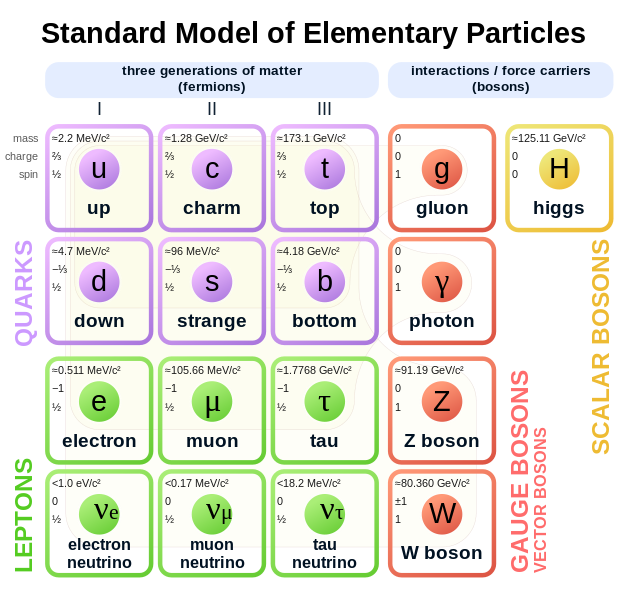
\includegraphics[width=\textwidth]{figures/intro/Standard_Model_of_Elementary_Particles.svg.png}
  \caption{
    The Standard Model of Particle Physics showing the twelve fermions and five bosons,
    their various properities (mass, charge, spin), labels (box and circle colors),
    and interactions (brown loops). Credit to Cush on wikipedia for
    providing this diagram freely accessible and usable for any purpose.
  }
  \label{fig:sm}
\end{figure}

The two lowest mass quarks -- the up and the down -- are the fundamental constituents of protons
and neutrons which make up the nuclei of atoms which make up all the day-to-day stuff we interact
with. These stay bound together within these nuclei via the strong nuclear force (mediated and
represented in \cref{fig:sm} by the gluon). These quarks and the top row of leptons also have an
electric charge enabling them to interact via with electromagnetic force (or equivalently exchange
photons). The electromagnetic force, represented and mediated by the photon, is the force
responsible for light and magnetism. The lowest mass charged lepton (electron) is also very
abundant -- most commonly residing in orbits around nuclei helping form atoms. Both experiments in
this thesis utilize beams of electrons that have been accelerated to high energies and then
impinge upon a material of high density to initiate interactions for further study.

The mathematical expressions to calculate how these particles interact are complicated. As
mentioned earlier, physicists are lazy and so we have developed a method to represent the specifics
of these interactions without needing to write down any of the long mathematical formulae. These
representations are called ``Feynman diagrams'' after the 20th century physicist Richard Feynman.
Feynman diagrams allow us to represent interactions by defining a set of ``vertices'' that are
allowed by our theory and then constructing processes from these vertices that include the in- and
out- going particles that we wish to study. The further calculation of these diagrams is a defined
process that has been written into various computer programs (I say this to emphasize that these
diagrams directly represent the mathematics that can be used to calculate them).
\cref{fig:brem-feynman} shows an example Feynman diagram representing the bremsstrahlung process
where a charged lepton (\(\ell^-\)) interacts with a nucleus (\(Z\)) via a photon (\(\gamma\)) and
then emits another photon before recoiling. We can see three verticies in this diagram: two
``fundamental'' vertices where the lepton and photon lines connect and one ``effective'' vertex
where the photon connects with the nucleus. The fundamental vertices are actually strictly defined
within the Standard Model, but the effective vertex represents a helpful approximation that is
accurate at the energy scales we are studying.\footnote{ The distinction between fundamental and
  effective vertices is not a well defined one. I find it helpful here, but it is not necessarily
  made elsewhere in physics literature. }

\begin{figure}
  \centering
  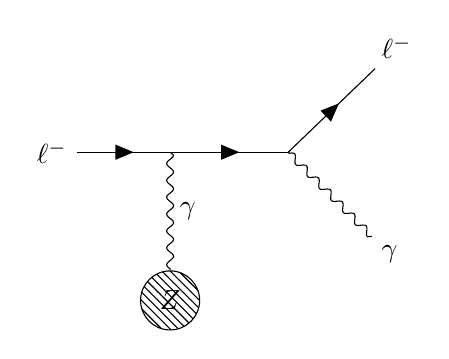
\begin{tikzpicture}
    \begin{feynman}
      \vertex (in) {\(\ell^-\)};
      \vertex [right=of in] (nuc);
      \vertex [below=of nuc, blob] (nucleus) {\(Z\)};
      \vertex [right=of nuc, dot] (emit);
      \vertex [above right=of emit] (recoil) {\(\ell^-\)};
      \vertex [below right=of emit] (decay) {\(\gamma\)};
      \diagram*{
      (in) -- [fermion] (nuc) -- [fermion] (emit) -- [fermion] (recoil),
      (nucleus) -- [photon, edge label'=\(\gamma\)] (nuc),
      (emit) -- [photon] (decay),
      };
    \end{feynman}
  \end{tikzpicture}
  \caption{
    Feynman diagram for the bremsstrahlung process.
  }
  \label{fig:brem-feynman}
\end{figure}

For the rest of this thesis, I intend to stay within this realm -- representing the theoretical
calculations being tested with these diagrams and limiting the scope of mathematical formulae
presented. Occasionally, the weight of these vertices which can be interpreted as the strength
of the interaction is presented along with the vertices in order to give a sense of scale.

%%%%%%%%%%%%%%%%%%%%%%%%%%%%%%%%%%%%%%%%%%%%%%%%%%%%%%%%%%%%%%%%%%%%%%%%%%%%%%%%

%%%%%%%%%%%%%%%%%%%%%%%%%%%%%%%%%%%%%%%%%%%%%%%%%%%%%%%%%%%%%%%%%%%%%%%%%%%%%%%%
%science.tex: Chapter on DM physics:
%%%%%%%%%%%%%%%%%%%%%%%%%%%%%%%%%%%%%%%%%%%%%%%%%%%%%%%%%%%%%%%%%%%%%%%%%%%%%%%%
\chapter{Dark Matter}
\label{chapter:dm}
%%%%%%%%%%%%%%%%%%%%%%%%%%%%%%%%%%%%%%%%%%%%%%%%%%%%%%%%%%%%%%%%%%%%%%%%%%%%%%%%

New phenomena have puzzled physicists throughout history, but the confusion surrounding dark matter
-- estimated to be roughly 85\% of the total matter in the universe -- is surely one of the biggest
puzzles. While many astronomical observations at various scales have confirmed the existence of
dark matter, we have not yet seen any observations of its particle interacting with our detectors.
This has ruled out many models for dark matter's particle nature, but there are still many more
available which can both explain the current observations of dark matter gravitational and
cosmological effects while skirting the limitations defined by the \emph{lack} of observation in
particle experiments.

\section{Dark Matter?}
The term \ac{dm} rose out of a brutally honest description of the present level of understanding.
``Matter'' originates from comparison to the particles that make ourselves up and with which we are
familiar -- both this new phenomena and our normal ``stuff'' interact gravitationally, attracting
other groups of ``matter'' into complex cosmological systems. The adjective ``dark'' refers to the
literal fact that we cannot see it with our telescopes. Other matter out in the universe can be
seen via the light that it gives off (or reflects), so the fact that this matter \emph{is not}
visible in this way motivates the adjective.

That is it. \acf{dm} is merely a shorthand for this aspect of the universe that is both known to
exist within the cosmos and whose particle nature is completely unknown.

\section{Evidence for Dark Matter}
\label{sec:dm:evidence}

The first (replicable) evidence physicists had for an unseen material floating throughout the
universe was the observation of galactic rotation curves
\cite{rubin-rotationcurve-1980,rotationcurve-2000}. These observations measure the speed of
different stars within a galaxy and compare this speed to the distance of that star from the center
of the galaxy. We can calculate this relationship using \ac{gr}
\cite{rotationcurve-predictions-2007} and the observations differ drastically from this
calculation. The stars within galaxies we've observed move much faster than \ac{gr} would predict
(\cref{fig:rotation-curve}) leaving us with two explanations: either \ac{gr} is not the correct
theory to use in this situation or there is more un-seen mass floating within the galaxy allowing
these stars to move faster without leaving the galactic orbit.

Other indirect measurements give us additional ways to access information about this odd phenomena.
Within the framework of \ac{gr}, since energy and mass actually warp the fabric of spacetime, we
expect to see light itself follow a bent path around massive objects - a phenomenum that is called
gravitational lensing and is observed and well modeled by \ac{gr}'s predictions
\cite{gravlensing-2004}. The accuracy of \ac{gr} within this context -- a mass and distance scale
similar to the rotation curve oddities also observed -- put more requirements on any modified
theory of gravity that could both explain the rotation curves and gravitational lensing.
Additionally, measurements on some of the largest scales and from the early universe display signs
of a certain mass density attributed matter that does not interact in the same ways as our normal
matter (called ``baryonic'' matter).

In the early universe, standard matter was compressed into high densities and existed at high
temperature creating a sea of plasma. Gravity attracts while pressure from the squeezing of this
plasma repulses which produces oscillations in the density of matter in space and time. The
repulsive pressure within the plasma originates from particles interacting electromagnetically with
each other, so the oscillations would be disrupted by the presence of extra matter interacting
gravitationally but not interacting electromagnetically. These \ac{bao} are imprinted on our
snapshot of this early-universe plasma, the \ac{cmb}, which we can measure with a high degree of
accuracy and fit to various models of what existed at this time of the universe. The best fit of
these models corresponds to only $\sim 5\%$ of the mass density being normal matter like we see
today (``baryonic'') while the rest is composed of material that only significantly interacts
gravitationally \cite{planck-cmb-2015}.

Additional astromomy observations from Type1a supernovae \cite{type1a-supernova-2010}, fitting
models of big bang nucleosynthesis \cite{nucleosynthesis-1998}, and constraints on non-particulate
theories explaining these phenomena (for example mini black holes
\cite{constraints-primordial-black-holes-2021}) all allow us to conclude pretty comfortably that
\ac{dm} exists as a particle in our universe.

\begin{figure}
  \centering
  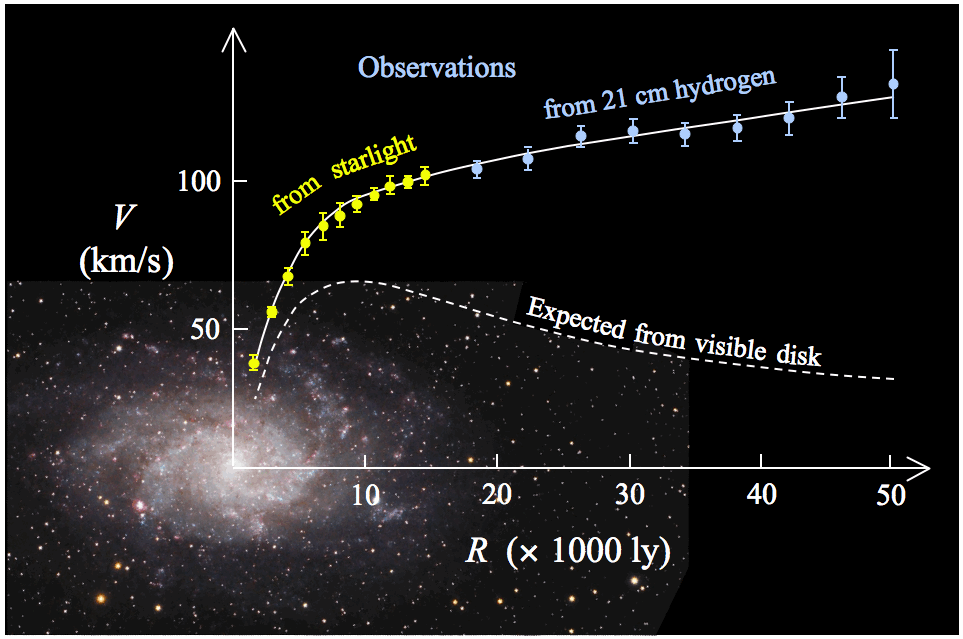
\includegraphics[width=0.6\textwidth]{figures/theory/rotation-curve-evidence-for-dm.png}
  \caption{
    Depiction of the velocity of stars within a galaxy as a function of their distance
    from the galactic center. The dotted line is a prediction of this relationship using
    \ac{gr} along with the mass tabulated from the visible starts while the data points
    (and the solid line fitted to them) are what are actually seen in galaxies today.
  }
  \label{fig:rotation-curve}
\end{figure}

\section{Particle Nature of Dark Matter}
The theoretical possibilities explaining \ac{dm} are broad \cite{darksectors-2016} even when
excluding ourselves to the assumption that the \ac{dm} phenomenum is explained by the existence of
a \ac{dm} particle. The \ac{cmb} observations are tied to very early on in the existence of the
universe, so it is natural to assume that this \ac{dm} particle has existed since the start of the
universe alongside our normal matter particles. With this in mind, we can outline a few criteria
that must be met by a proposed \ac{dm} candidate.
\begin{itemize}
  \item \textbf{Dark} There has been no detection of these particles via the light observed with our telescopes;
        therefore, the \ac{dm} has to not interact via the electromagnetic force.
  \item \textbf{Long Living} Measurements of \ac{dm}'s mass density and presence agree across time
        (from as early as the \ac{cmb} era), so \ac{dm} needs to have a long lifetime.
  \item \textbf{Universal Density} Since we can indirectly measure a \ac{dm} mass density on
        cosmological scales, we impose the requirement that any \ac{dm} model needs to allow for
        this density.
  \item \textbf{Thermal Relic} Both \ac{dm} and standard matter have similar
        cosmological densities, so we expect some interaction (even a weak one) should connect their
        origins to the early universe allowing both to exist from the Big Bang. This criterion is
        not as firm as the others (\ac{dm} models correctly describing the current observations while
        avoiding this criterion do exist); nevertheless, this criterion is well motivated and it is
        satisfied by all of the models for \ac{dm} studied in this work.
\end{itemize}
Even with these assumptions and the requirements they imply, there still exist a plethora of
theoretical models that can satisfy all of them.

The upside is that a thermal-relic assumption closely connects the mass of individual \ac{dm}
particles to the interaction strength it has with standard matter. In this assumption, the \ac{dm}
evolves along with the universe allowing its number density to follow the density of standard
matter until the standard matter does not have enough energy to produce more \ac{dm}. While the
universe continues to expand, the \ac{dm} continues to decay into standard matter until it becomes
too sparse to annihilate with itself and is thus ``frozen'' at a specific number density. Since
this ``frozen'' density changes depending on how easy it is for the \ac{dm} to interact with
standard matter, the ``frozen'' number density goes down as the interaction strength increases
(\cref{fig:number-density}). The additional requirement of the observed astronomical \emph{mass}
density connects the mass of individual \ac{dm} particles to their interaction strength with
standard matter.
\begin{equation}\label{eqn:dm-mass-interaction-strength-connection}
  m_\chi \leftrightarrow \text{observed mass density}
  \leftrightarrow \frac{dN}{dV} \leftrightarrow
  \text{thermal relic hypothesis} \leftrightarrow
  \langle\sigma v\rangle
\end{equation}
This connection allows us to define strict ``thermal relic targets'' which can help be measuring
sticks for how well our experiments search for \ac{dm} (these targets will appear in plots later).

\begin{figure}
  \centering
  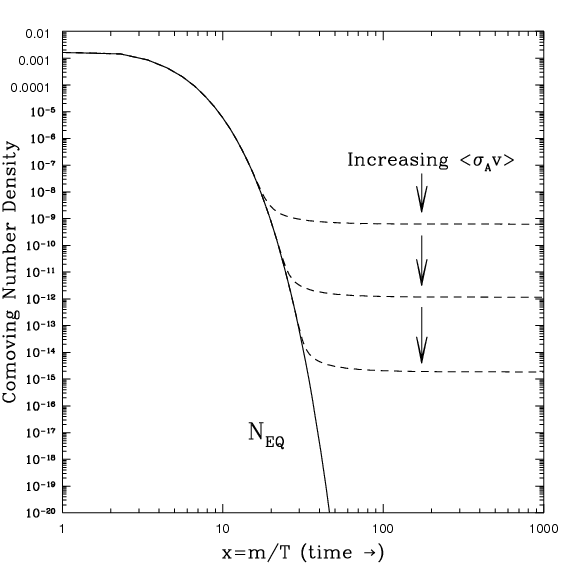
\includegraphics[width=0.5\textwidth]{figures/theory/number-density-at-freeze-out.png}
  \caption{
    From \cite{thermal-freezeout-diagram-1996}, the co-moving cosmological number density of \ac{dm} as a function of the universe
    temperature. As the universe cools, the number density decreases until the \ac{dm}
    becomes too sparse to interact with other \ac{dm} particles, ``freezing'' to a specific
    number density until today.
  }
  \label{fig:number-density}
\end{figure}

In addition to the connection between interaction strength and particle mass implied by the thermal
relic hypothesis, it also puts some loose bounds on mass of individual particles
(\cref{fig:dm-mass-scale}). If the mass is too low (approximately below the mass of the electron
$m_e$), then it is not feasible within our early-universe models to produce enough \ac{dm} to match
the observed \ac{dm} density currently frozen in. Similarly, if the mass is too high ($\gtrapprox
  100~\text{TeV}$), the \ac{dm} will be too strongly coupled to the standard matter and would be
over-produced.

\begin{figure}
  \centering
  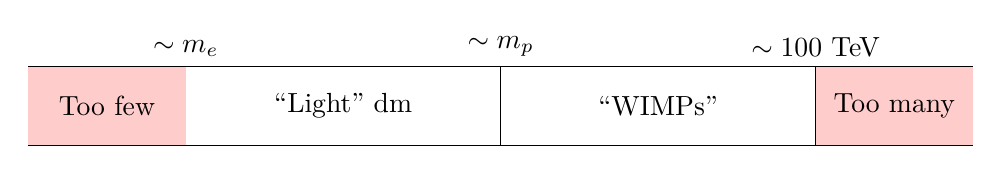
\begin{tikzpicture}
    % horizontal top/bottom lines
    \draw (0,0) -- (12,0);
    \draw (0,1) -- (12,1);
    % dividing lines along with relevant scale markers
    \draw (2,0) -- (2,1) node[above] {$\sim m_e$};
    \draw (6,0) -- (6,1) node[above] {$\sim m_p$};
    \draw (10,0) -- (10,1) node[above] {$\sim100~$TeV};
    % fill non-thermal ranges with light red
    \fill [red!20!white] (0,0) rectangle (2,1);
    \fill [red!20!white] (10,0) rectangle (12,1);
    % labels offering descriptions of ranges inside the boxes
    \node at (1,0.5) {Too few};
    \node at (4,0.5) {``Light'' \gls{dm}};
    \node at (8,0.5) {``WIMPs''};
    \node at (11,0.5) {Too many};
\end{tikzpicture}
  \caption{Mass scale of Thermal Relic \ac{dm}.
    The regions in red are excluded by applying the thermal relic assumption
    to our observations of the universe's early evolution.}
  \label{fig:dm-mass-scale}
\end{figure}

The mass scale of thermal relic \ac{dm} is further divided by the mass of the proton ($m_p$). Above
this threshold, the \ac{dm} could be interacting with standard matter through the standard Weak
Force (as described in \cref{chapter:intro}); thus, they are named \acp{wimp}. This phase space was
first searched due to its theoretical simplicitity: no new forces, just an extra particle (or two)
creating the clouds of \ac{dm} we see today. Unfortunately, these searches have not found evidence
of a \ac{wimp}-like signature\cite{supercdms-2018,damic-2020,xenon1t-2018} and the phase space has
become tighter and more exluded after many years of searching. Below $m_p$, the \ac{dm} requires a
new force which is even weaker than the Weak Force. In comparison to the heavier \acp{wimp}, this
category of \ac{dm} is called ``Light'' \ac{dm}.

\begin{figure}
  \centering
  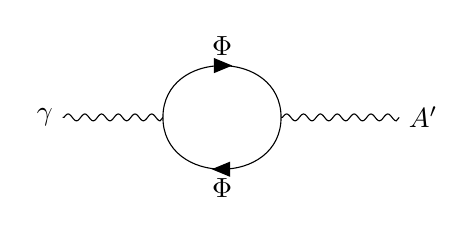
\begin{tikzpicture}
  \begin{feynman}
    \vertex (standard) {\(\gamma\)};
    \vertex [right=of standard] (loopleft);
    \vertex [right=of loopleft] (loopright);
    \vertex [right=of loopright] (dark) {\(A'\)};

    \diagram*{
    (standard)
    -- [photon] (loopleft)
    -- [fermion, half left, edge label=\(\Phi\)] (loopright)
    -- [photon] (dark),
    (loopright)
    -- [fermion, half left, edge label=\(\Phi\)] (loopleft),
    };
  \end{feynman}
\end{tikzpicture}

  \caption{Feynman diagram of how a massive field $\Phi$ could allow for a standard photon ($\gamma$)
    to mix with a dark photon ($A'$).}
  \label{fig:photon-mixing}
\end{figure}

In general, the definition of a new force of nature is not well constrained; however, we can define
a ``baseline'' model that can represent more concrete theories in the context of our experiments.
For this situation, we postulate the existence of a massive gauge boson that represents an
additional $U_D(1)$ symmetry of nature. Since this additional symmetry has the same structure as
the electromagnetic interaction whose gauge boson is the standard photon, we generally refer to
this postulated massive boson as a dark photon. Without any additional assumptions, this new dark
photon does not interact with any standard matter, so we also assume that some previously-unknown
massive fields are able to interact with both. These other fields need to be sufficiently massive
(or sufficiently weakly coupled) so that they only allow the standard and dark photons to weakly
mix. \cref{fig:photon-mixing} diagrams how the standard and dark photons mix which can then be
effectively represented by a new vertex in our model.
\begin{equation}\label{eqn:dark-photon-ll-vertex}
  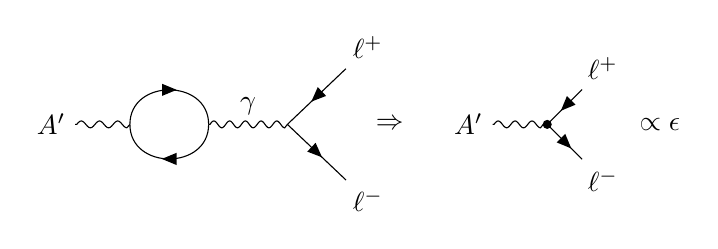
\begin{tikzpicture}
    \begin{feynman}[inline]
      \vertex (dark1) {\(A'\)};
      \vertex [right=of dark1] (loopleft);
      \vertex [right=of loopleft] (loopright);
      \vertex [right=of loopright] (gamma);
      \vertex [above right=of gamma] (ellplus1) {\(\ell^+\)};
      \vertex [below right=of gamma] (ellminus1) {\(\ell^-\)};

      \vertex [right=of gamma] (arr) {\(\Rightarrow\)};

      \vertex [right=of arr] (dark2) {\(A'\)};
      \vertex [right=of dark2, dot] (vtx) {};
      \vertex [above right=of vtx] (ellplus2) {\(\ell^+\)};
      \vertex [below right=of vtx] (ellminus2) {\(\ell^-\)};

      \diagram*{
      (dark1)
      -- [photon] (loopleft)
      -- [fermion, half left] (loopright)
      -- [photon, edge label=\(\gamma\)] (gamma),
      (loopright) -- [fermion, half left] (loopleft),
      (ellplus1) -- [fermion] (gamma) -- [fermion] (ellminus1),
      };

      \diagram*{
      (dark2) -- [photon] (vtx),
      (ellplus2) -- [fermion] (vtx) -- [fermion] (ellminus2),
      };
    \end{feynman}

    \node [right=of vtx] (eqn) {\(\propto \epsilon\)};
  \end{tikzpicture}
\end{equation}
where the mixing strength $\epsilon$ encapsulates the effect of a massive field $\Phi$ at the energies
of our experiments (presumably low enough to avoid creation of a $\Phi$ directly) and is generally
small ($\ll 1$).

This new vertex within our model for the universe enables a new process to occur: so-called ``Dark
Bremsstrahlung'' (dark brem) where a charged particle exchanges a standard photon with a nucleus
and then emits a dark photon and recoils.

\begin{figure}
  \centering
  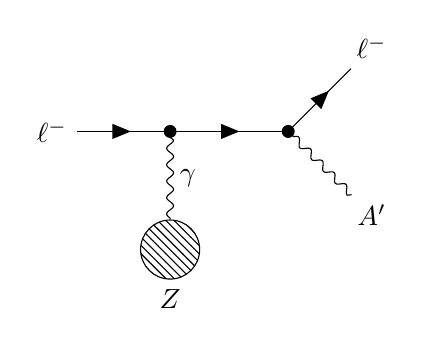
\begin{tikzpicture}
  \begin{feynman}
    \vertex (in) {\(\ell^-\)};
    \vertex [right=of in, dot] (nuc) {};
    \vertex [below=of nuc, blob, label={below:\(Z\)}] (nucleus) {};
    \vertex [right=of nuc, dot] (emit) {};
    \vertex [above right=of emit] (recoil) {\(\ell^-\)};
    \vertex [below right=of emit] (decay) {\(A'\)};
    % \vertex [above right=of decay] (chi2) {\(\overline{\chi}\)};
    % \vertex [below right=of decay] (chi1) {\(\chi\)};

    \diagram*{
    (in) -- [fermion] (nuc) -- [fermion] (emit) -- [fermion] (recoil),
    (nucleus) -- [photon, edge label'=\(\gamma\)] (nuc),
    (emit) -- [photon] (decay),
    % (emit) -- [photon, edge label'=\(A'\)] (decay),
    % (chi2) -- [fermion] (decay) -- [fermion] (chi1),
    };
  \end{feynman}
\end{tikzpicture}

  \caption{
    Feynman diagram for the dark brem process.
  }
  \label{fig:dark-brem-feynman}
\end{figure}

But what happens to the dark photon after it interacts with standard matter via this vertex? It
cannot be the long-lived \ac{dm} we view in the universe today because this vertex allows for it to
decay \emph{back} into standard matter eventually (and in some models, rather quickly). This is
where we expand on the idea of a ``dark sector''. In this description of \ac{dm}, we already have a
dark photon representing some force and a very heavy field that can interact with it. Suppose this
``dark sector'' also has other particles (like the standard sector) -- one (or more) of which could
be long-lived and represent the \ac{dm} we observe in the universe today (so-called ``\ac{dm}
candidates''). We can further partition this category of models depending on what happens to the
dark photon after we produce it within an experiment.

\section{Invisible Signature}
\label{sec:dm:invisible}

One of the simplest options is to hypothesize another particle that can take on the role of
long-lived \ac{dm} and only interact ``within'' this dark sector (i.e. it only interacts with the
dark photon from our point of view). Calling this particle $\chi$ (and its anti-particle
$\overline{\chi}$), we then have an additional dark sector vertex.
\begin{equation}
  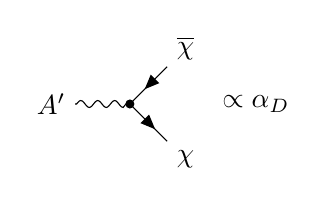
\begin{tikzpicture}
    \begin{feynman}[inline]
      \vertex (dark) {\(A'\)};
      \vertex [right=of dark, dot] (vtx) {};
      \vertex [above right=of vtx] (ellplus) {\(\overline{\chi}\)};
      \vertex [below right=of vtx] (ellminus) {\(\chi\)};

      \diagram*{
      (dark) -- [photon] (vtx),
      (ellplus) -- [fermion] (vtx) -- [fermion] (ellminus),
      };
    \end{feynman}

    \node [right=of vtx] (eqn) {\(\propto \alpha_{D}\)};
  \end{tikzpicture}
\end{equation}
where $\alpha_D$ is a parameter representing the strength of this dark sector interaction, limited
to be below $1$ but usually much larger than $\epsilon$ so that this interaction is more likely
than the one with standard matter.
If the mass of the dark photon is greater than twice the mass of the $\chi$ ($m_{A'} > 2m_\chi$),
then this vertex can occur immediately after a dark photon is produced within an experiment.
Since the $\chi$ does not interact with our normal \ac{sm} particles, the energy
they have is ``lost'' from our perspective. \cref{part:ldmx} focuses on a proposed experiment
designed to precisely measure all of the \emph{visible} energy so that this ``invisible signature''
of DM being produced could be observed.

When comparing analyses across \ac{dm} search literature,
it is common to parameterize the \ac{dm} phase space with an
effective interaction strength $y$ and the mass of the candidate \ac{dm}
$m_\chi$ that would constitute the astronomical \ac{dm} observed today.
The parameter $y$ is related to the parameters of our ``baseline'' model by
$$
  y = \alpha_D \epsilon^2 \left(\frac{m_\chi}{m_{A'}}\right)^4
$$
where we make standard, benchmark choices $\alpha_D = 0.5$ and $m_{A'} = 3m_\chi$
when converting from $(\epsilon,m_{A'})$ to $(y,m_\chi)$.

\section{Visible Signature}
\label{sec:theory:visible}

There is no a priori reason for $m_{A'} > 2 m_\chi$ -- the quantum nature of these fundamental
particles allows for ``virtual'' dark photons to have more or less energy than precisely $m_{A'}$
allowing them to mediate the interactions between $\chi$ and \ac{sm} particles, so we must
accomodate the possiblity that $m_{A'} < 2 m_\chi$. In this case, there would be a significant
probability that the dark photon, after it is produced, would convert \emph{back} into \ac{sm}
particles. Since these decay products are observable by our detectors, this signature is called
visible.

These visible signatures are a bit more complex to model due to the fact that both a production
process and a decay process need to occur according to the model of \ac{dm} we are testing. With
this in mind, many models that provide more detail about how particles exist within a dark sector
have been created, each of which providing a specific estimate for production and decay rates.
\cref{part:hps} focuses on an experiment looking for these visible signatures and my work
specifically was investigating one of these more intricate dark sector models in detail.
\cref{sec:hps:simps} provides more detail on the dark sector model studied in this work.


\part{LDMX} \label{part:ldmx}
%%%%%%%%%%%%%%%%%%%%%%%%%%%%%%%%%%%%%%%%%%%%%%%%%%%%%%%%%%%%%%%%%%%%%%%%%%%%%%%%
% experiment.tex: Chapter describing the experiment
%%%%%%%%%%%%%%%%%%%%%%%%%%%%%%%%%%%%%%%%%%%%%%%%%%%%%%%%%%%%%%%%%%%%%%%%%%%%%%%%
\chapter{Light Dark Matter eXperiment}
\label{chapter:ldmx:experiment}

\ac{ldmx} is a proposed fixed-target experiment aiming to definitively explore
the thermal relic light dark matter phase space. Even as a proposed experiment, it has a detailed
plan for construction, a beam already in construction, and well established connections
with current technologies used within \ac{hep}. While \ac{ldmx} is not yet built,
it has a well formulated simulation infrastructure that can realistically model
how the detector design responds to various types of interactions happening within it.

\section{Missing Momentum Signature}
\ac{ldmx} aims to search for an invisible signature -- with known incident particle kinematics,
measuring the outgoing particle kinematics allows for a natural comparison. All of the incoming
momentum must exit somehow and so if the detector is unable to observe some momentum (some momentum
is ``missing'') frequently enough, we can conclude that some other, previously-unknown, process
is taking place and carrying momentum away from the experiment.

Precisely understanding both the incident and outgoing momenta requires knowledge of the currently
known processes and how to detect the particles they produce. The center of \cref{fig:ldmx-bkgd-staircase}
displays an ordering of known processes based on how frequently they occur given an incident electron 
with \qty{4}{\giga\electronvolt} of energy. This chart can be broken into three regions.

The blue region at the top are the most frequent types of processes,
but are simultaneously less complicated. The processes in this region (as the right side shows)
puts requirements on the design of the \ac{ecal}, making sure it can quickly and faithfully
reconstruct the outgoing energy.  The \ac{ecal} must be able to veto the first several
orders of magnitude in basic energy fluctuations including simple interactions in the
target like bremsstrahlung or trident production of an electron-positron pair.

Entering the pink region is where the background processes
become rarer and more complicated. One of the first ways to partition these backgrounds is
whether charged secondary particles are produced within the target. These ``prompt'' backgrounds
help define the recoil tracker's design and are thus left to be caught by it. More frequently,
a photon is produced within the target (which is not observable by the tracker) and then undergoes
complicated photon-nuclear interactions within the \ac{ecal} producing particles that are difficult
for the \ac{ecal} itself to observe. The \ac{hcal} is able to detect the presence of these hadrons
and muons, acting as a ``pure'' veto in the sense that the signal process should not create
significant activity within it.

All of these subsystems can collaborate to help \ac{ldmx} reject known \ac{sm} backgrounds
down to $\sim 10^{-16}$ fraction of all incoming electrons where extremely rare known processes
that produce invisible products (neutrinos $\nu$) begin to emerge.

Detailed study of the missing momentum search strategy\cite{ldmx-whitepaper,ldmx-photon-reject-2020,ldmx-8gev-2023} shows that \ac{ldmx} can reject all simulated backgrounds to a relative rate of $\sim 10^{-14}$.
This performance is accomplished through the basic design drivers outlined above and in \cref{fig:ldmx-bkgd-staircase}, but also through the additional granularity of the \ac{ecal} enabling
the use of a \ac{bdt} to distinguish between background and signal events using features of the
showers within the \ac{ecal}.

\begin{figure}
	\centering
	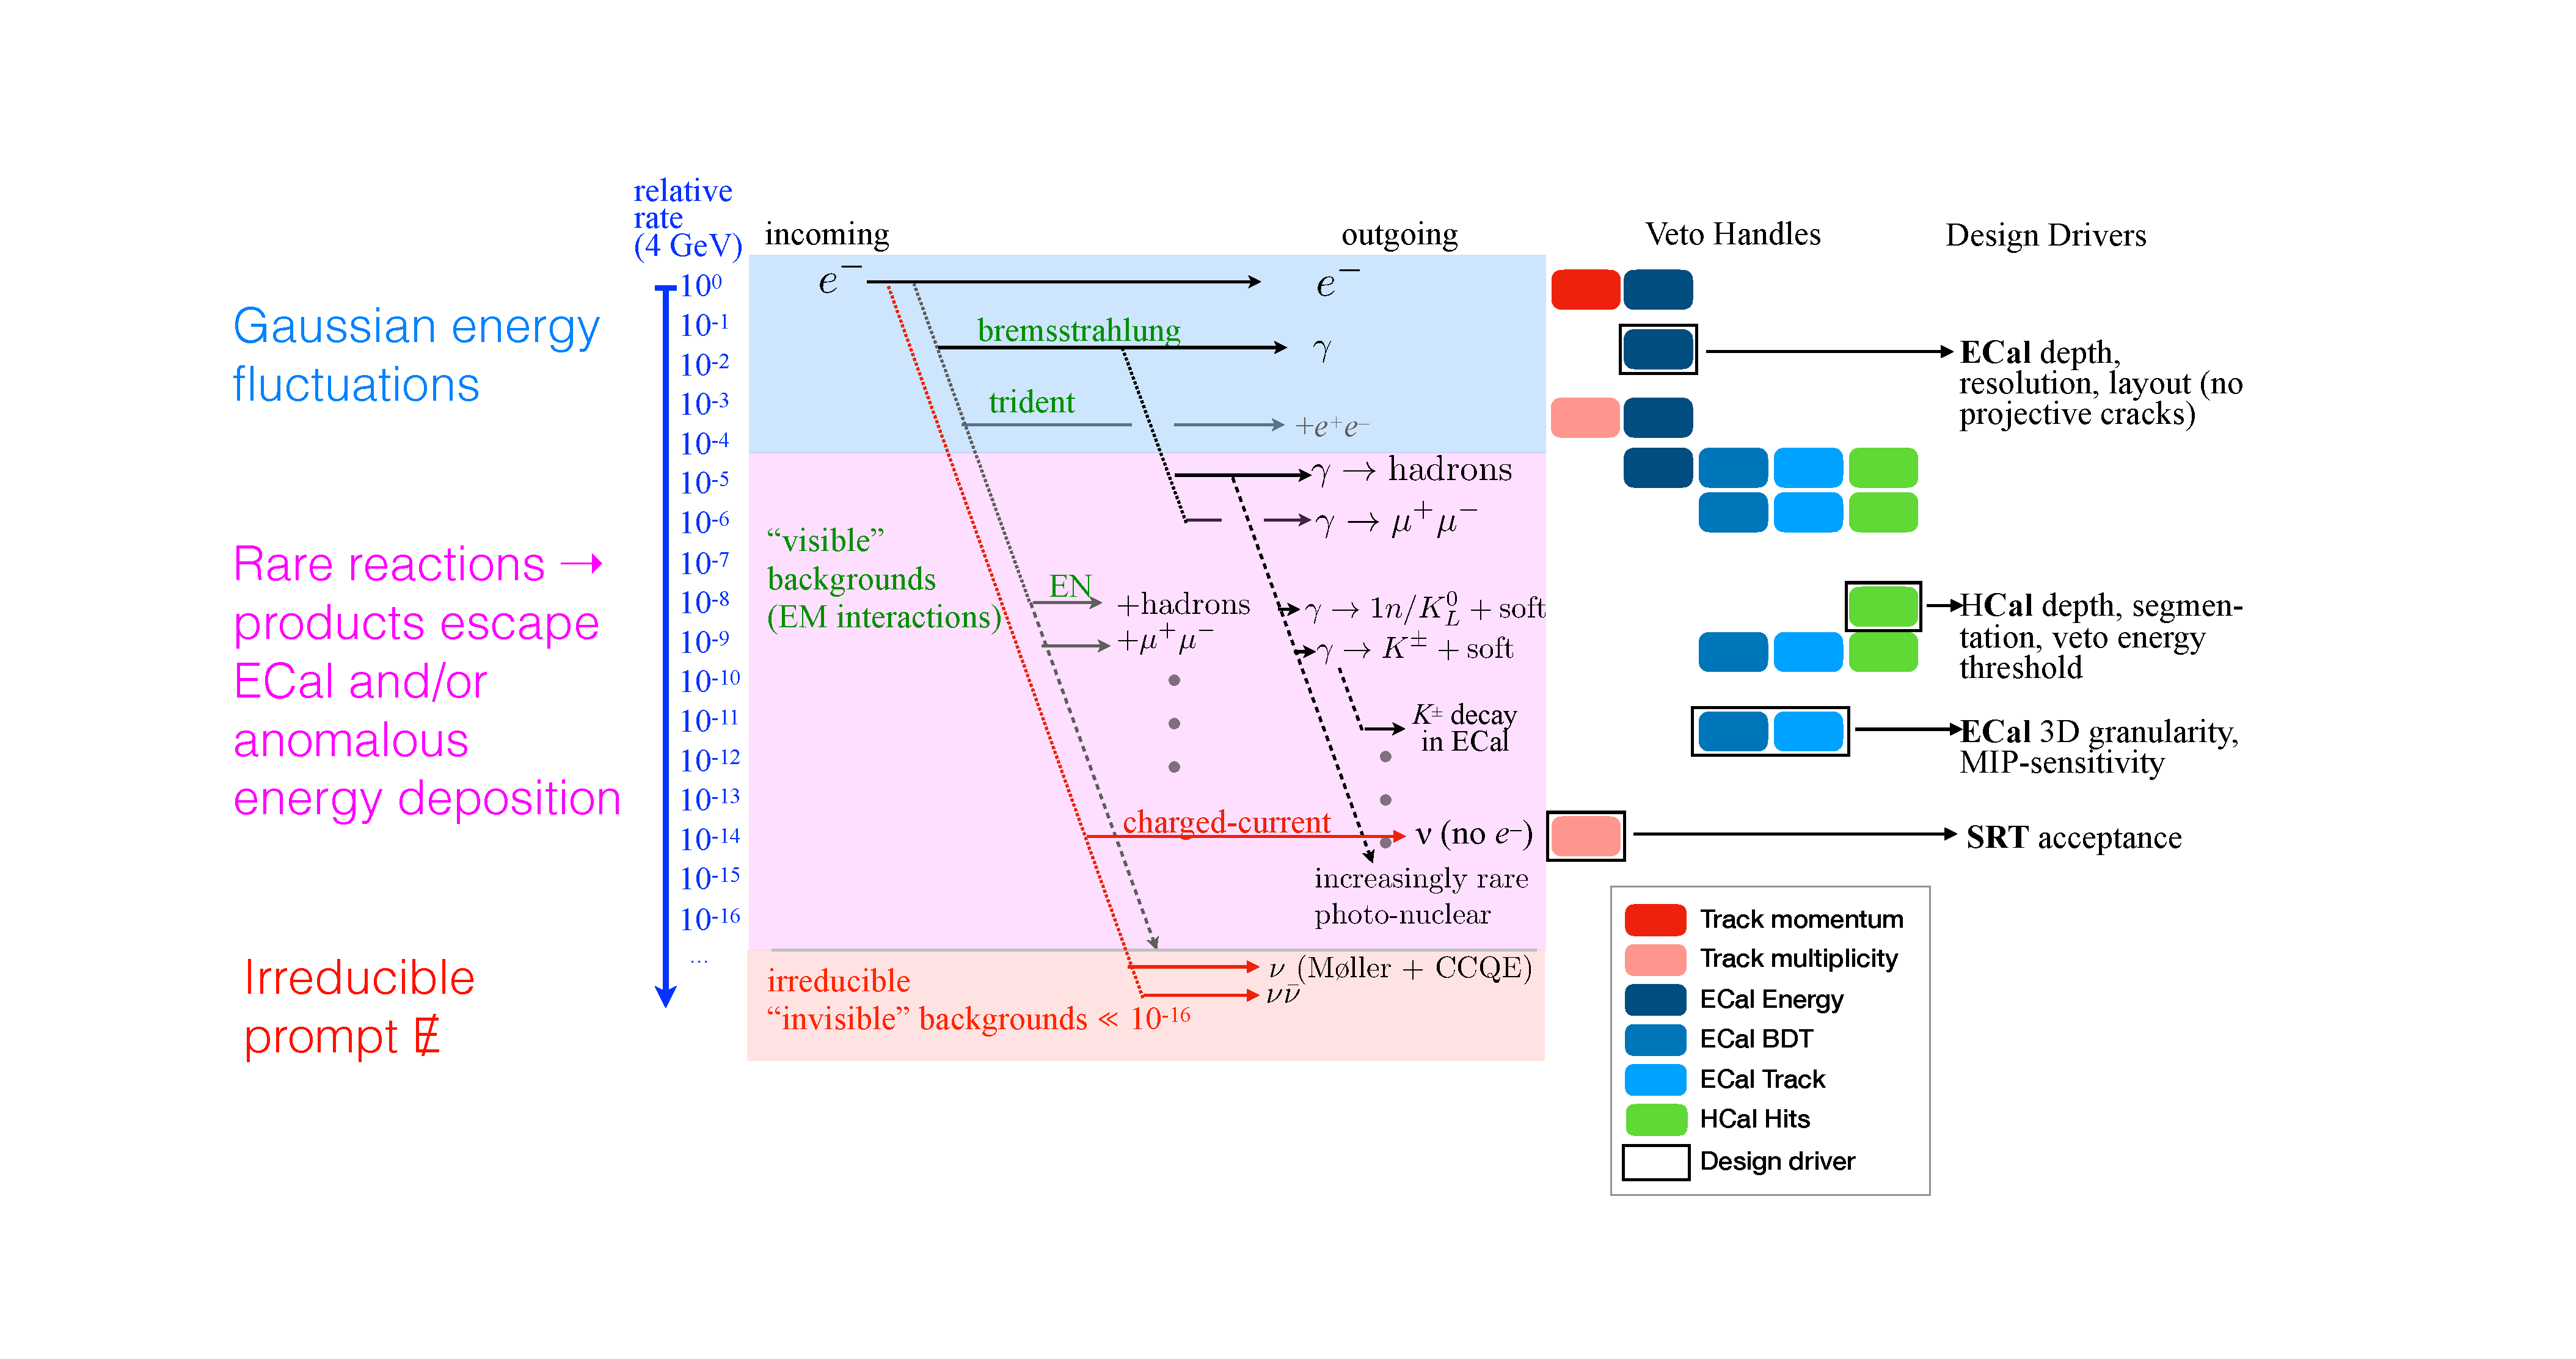
\includegraphics[width=\textwidth]{figures/ldmx/experiment/reaction_staircase_with_designDrivers.pdf}
	\caption{
		Diagram showing relative rates of background processes within LDMX along with
		how they motivate various aspects of the design. $\slash{E}$ stands for ``missing''
		energy or energy that is ``lost'' to neutrinos that are extremely unlikely to be
		detectable within LDMX.
	}
	\label{fig:ldmx-bkgd-staircase}
\end{figure}

\todo[diagrams]{
	Include diagrams of the primary backgrounds to help give context.
}

Cycles of detailed simulation and redesign has led to a detailed construction plan for the \ac{ldmx}
detector apparatus. The subsequent sections of this chapter detail this design as well as
the beam it is expected to receive.

\section{The Beam Line}
\todo[correctness]{Confirm correctness of LDMX beamline quick facts.}
\ac{ldmx} is planned to be situated at the end of the Linear Accelerator (Linac) at SLAC National Accelerator
Laboratory. The SLAC Linac can provide high energy, high rate, and low intensity electron beams for
the various experiments it hosts. Specifically, the Linac Coherent Light Source (LCLS) is
used to guide the beam (of a certain energy) towards the experimental hall - the upgraded
phase of LCLS (LCLS II \cite{lcls-ii}) is currently under construction and is what will
be used for running with \ac{ldmx}.

The experiment is hosted in End Station A (ESA) at SLAC which requires an additional upgrade to the
accelerator complex in order to recieve its beam. LESA (Linac to ESA) \cite{lesa-design} is also currently being
constructed and will be ready for test beam in early 2025. Part of the infrastructure that
transfers the beam to ESA (Sector 30 Transfer Line -- S30XL) is already constructed and LDMX
components are expected to participate in a test beam run in summer 2024.

\section{Detector Design}
As described above, \ac{ldmx} is a missing momentum experiment 
and its design is focused on measuring \emph{both} the
incoming and outgoing momenta of charged particles interacting with a thin target such that
any momentum given to undetectable (dark) particles can be precisely determined.
In addition, the energy of neutral particles must be measured.
This design has led to four subsystems each with specialized roles.\footnote{
	These subsystems also take on additional roles when the full breadth of the
	\ac{ldmx} physics program is taken into account.
	This description just focuses on the \ac{dm} search.
}
\begin{enumerate}
	\item \textbf{Tracker} Measure charged particle momenta both before (``Tagger'') and after (``Recoil'') the target.
	\item \textbf{Electromagnetic Calorimeter} (\ac{ecal}) Measure the total energy of electrons, positrons, and photons.
	\item \textbf{Hadronic Calorimeter} (\acs{hcal}) Veto additional particles difficult for other subsystems to measured (muons, pions, hadrons,...).
	\item \textbf{Trigger Scintillator} Count the number of electrons incident on the target in time to make a trigger decision (more on what a ``trigger'' is below).
\end{enumerate}
\cref{fig:ldmx-det} displays these subsystems in a diagram along with a representation of
a dark brem interaction occurrring within the target. \cref{fig:ldmx-render} shows a rendering
of the detector design.

The Tracker (purple in \cref{fig:ldmx-det}) is a thin silicon strip detector modeled after the
\ac{hps} tracker. These silicon strips are arranged in layer pairs where one layer is angled
slightly askew relative to the other in the pair to enable reconstruction of three dimensional hit
locations. The part of the tracker upstream of the target (to the left in \cref{fig:ldmx-det}) is
named the ``tagger'' since its purpose is to measure the incident electrons' momenta, rejecting
electrons' with momentum below \qty{30}{\percent} of the expected beam momentum. The tagger is situated within
the bulk of the magnetic field enabling highly precise measurement of this incident momentum. The
other part of the tracker located downstream of the target (to the right in \cref{fig:ldmx-det}) is
named the ``recoil'' tracker since its job is to measure the momenta of all charged particles
recoiling from interactions within the target. While it is not located within the magnet volume, it
is still situated within the fringe field, allowing functional momentum resolution.

In many \ac{hep} experiments, a ``trigger'' system is necessary in order to filter data defined to
be interesting by the experiment from the wealth of uninteresting (or normal) data that is expected
to be collected at a much higher rate. These trigger systems are the first filter that any data goes
through and are designed to help the experiment obtain a statistically large data sample without
collecting an overwhelming amount of data. The \ac{ecal} is the primary detector subsystem responsible
for making this trigger decision due to its excellent energy resolution and fast measurement capabilities.
As a search for \emph{missing} momentum, the \ac{ecal} requires less than \qty{30}{\percent} of the incoming
beam energy to be observed within the first twenty sensitive silicon layers.

The Trigger Scintillator (yellow-orange in \cref{fig:ldmx-det}) is designed to help inform the trigger
decision by counting the number of electrons present within the detector. It is made of layers of vertically
segmented bars of plastic scintillator. These layers are arranged in pairs where the layers within
each pair are offset from one another to cover any gaps between the bars. These bars are readout in
time to be used within a trigger decision combined with information from the \ac{ecal} and \ac{hcal}.

The \ac{hcal} (green in \cref{fig:ldmx-det}) is a sampling calorimeter made up of alternating
layers of steel absorber and plastic scintillator bars. The \ac{hcal} is further subdivided into
the ``side'' \ac{hcal} which is situated around the \ac{ecal} and the ``back'' \ac{hcal}
downstream of the \ac{ecal}. The back \ac{hcal} has the orientation of the scintillator bars
alternate between vertical and horizontal so that clusters and tracks can have three-dimensional
coordinates more preceisely identified.

The \ac{ecal} (blue in \cref{fig:ldmx-det}), as a primary volume of interest within the analysis
discussed here, is given its own diagram \cref{fig:ldmx-ecal}. The \ac{ecal} is also a sampling
calorimeter; however, it uses a different absorber material and a different sensing mechanism to
more precisely measure the energy of electrons, positrons, and photons. The calorimeter is constructed
out of seventeen layers each consisting of tungsten absorber, service materials, and sensitive silicon
sensors. Each of the layers of the detector has two sub-layers of sensitive silicon sensors and each
of these sub-layers are built up out of the hexagonal High-Density boards designed for the CMS
Phase II High Granularity Calorimeter upgrade\cite{cms-phase-2-tdr}. These hexagons are arranged in a ``flower''
providing excellent transverse resolution of shower location and shower shape. The layers are built
and arranged in order to space the sensitive silicon sub-layers to give good longitudinal resolution
of showers as well. In total, the designed \ac{ecal} has more than one hundred thousand channels that
can each individually detect particles depositing energies from $\approx \qty{0.1}{\mega\electronvolt}$ up to
$\approx\qty{1}{\giga\electronvolt}$\todo[confirm]{Confirm extimate of maximum single-hit energy}.
This high granularity calorimeter gives \ac{ldmx} excellent discrimination power
since it can measure the amplitude and location of several incident particles\todo[evidence]{provide
	evidence for this precision claim}.
Due to its high performance, the \ac{ecal} is a primary tool for
both designing a trigger decision (with the aid of the Trigger Scintillator's electron count) as well
as downstream analysis separating \ac{sm} background processes from potential \ac{dm} signal.

\begin{figure}
	\centering
	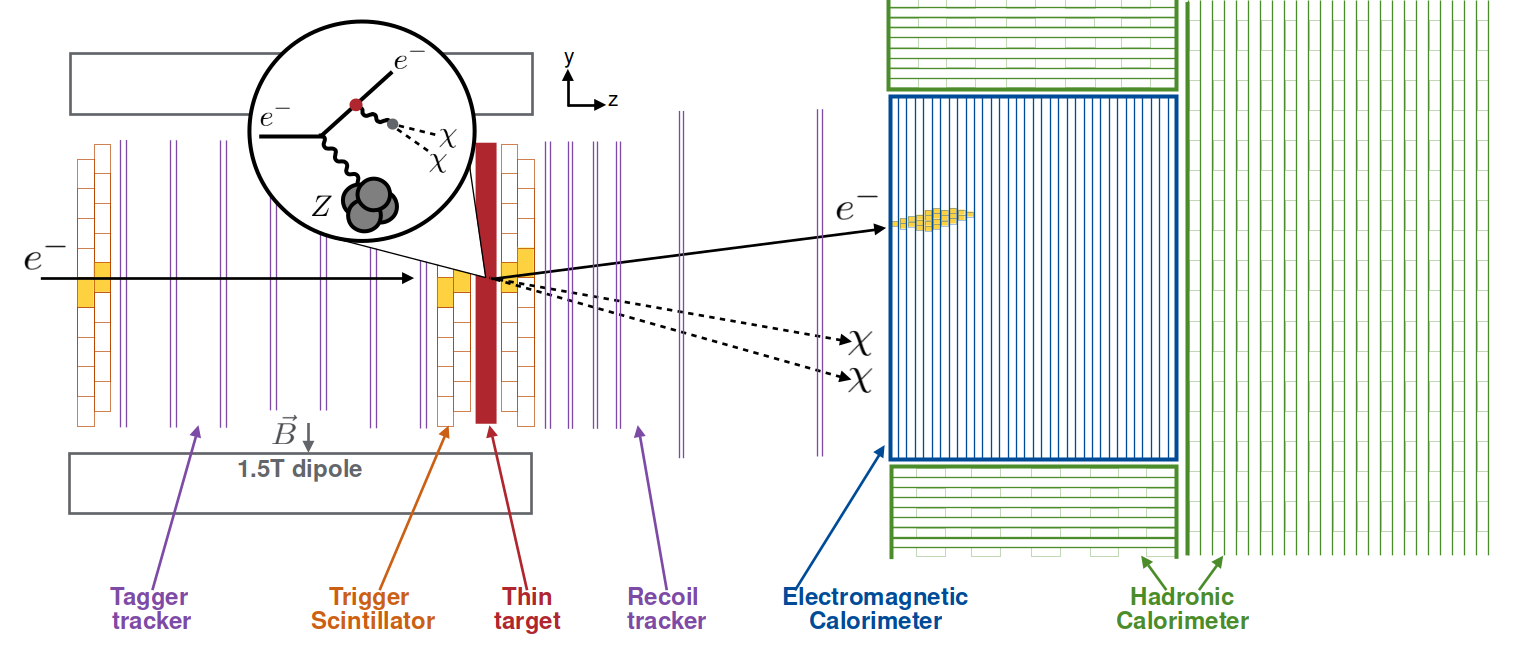
\includegraphics[width=0.9\textwidth]{figures/ldmx/experiment/detector.png}
	\caption{
		Diagram of LDMX detector apparatus with a representation of a signal event where
		a dark brem occurs within the target. Diagram is not to scale. Credit to Christian Herwig
		for original development of diagram.
	}
	\label{fig:ldmx-det}
\end{figure}

\begin{figure}
	\centering
	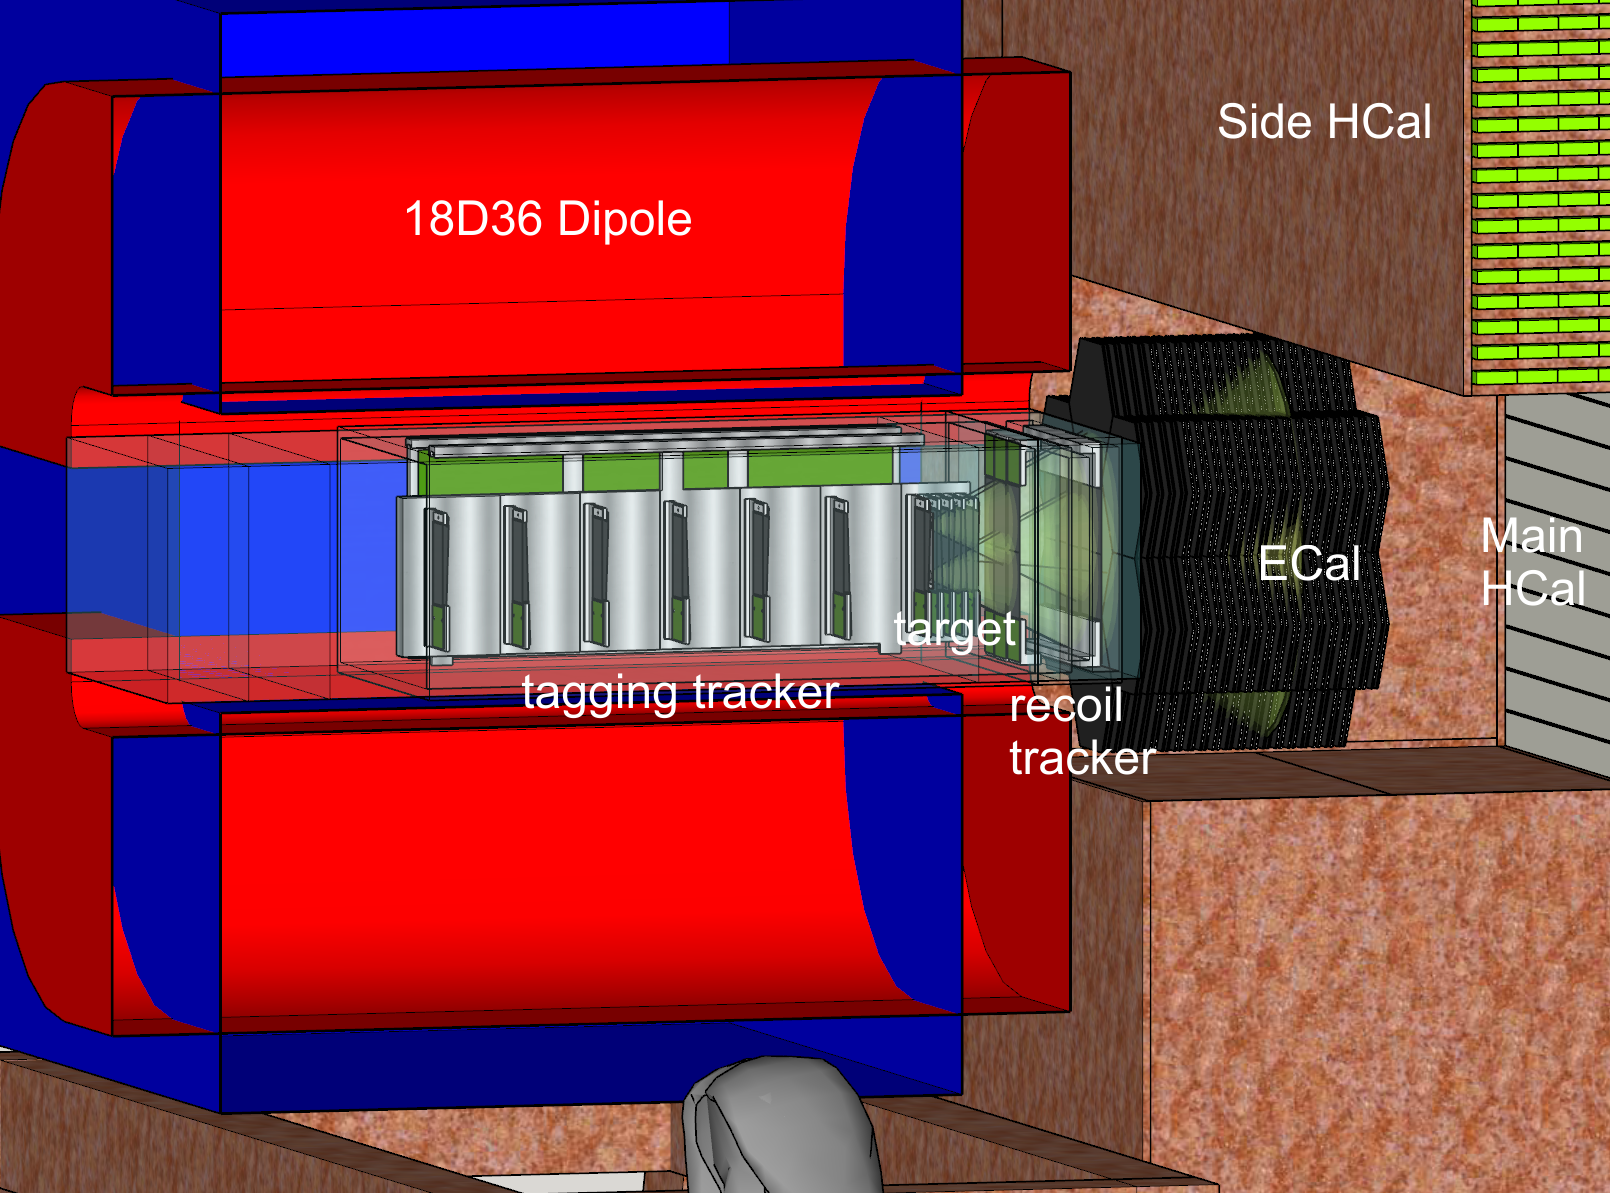
\includegraphics[width=0.9\textwidth]{figures/ldmx/experiment/LDMX_FOA_CLOSE.PNG}
	\caption{
		Rendering of LDMX detector apparatus focusing on tracker, target, and ECal.
		The magnet would fully encompass the tracker, target and trigger scintillator.
	}
	\label{fig:ldmx-render}
\end{figure}

\begin{figure}
	\centering
	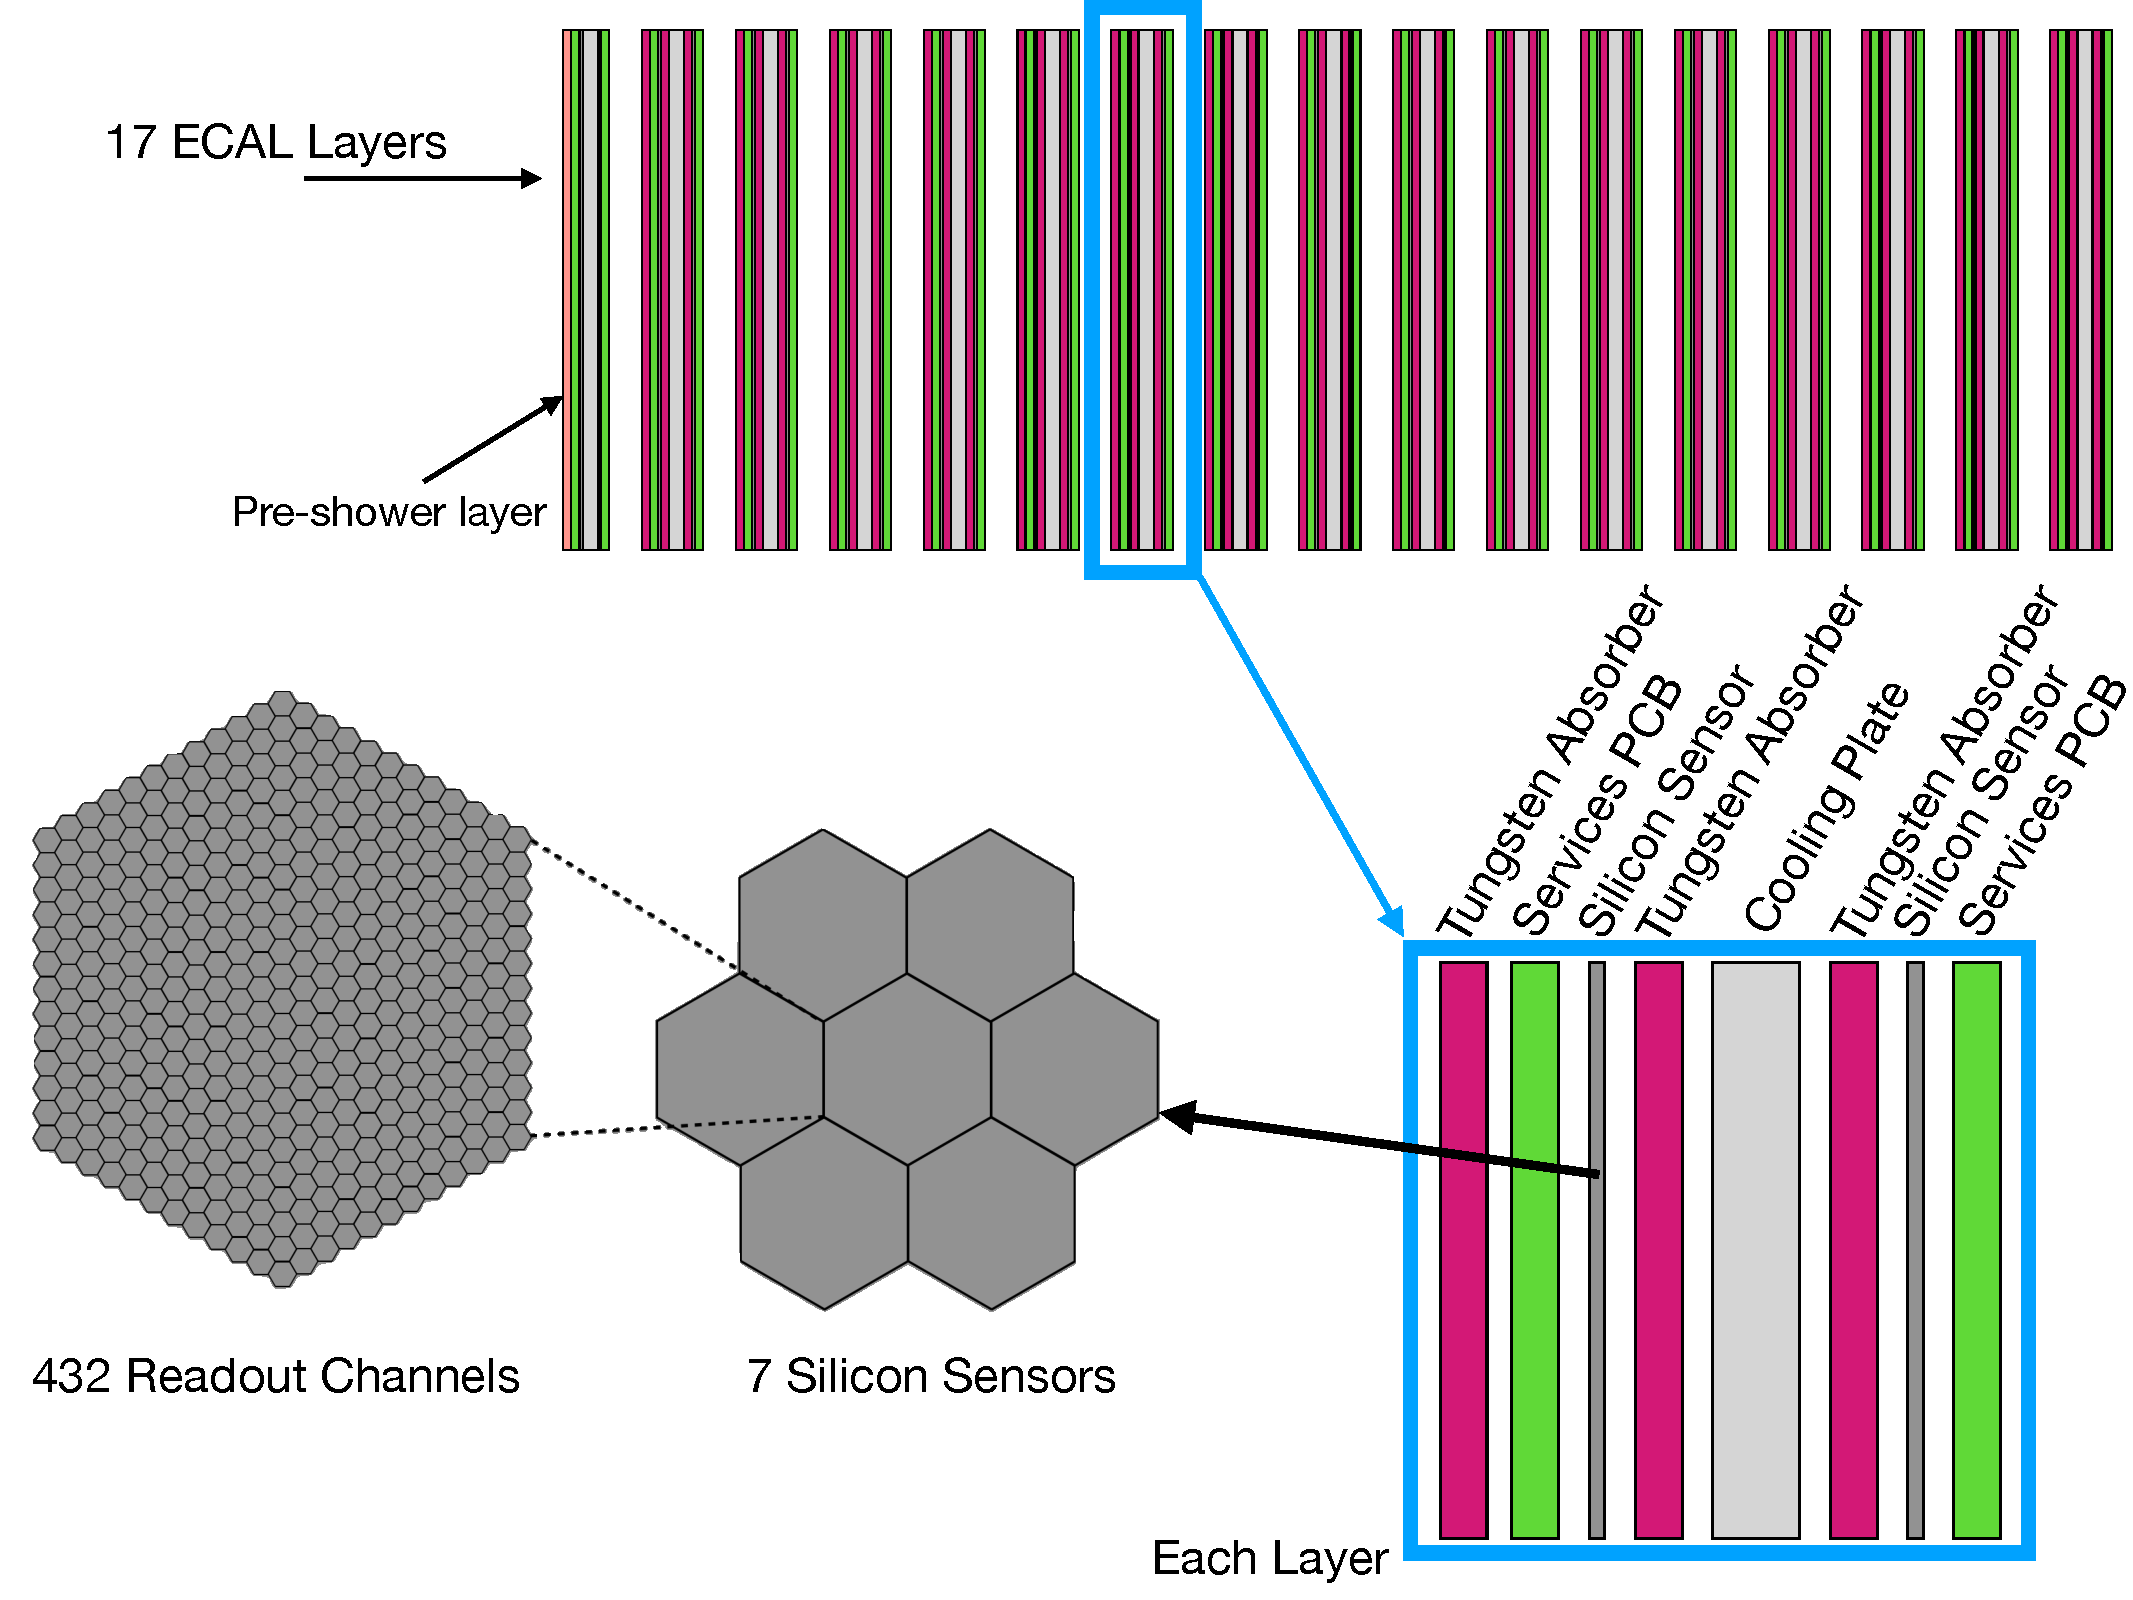
\includegraphics[width=0.9\textwidth]{figures/ldmx/experiment/ecal.pdf}
	\caption{
		Diagram of LDMX \ac{ecal} construction showing the longitudinal segmentation
		(top and bottom right) and the transverse segmentation (bottom left).
		Credit to Joe Muse.
	}
	\label{fig:ldmx-ecal}
\end{figure}

%%%%%%%%%%%%%%%%%%%%%%%%%%%%%%%%%%%%%%%%%%%%%%%%%%%%%%%%%%%%%%%%%%%%%%%%%%%%%%%%
% simulation.tex: Chapter on MC production:
%%%%%%%%%%%%%%%%%%%%%%%%%%%%%%%%%%%%%%%%%%%%%%%%%%%%%%%%%%%%%%%%%%%%%%%%%%%%%%%%
\chapter{Simulation}
\label{chapter:ldmx:simulation}
%%%%%%%%%%%%%%%%%%%%%%%%%%%%%%%%%%%%%%%%%%%%%%%%%%%%%%%%%%%%%%%%%%%%%%%%%%%%%%%%

\ac{ldmx} (like many other HEP experiments) uses an intricate software stack in order to realistically and efficiently simulate particle interactions with the detector, emulate the electronics that would be used to measure these interactions, and reconstruct the output of these electronics into physically-understandable variables.
These software tasks are accomplished by a wide swath of different software packages, some of which custom-written for \ac{ldmx}, most of which written in C++.
This chapter is focused on describing this simulation infrastructure -- focusing particularly on parts of the infrastructure I was involved in -- while also pointing out areas that are expected to remain constant in the presence of data gathered from a real detector.
After a discussion of general data processing, I move into discussing the specific samples
used to do this simulation study.

\section{General Data Process}
One of the core principles helping organize HEP data is the concept of an ``event.'' In the context
of \ac{ldmx}, an event is the data collected within a small window of time around the arrival of a
beam electron into our detector apparatus. In essence, each event within the software is
independent from one another however they all share a similar structure to the information they
hold. A natural example is a data table: a row has the same values in each of its columns as all
the other rows. Events behave the same way; however, unlike a data table, the structure of an event
can be more intricate than simply a series of values corresponding to different column titles.
While our basic ``unit'' of data is an event, we require many events in order to make statistical
conclusions about our data; thus, we have developed an ``event processing framework'' that allows
us to unify the various aspects of processing the data held within an event.

\begin{figure}
  \centering
  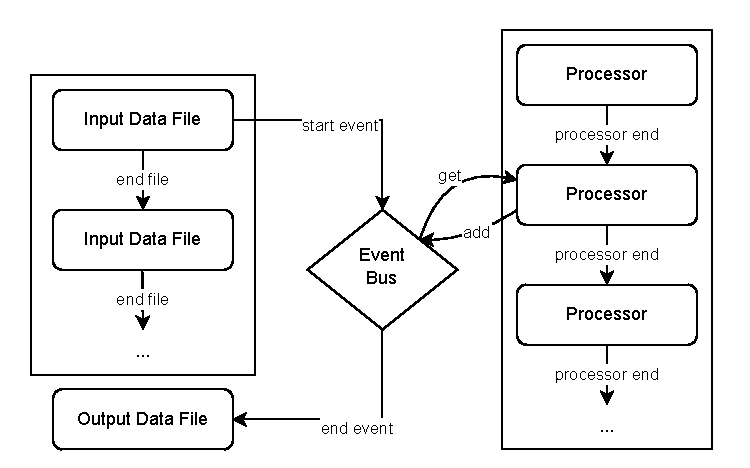
\includegraphics[width=0.9\textwidth]{figures/ldmx/simulation/FrameworkFlowChart.drawio.pdf}
  \caption{Flow chart of how data is processed in the \ac{ldmx} framework. Each processor has the ability to ``add" data to the event as well as ``get" data from the event. The processors are run in a user-defined sequence. Data can also be loaded from one or more input data files where the event data from those files is loaded into memory before the first processor is run. After all processors are done with an event, it is saved to the output data file.}
  \label{fig:ldmx:sim:data-flow}
\end{figure}

The event processing framework designed, developed, and maintained by \ac{ldmx} is designed to
allow the flexibility necessary to do the wide range of tasks necessary for the experiment. The C++
framework uses CERN's ROOT \cite{cernroot} for data serialization, Boost \todo[citation]{need a
  citaiton for Boost libraries} for logging, and Python \cite{python} for dynamic run-time
configuration. As diagramed in \cref{fig:ldmx:sim:data-flow}, the design is a sequential model: the
``event bus" stops at the individual processors in a certain sequence. The individual processors
can inspect the data currently on the bus and board more passengers onto the bus for later
processors to use and which are eventually serialized into the output ROOT file. The processors can
be built separately from the framework and then dynamically loaded and created at run-time by an
abstract factory. This design choice allows for all of the computationally-intensive software tasks
necessary for \ac{ldmx} (simulation, reconstruction and some analysis tasks) to use this framework
and be organized into separate modules which are only loaded into memory when that module is being
used.

The serialization portion of the framework is similarly dynamic; focusing on enabling users' code
to add data structures from the most simple (e.g. individual booleans) to the most complicated
(e.g. containers of custom classes). This wide array of data types is supported by ROOT's
dictionary system during the serialization stage and abstract wrapper classes with
partially-specialized template derivatives during run-time. This complexity within the framework is
necessary in order to allow a simple interface -- one where the user interacts with simple and
complex types in the same way.

Combining this highly dynamic serialization library with the sequential-processing model configured
at run-time gives a strong foundation for all of the software needs of \ac{ldmx}. Written in C++,
this software framework enables high performance for all of the major data processing tasks
necessary for the experiment. Moreover, its design focuses on flexibility and modularity so that
seemingly disparate data processing tasks can be unified under one framework. Everything from
simulation to detector emulation to event reconstruction to analysis calculations can be done
within this framework, reading and writing files from this framework and enabling our software to
be well organized while also centralized in one location.

\subsection{Data Processing Stages}
The centralized nature of the \ac{ldmx} processing framework makes it much simpler to stay unified
as a collaboration. Experts are allowed to work on their specialized area of the software and
shares those improvements with the entire collaboration with ease. Since the flexibility of the
framework allows for arbitrary groupings of these different data processing stages, we can choose
to separate them into natural groups that correspond to the different areas on which experts focus
(diagrammed in \cref{fig:ldmx:sim:data-stages}).

\begin{figure}
  \centering
  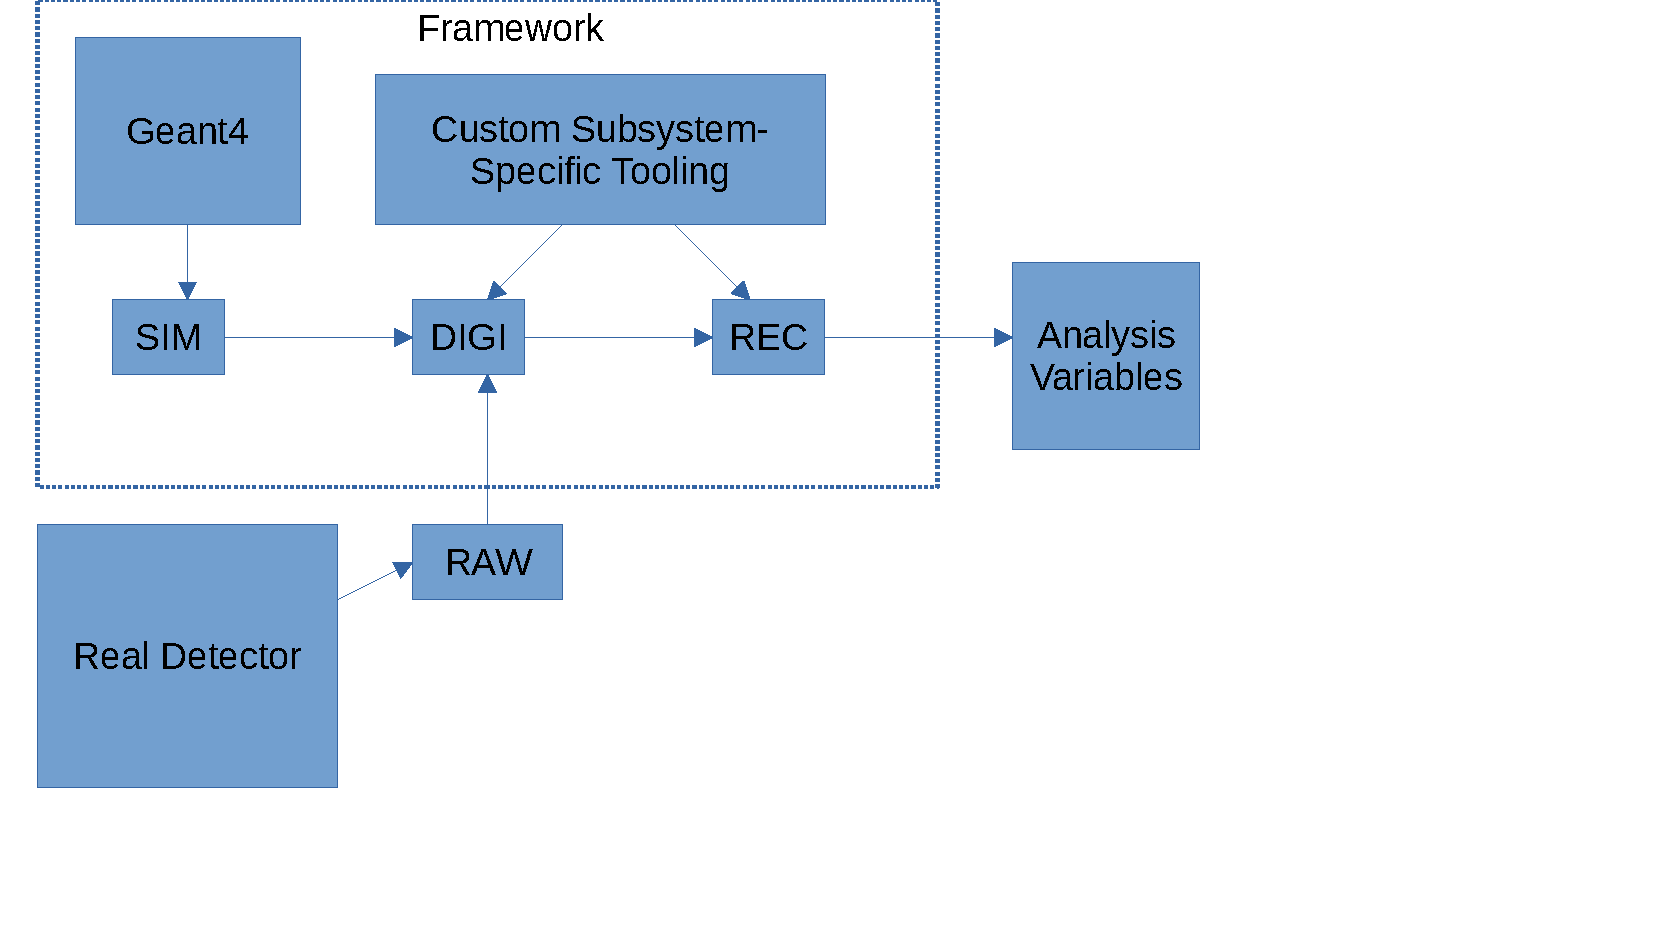
\includegraphics[width=0.9\textwidth]{figures/ldmx/simulation/data-flow.pdf}
  \caption{Diagram of processing stages within \ac{ldmx} showing the external sources of data or software that are used in those stages as well as which stages are commonly done within the centralized processing framework.}
  \label{fig:ldmx:sim:data-stages}
\end{figure}

In this work (as the chapter title implies), we focus mainly on the detector simulation stage where
data\todo[reword]{Distinguish ``data'' in software from the ``data'' of the experiment. What's
  another word for data that isn't overloaded?} is randomly generated in a way geared towards
realistically modeling the detector and particles interacting with it. The downstream stages,
namely electronic emulation and reconstruction, are not described further here; however, it should
be emphasized that all subsystems of \ac{ldmx} have their own custom implementations of these
stages in order to realistically emulate and reconstruct the data within their subsystem.

\subsection{Biasing and Filtering Technique}
Many of the processes most interesting for a \ac{dm} search within \ac{ldmx} are rare relative to
processes that are ``easier'' to reject by normal data processing.
In many cases, the rarity of these more interesting processes is a computational roadblock
since waiting for the entire detector simulation to complete before looking for these processes
of interest wastes a lot of computer time when only one out of every ten thousand events actually
contains a process we are interested in.
To make simulation of these processes more computationally feasible, we turn to the common simulation
techniques of biasing (artificially increasing the probability of a certain process occurring) and
filtering (ending the simulation of events if certain criteria are not met).

In the \ac{eat} analysis channel, all of our interesting processes occur within the developing
shower of particles in the \ac{ecal}.
While more complicated that checking for proceesses happening to the single beam electron,
we can enable looking for specific processes ocurring within this shower in a computationally
efficient way be tuning the order with which the simulation processes particles.
The detector simulation is focused only on particle-material interactions, so the order 
in which particles are simulated does not change how the physics is modeled.
We choose to process particles in two groups -- ``high'' and ``low'' energy --
where the high-energy particles are all processed before the low-energy particles.
The border between these two (called the ``Sorting Threshold'') is configurable by the user and enables a specific function\footnote{
The \texttt{NewStage} function of any \texttt{STACKING} \texttt{UserAction}s. 
} to be called mid-shower after all of the high-energy particles are processed
(i.e. simulated until their total energy falls below the Sorting Threshold).

Suppose we know from studying other (unbiased or low-bias) samples that showers need to have
a minimum amount of energy ``going into'' a specific process of interest before the shower
becomes ``important.''
We can set this minimum energy (here called the ``Filtering Threshold'') as a requirement on
the \ac{ecal} shower for the simulated event to be kept within the sample and, in order to
improve the speed of the filtering, we can apply this requirment \emph{during} the simulation
when the event transitions from the high-energy group to the low-energy group of particles.


Now, this infrastructure of determining a minimum simulated energy and having an energy-based
sorting of the processing order already helps improve the computational efficiency of these 
simluation samples (from $\sim 6$k CPU-hours to $\sim 30$ CPU-hours for $\sim 1$B EoT equivalent); 
nevertheless, it is still extremely slow and so we add biasing in order to artificially increase 
the rate of the process we wish the sample to focus on.
Since the processes we are interested in biasing are connected to particles that are abundant
within the electromagnetic \ac{ecal} shower, we need to require only particles above a
certain energy threshold (the ``Biasing Threshold'') to avoid over-sampling of the process.
In addition, we also need to define the factor that we will multiply the cross section by
when a particle is above the Biasing Threshold and in the \ac{ecal} volumes (the ``Biasing Factor'').

Artificially increasing the rate of a process relative to its true rate measured in nature
is obviously unphysical, but we can account for this by weighting the events depending on this
Biasing Factor when counting them.
The simulation engine we use does this weight calculation for us and it accounts for both the
biasing factor (beginning the weight with a factor of $1/B$) and unbiased processes happening
to a particle with biasing enabled (increasing the event weight to reflect that physical processes
at the natural rate have ocurred)

\begin{table}[htb]
    \centering
    \begin{tabular}{c|cc|p{0.4\textwidth}}
        Parameter & Dimension & Symbol & Short Description \\ \hline \hline
        Sorting Threshold & Energy & $T_S$ & Minimum total energy to be processed in first group \\ \hline
        Biasing Threshold & Energy & $T_B$ & Minimum total energy for a particle to be biased \\ \hline
        Biasing Factor & Dimension-less & $B$ & Factor to multiply cross section by \\ \hline
        Filtering Threshold & Energy & $T_F$ & Minimum energy transfered into a process for the event to be kept \\
    \end{tabular}
    \caption{Parameters of mid-shower biased samples. In all of the samples used in this study, we use the same value for the Sorting and Biasing Thresholds.}
    \label{tab:biasing-parameters}
\end{table}

Table \ref{tab:biasing-parameters} summarizes the parameters related to this
sample generation technique.
Practically, we choose to have the Biasing and Sorting Thresholds share the same value for all
of the samples in this work in order to reduce the number of parameters needed to tune and
to process all of the biased particles (as well as particles of similar energies
but different flavors) before making any filtering decision.

Generally, validation of this biasing and filtering technique can be done by checking that
the samples generated with this technique match samples generated without this technique
and with the filtering applied after the fact.
This validation needs to be done on a per-sample basis since the specific aspects of
the simulation that need to align may change depending on the specific physics
for which we are biasing and filtering.

\section{Standard Processes}
As displayed in \cref{fig:ldmx-bkgd-staircase}, there are a few categories of physics processes
that are described by the standard model and we expect to happen within our experiment. These
``background'' processes -- while interesting for other analyses of \ac{ldmx} data -- should be
rejected by this search for \ac{dm} since they are understood to \emph{not} be \ac{dm} by the
standard model and other experiments. In order to thoroughly and faithfully estimate our ability to
reject these backgrounds, we need to realistically simulate them within our detector volume.

\textsc{Geant4} \cite{geant4} has been developed for precisely this purpose. This study uses a slightly modified copy of \textsc{Geant4} v10.2.3 which focuses on improving the accuracy of processes relevant to a \ac{dm} search within \ac{ldmx} with the following needs.
\begin{enumerate}
  \item Updating cross section and sampling of $\gamma\to\mu^+\mu^-$ process to align it better with
        collected data and calculations of the standard model.
  \item Update nuclear cascade to align with more recent CLAS data specifically focused on the rate of
        low-multiplicity forward neutrons (Appendix A.A of \cite{ldmx-whitepaper}).
  \item Introduction of \emph{back scattering} $\pi^0$ in a $\gamma p \to \pi^0 p$ within a nuclear cascade
        (Appendix A.B of \cite{ldmx-whitepaper}).
\end{enumerate}
These updates enabled us to efficiently study the known and expected background processes interactions with the \ac{ldmx} detector design and compare this data to simulations of a model of a \ac{dm} production process.

\subsection{Dominate Contributors in this Analysis}
Generally, we focus on processes that would cause the energy in the \ac{ecal} to be
estimated at a significantly smaller value than the known beam energy.
This ``missing'' energy is used as a key piece of evidence that the event in question
should be stored for further study and thus is the main ingredient in the infrastructure
deciding whether a specific event should be stored (the ``trigger'').
From prior experience with \ac{ldmx} (e.g. \cite{ldmx-whitepaper,ldmx-photon-reject-2020}),
we expect certain types of standard processes to dominate the backgrounds that pass this
trigger requirement on missing energy: interactions with the nuclei of the detector
material producing hard-to-detect hadrons (so-called ``nuclear'' processes) and conversion
of photons into a pair of muons (which are also difficult for the \ac{ecal} to detect).

Nevertheless, we still can use a large, unbiased simulation sample in order to verify
these previous conclusions and inform our decisions on how the subsequent biased samples
should be produced.
\cref{fig:rec-efrac-by-nuc} is a key piece of evidence along these lines
where we separate the total reconstructed energy (the estimate from our detector)
as a fraction of the known beam energy by the amount of energy going into these nuclear
processes (so-called ``nuclear'' energy).
We see that as more energy is given to these nuclear interactions,
the reconstructed fraction decreases.
Eventually, we reach a point where enough energy has gone to these nuclear interactions
that we expect the event to be below the trigger threshold and be kept by the trigger
system at a significant rate.

\begin{figure}
  \centering
  \begin{tabular}{cc}
    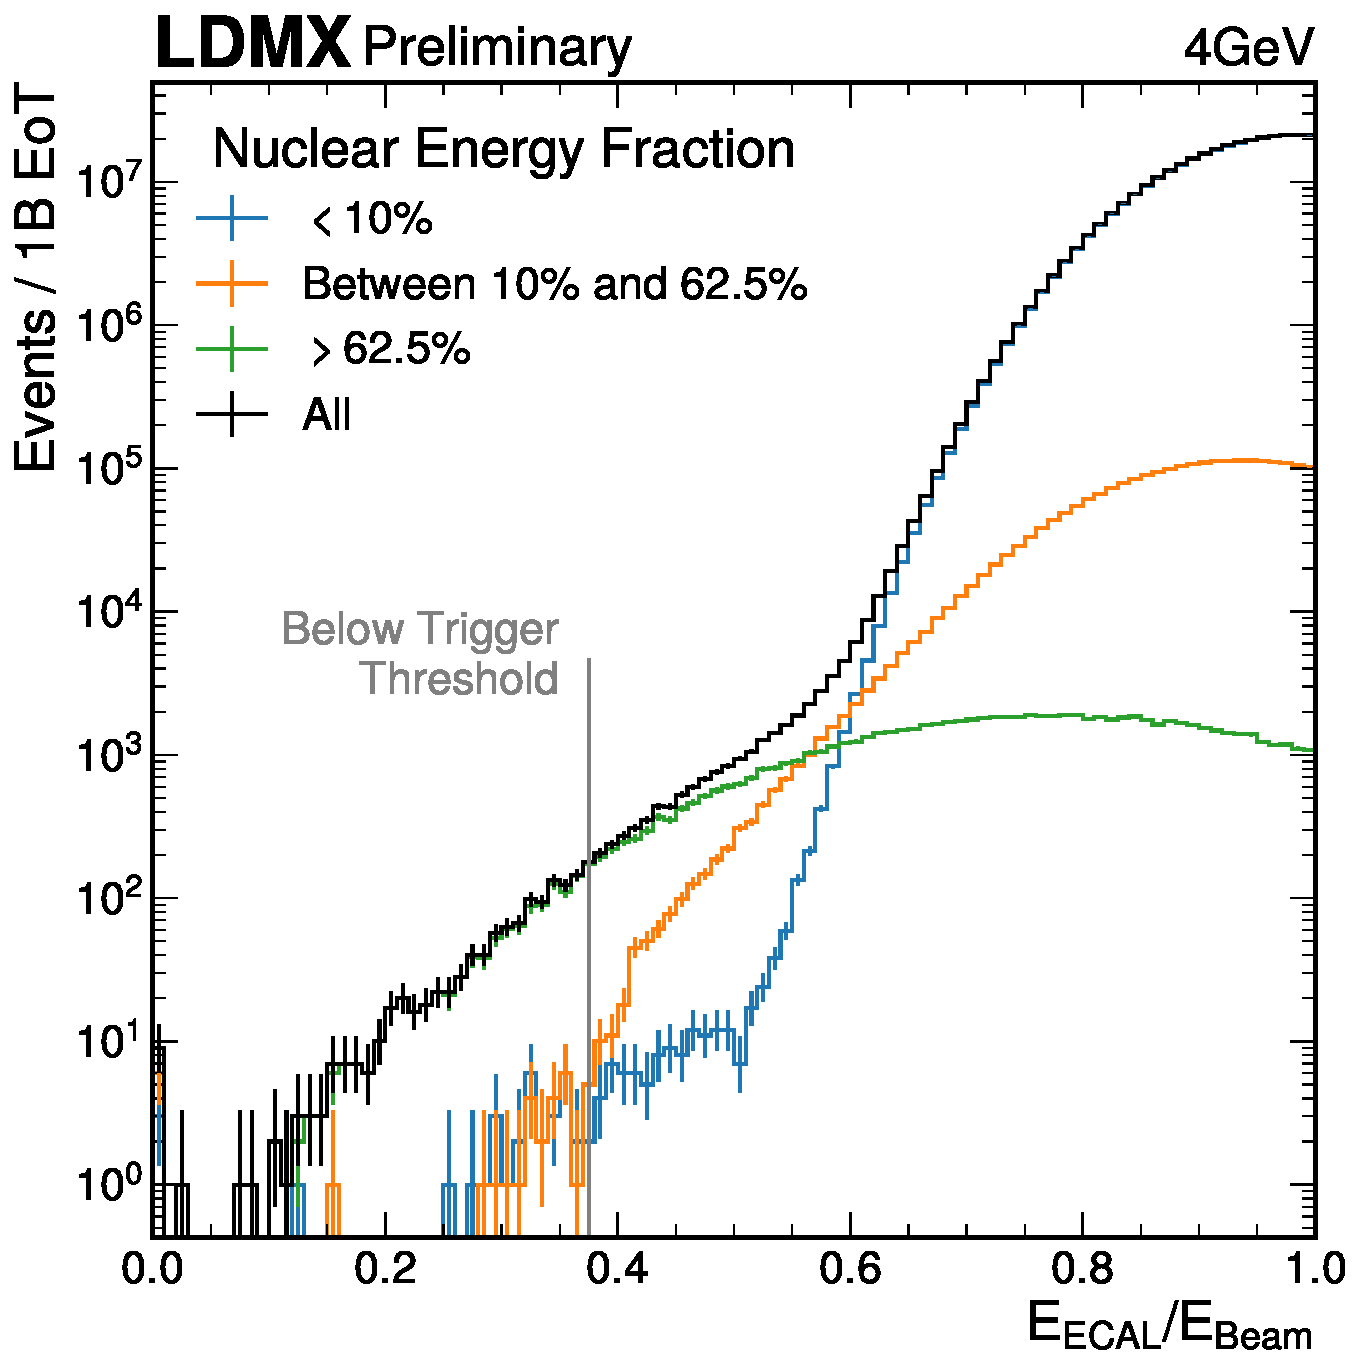
\includegraphics[width=0.49\textwidth]{figures/ldmx/simulation/4gev-ecal-by-nuc.pdf}
    &
    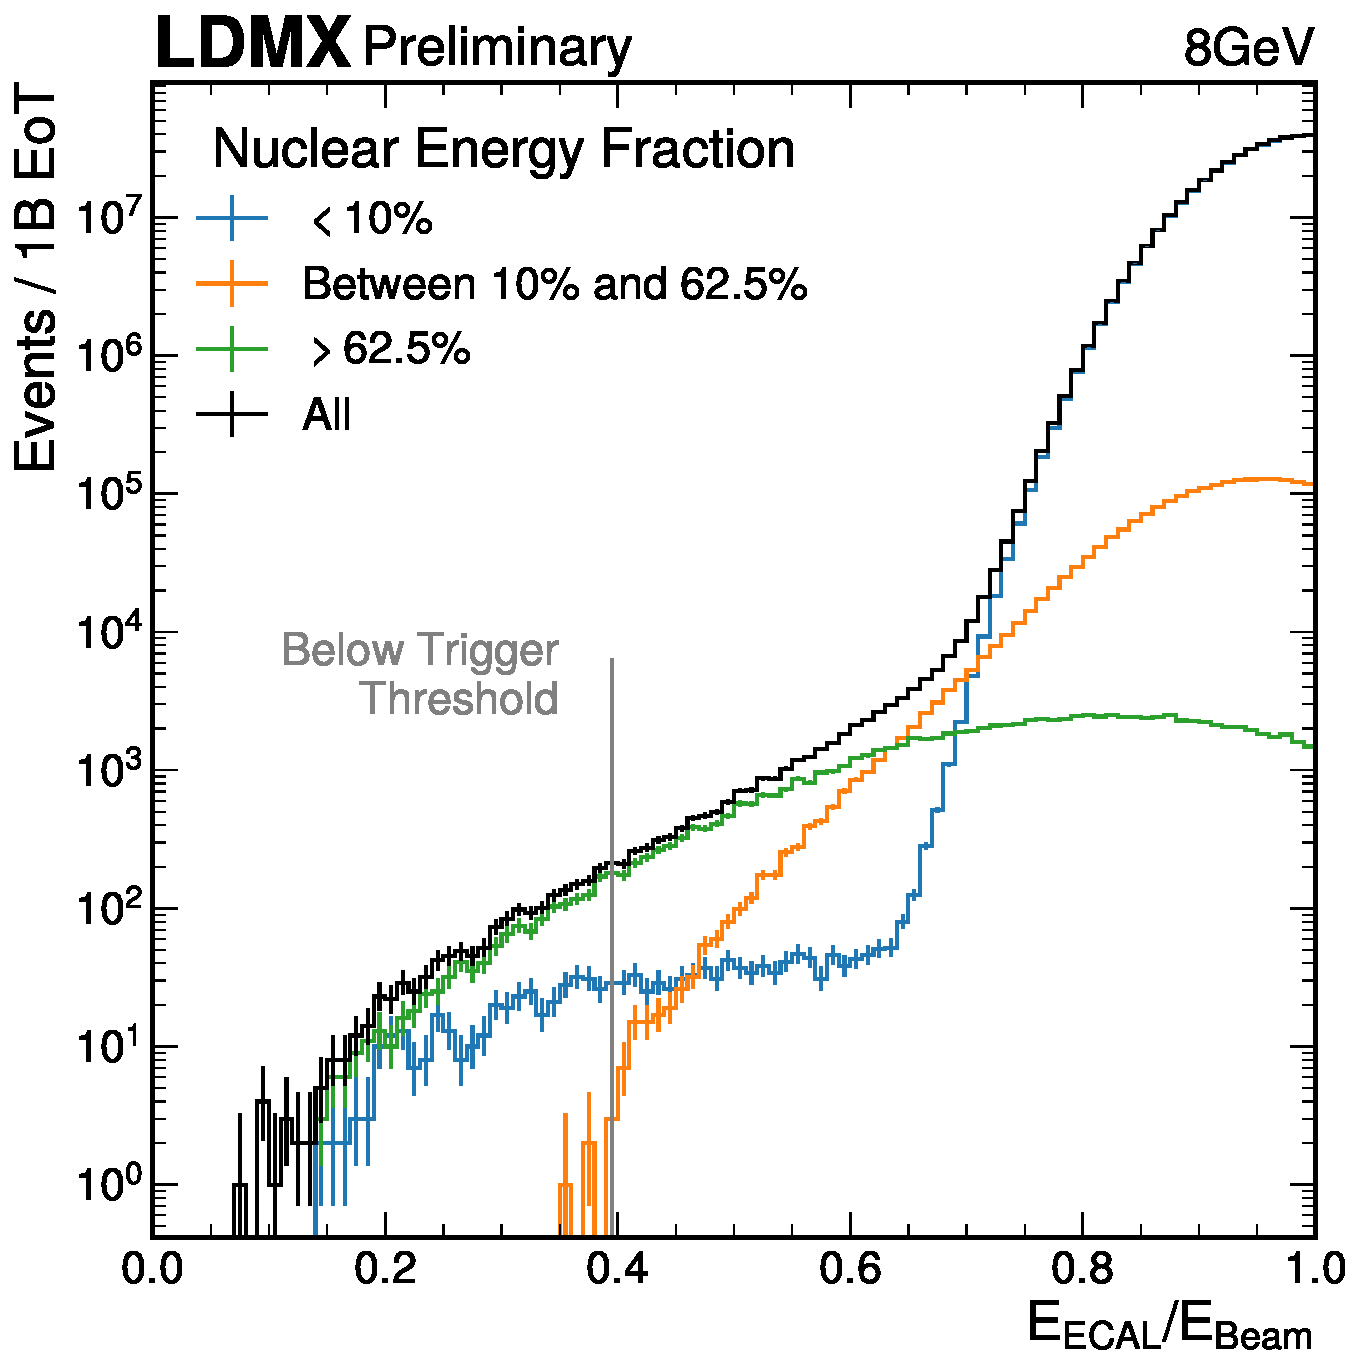
\includegraphics[width=0.49\textwidth]{figures/ldmx/simulation/8gev-ecal-by-nuc.pdf}
  \end{tabular}
  \caption{The total reconstructed energy within the \ac{ecal} as a fraction of the beam energy
  separated by the total nuclear energy within the event (the energy going into the photon-nuclear
  and electron-nuclear processes).}
  \label{fig:rec-efrac-by-nuc}
\end{figure}

\cref{fig:rec-efrac-by-nuc} shows that a significant fraction of events whose total nuclear
energy is greater than \qty{62.5}{\percent} of the beam energy fall below the threshold for
the trigger.
This figure also shows that there are other types of events that do not have much (if any)
nuclear interactions (since their nuclear energy is less than \qty{10}{\percent} of the beam
energy) but still are reconstructed below the trigger threshold.
\todo[dimuon]{insert dimuon plot to show that these other events are dimuon events}

\subsection{Expanding Production of these Processes}
\todo[copy]{Copy background sample validation appendices from EaT internal note.}

\section{Dark Matter Signal}
The particular signal process this analysis channel is looking for is the production of a dark
photon followed by an \emph{invisible} decay. In this regime, what happens to the dark photon after
it is produced is irrelevant to the analysis since both it and its products are not observable by
our detector.

With this focus in mind, we developed a dark bremsstrahlung simulation method that allows for the
visible particle (the recoiling lepton) to be distributed according to a full matrix element
calculation (via MG/ME) while the incident particle can have varied energy and be handled by Geant4
directly. This novel simulation technique allows for the dark bremsstrahlung process to be treated
(from Geant4's perspective) on the same footing as the background processes while maintaining the
precision of a matrix-calculator method.

\subsection{G4DarkBreM}
To accurately simulate the kinematics of the dark bremsstrahlung process for electrons in thick
targets, the process must be included at the level of experimental simulation instead of using
initial state event generators to account for the possibility of energy loss through bremsstrahlung
or multiple scattering prior to the dark matter interaction. Accurate kinematic simulation of the
outgoing electron are required for optimal experimental sensitivity measurements and appropriate
design of search strategies.

For this reason, we utilize G4DarkBreM \cite{g4darkbrem} which performs this embedding of the dark
bremmstrahlung process into \textsc{Geant}4. G4DarkBreM calculates the cross section using
numerical integrals of the Weizs\"{a}cker-Williams approximation, and the kinematics are simulated
using a scaling technique of \textsc{MadGraph/MadEvent} event libraries. The accuracy of the total
cross section and kinematics is validated using \textsc{MadGraph/MadEvent} samples at a range of
incident lepton energies.

\subsection{MadGraph/MadEvent}
For this study in \ac{ldmx}, the code package used to develop and validate G4DarkBreM was also used
to generate the input refernece libraries for sample generation. This code is a custom version of
\textsc{MadGraph/MadEvent4} with the following updates.
\begin{itemize}
  \item Introduction of basic dark sector particles (massive boson and spin-$1/2$ fermion) which act as the
        representatives of the dark sector interacting with the standard model particles.
  \item Definition of a nuclear particle (electrically neutral, spin-$1/2$ fermion) with new couplings to
        the dark photon including the nuclear form factors.
  \item Updating the definition of the electron to include its small (but non-zero) mass to prevent
        divergence of the cross section at lower energies.
\end{itemize}
These updates, along with some wrapping code, enables the generation of
dark bremmstrahlung events for a range of target nuclei, incident energies,
and either incident electrons or muons.

As suggested by the validation of G4DarkBreM \cite{g4darkbrem}, we generate libraries where the
incident electron's energy drops in steps of 10\% down from the beam energy. Since the dark photon
is required to be simulated with at least 50\% of the beam energy, we stop the library generation
also at 50\% of the beam energy. The primary nuclei that could dark brem within the \ac{ecal} are
tungsten, silicon, oxygen, and copper so those are the nuclei for which we generate libraries. The
rest of the nuclei within the simulated \ac{ecal} (sodium, calcium, carbon for example) have atomic
numbers close to those nuclei already sampled and so can be faithfully simulated with these
libraries. In order to avoid duplicating the same event, a unique reference library is generated
for each simulation run even when keeping the dark photon mass and beam energy the same.

\subsection{Characterization}
Describe how these samples "look"?

%%%%%%%%%%%%%%%%%%%%%%%%%%%%%%%%%%%%%%%%%%%%%%%%%%%%%%%%%%%%%%%%%%%%%%%%%%%%%%%%

%%%%%%%%%%%%%%%%%%%%%%%%%%%%%%%%%%%%%%%%%%%%%%%%%%%%%%%%%%%%%%%%%%%%%%%%%%%%%%%%
% After generating data, what we do to select signal and prepare for search
%%%%%%%%%%%%%%%%%%%%%%%%%%%%%%%%%%%%%%%%%%%%%%%%%%%%%%%%%%%%%%%%%%%%%%%%%%%%%%%%
\chapter{Analysis}
\label{chapter:ldmx:analysis}
%%%%%%%%%%%%%%%%%%%%%%%%%%%%%%%%%%%%%%%%%%%%%%%%%%%%%%%%%%%%%%%%%%%%%%%%%%%%%%%%

The \ac{eat} analysis channel for \ac{ldmx} has two primary purposes which can
be separated by the timeline over which they are relevant.
\begin{enumerate}
	\item \textbf{Short Term}: In early running, when the number of \ac{eot} is
	      relatively small, the nominal \ac{mm} analysis will not have obtained
	      significant reach into new \ac{dm} phase space (yet). The \ac{eat} channel
	      serves here as a way to obtain world-leading sensitivity early in the lifetime
	      of \ac{ldmx} and give the collaboration a first look at the data the apparatus
	      has collected.
	\item \textbf{Long Term}: As \ac{ldmx} collects data, the \ac{mm}
	      analysis enters into unexplored phase space and serves as a better discovery
	      mechanism due to its access to the Tagger and Recoil trackers. The \ac{eat}
	      channel, while struggling to suppress complicated backgrounds with relatively
	      limited analysis handles, can operate ``orthogonally'' in the collected data
	      since its primary selection (an approximately beam-energy electron passing
	      through the Recoil tracker) is inverted relative to the \ac{mm} analysis
	      (the electron passing through the Recoil tracker has significantly less
	      energy than the beam).
\end{enumerate}
As a first investigation of the \ac{eat} analysis channel, this work is focused on
the first (short term) purpose. In this regard, we target an \ac{eot} that is reasonable
to accomplish early in the running of \ac{ldmx} and avoids particularly intricate backgrounds.
\num{1e13} \ac{eot} fits these requirements by avoiding the charged current production
of neutrinos and represents $\sim\qty{10}{percent}$ of the first full \ac{ldmx} dataset.
obtainable within approximately a week of beam time\footnote{
	Assuming the \ac{ldmx} detector apparatus and beam delivery is operating according to specifications, we expect the beam to be delivered on a frequency of \qty{37.5}{\mega\hertz} with a duty cycle of $\approx$\num{0.5}.
	$\qty{37.5}{\mega\hertz}\times0.5\times\qty{1}{week}\approx\num{1.1e13}$~\ac{eot}.
}.
Since \ac{eat} is expected to be the \emph{first} physics
analysis on \ac{ldmx} data, we want a \emph{simple} and \emph{robust} analysis that can withstand
the test of time and the complexities of real data.

With these design goals in mind, a simple ``cut-and-count'' analysis has been developed.
The simplicity of this analysis is one of its strengths, enabling it to be applicable
despite potential surprises arising from first encounters with real data.
The bulk of time and effort on this first investigation was focused on making this
investigation \emph{possible} via the introduction of midshower process filtering
and a dark bremsstrahlung simulatin process described in \cref{chapter:ldmx:simulation}.

\section{Trigger}
Use same on-line trigger as MM analysis.

Re-apply trigger threshold to entire ecal energy sum off-line (same as MM analysis)

\section{Cut and Count}
List cuts for different beams, provide final background yields and signal efficiencies.

\section{Reach}
Display reach of ME analysis with different background hypotheses and signal efficiencies
motivated by findings above.

%%%%%%%%%%%%%%%%%%%%%%%%%%%%%%%%%%%%%%%%%%%%%%%%%%%%%%%%%%%%%%%%%%%%%%%%%%%%%}}}


\part{HPS} \label{part:hps}
%%%%%%%%%%%%%%%%%%%%%%%%%%%%%%%%%%%%%%%%%%%%%%%%%%%%%%%%%%%%%%%%%%%%%%%%%%%%%%%%
% experiment.tex: Chapter describing the experiment
%%%%%%%%%%%%%%%%%%%%%%%%%%%%%%%%%%%%%%%%%%%%%%%%%%%%%%%%%%%%%%%%%%%%%%%%%%%%%%%%
\chapter{Heavy Photon Search}
\label{chapter:hps:experiment}

\acf{hps} is a fixed-target experiment currently in operation at \ac{jlab}
which is focused on search for short-length (few centimeter) decays of new particles.
In order to search for these visible signatures of new particles,
\ac{hps} must be able to precisely reconstruct the produced \ac{sm} particle
kinematics and then use this information to estimate their origin point (their
``vertex'').
This reconstruction is enabled by two key detector components whose design
will be motivated using the model studied in more detail in this part.

\section{Strongly Interacting Massive Particles}
\label{sec:hps:simps}

As mentioned in \cref{sec:theory:visible}, our search for \ac{dm} must accomodate the possibility
that any \ac{dm} produced within our experiments subsequently decays back into \ac{sm} particles.
In order to model these types of \ac{dm}, we must account for both how the \ac{dm} is produced and
how it decays back to \ac{sm} particles. These theories propose new specific vertex rules for
constructing the Feynman diagrams and for the vertex factors within the calculations.

To be even more specific, we could hypothesize that the dark sector consists of particles that
interact with each other strongly in the same sense of the standard quarks. These Strongly
Interacting Massive Particles (SIMPs) \cite{simp-mechanism-2014,simp-pheno-2018} would then form
composite particles similar to how standard quarks form composite particles like protons and
neutrons. Since we expect our experiments to not reach the energies required to separate the
constiuents of these composite particles, the composite particles themselves would be the dark
matter candidates and the ones we represent within our diagrams. A dark sector consisting of SIMPs
would have a plethora of composite particles which we could observe; however of particular
importance is that there could be a composite particle that has similar enough properties to the
dark photon that it could ``mix'' with it and decay in a way that emits fewer dark particles:
\cref{fig:dark-brem-simp-decay}. This decay, since it has less energy ``lost'' to the dark
particles, has a greater potential of being observed within \ac{hps} and is discussed here.

\begin{figure}
  \centering
  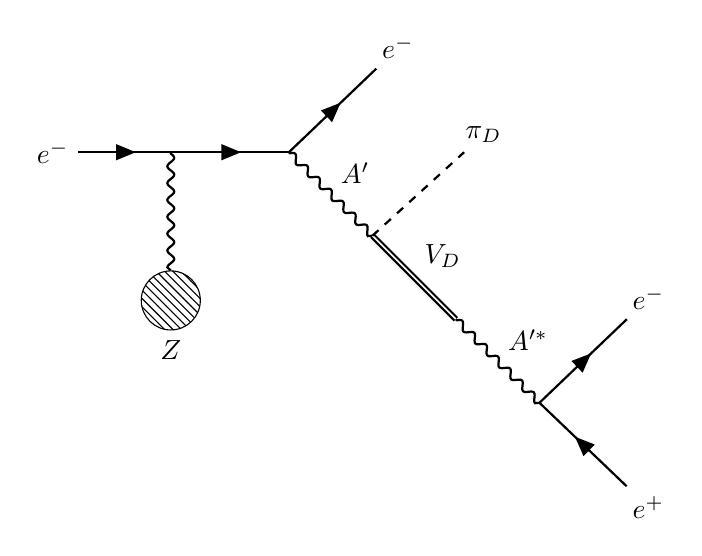
\begin{tikzpicture}
    \begin{feynman}
      \vertex (a) {$e^{-}$};
      \vertex [right= of a](d);
      \vertex [below=of d, blob,label={below:$Z$}] (e) {};
      \vertex [right= of d] (b);
      \vertex [above right= of b] (g) {$e^{-}$};
      \vertex [below right= of b] (aprime_decay);
      \vertex [below right= of aprime_decay] (rhod_decay);
      \vertex [above right= of aprime_decay] (dm) {$\pi_D$};
      \vertex [below right= of rhod_decay] (i);
      \vertex [above right= of i] (j) {$e^{-}$};
      \vertex [below right= of i] (k) {$e^{+}$};
      \diagram*[large] {
      (a) -- [fermion] (d),
      (d) -- [boson] (e),
      (d) -- [fermion] (b),
      (b) -- [fermion] (g),
      (b) -- [boson, edge label={$A'$}] (aprime_decay) -- [double, edge label={$V_D$}] (rhod_decay),
      (aprime_decay) -- [scalar] (dm),
      (rhod_decay) -- [boson, edge label={$A'^*$}] (i),
      (k) -- [fermion] (i) -- [fermion] (j),
      };
    \end{feynman}
  \end{tikzpicture}
  \caption{
    Diagram of dark brem production of a dark photon followed by its decay back into an electron-positron pair
    through SIMP composite particle $V_D$ with the emission of a lighter SIMP composite particle $\pi_D$.
    The two-particle vertex $V_D-A'$ is only allowed since they share enough quantum properties to mix.
  }
  \label{fig:dark-brem-simp-decay}
\end{figure}

Importantly, \cref{fig:dark-brem-simp-decay} has two vertices where \ac{dm} and \ac{sm} particles
interact -- these two vertices represent the fact that such a visible decay is subsequently less
probable since both of these vertices carry with them the weak mixing factor $\epsilon$. The lower
probability of these visible decays is a general property of such signatures and motivates
experiments focused on collecting large data volumes in order to overcome the limitation imposed by
this lower probability. With this in mind, \ac{hps} has been built to observe a beam whose rate is
significantly high -- high enough to prevent sensitive detector elements from being placed directly
within its path.

The observable outgoing particles of \cref{fig:dark-brem-simp-decay} can be mimiced by existing
\ac{sm} processes. The most prominent background process is trident production \cref{fig:trident}
which enables the production of the electron-positron pair through the radiation of the virtual
photon (\cref{fig:trident:radiative}) or through direct electromagnetic interaction with the
nucleus and a virtual lepton (\cref{fig:trident:bethe-heitler}). The upside of this trident
production process is that it is \emph{prompt} -- i.e. the produced electron and positron originate
from within the target. The position of this vertex is a separation from the signal process
\cref{fig:dark-brem-simp-decay} where the vertex of the produced electron and positron would be
observably displaced downstream of the target due to the non-zero lifetime of the dark sector
particle $V_D$.

\begin{figure}
  \centering
  \begin{subfigure}[t]{0.4\textwidth}
    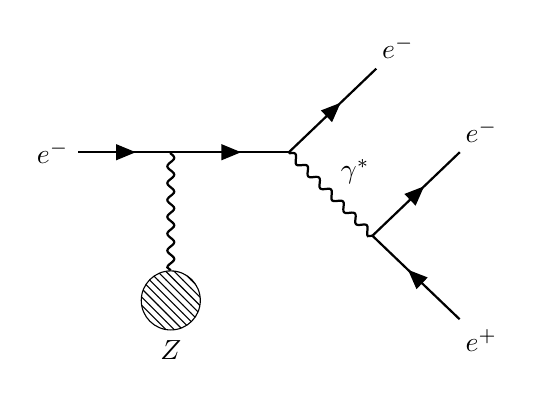
\begin{tikzpicture}
      \begin{feynman}
        \vertex (a) {$e^{-}$};
        \vertex [right= of a](d);
        \vertex [below=of d, blob,label={below:$Z$}] (e) {};
        \vertex [right= of d] (b);
        \vertex [above right= of b] (g) {$e^{-}$};
        \vertex [below right= of b] (rad);
        \vertex [above right= of rad] (j) {$e^{-}$};
        \vertex [below right= of rad] (k) {$e^{+}$};
        \diagram*[large] {
        (a) -- [fermion] (d),
        (d) -- [boson] (e),
        (d) -- [fermion] (b),
        (b) -- [fermion] (g),
        (b) -- [boson, edge label={\(\gamma^*\)}] (rad),
        (k) -- [fermion] (rad) -- [fermion] (j),
        };
      \end{feynman}
    \end{tikzpicture}
    \caption{Radiative trident}
    \label{fig:trident:radiative}
  \end{subfigure}%
  ~
  \begin{subfigure}[t]{0.4\textwidth}
    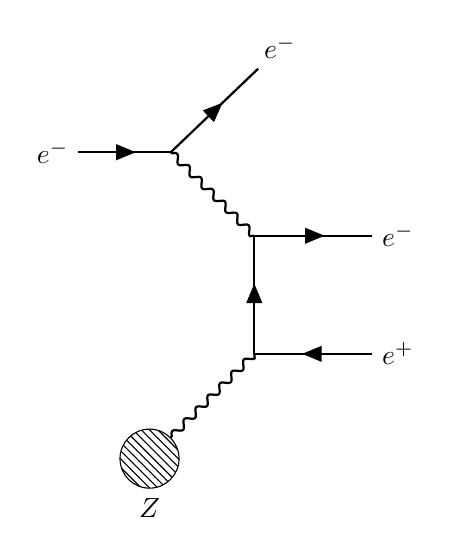
\begin{tikzpicture}
      \begin{feynman}
        \vertex (a) {$e^{-}$};
        \vertex [right= of a] (d);
        \vertex [above right= of d] (g) {$e^{-}$};
        \vertex [below right=of d] (eleprod);
        \vertex [below=of eleprod] (posprod);
        \vertex [right=of eleprod] (j) {$e^{-}$};
        \vertex [right=of posprod] (k) {$e^{+}$};
        \vertex [below left=of posprod, blob,label={below:$Z$}] (e) {};
        \diagram*[large] {
        (a) -- [fermion] (d) -- [fermion] (g),
        (d) -- [boson] (eleprod),
        (e) -- [boson] (posprod),
        (k) -- [fermion] (posprod) -- [fermion] (eleprod) -- [fermion] (j),
        };
      \end{feynman}
    \end{tikzpicture}
    \caption{Bethe-Heitler trident}
    \label{fig:trident:bethe-heitler}
  \end{subfigure}
  \caption{Feynman diagrams for the \ac{sm} process of trident production.}
  \label{fig:trident}
\end{figure}

\ac{hps} is designed to focus on visible signatures of \ac{dm} like SIMPs with
a dual strategy of searching for mass resonances and displaced vertices.
Both of these strategies require high data volume and precise reconstruction of a produced
electron-positron pair originating from the decay of some \ac{dm} particle.
The precision of this reconstruction is one of the main limiting factors in distinguishing
whether a specific pair originated from \ac{dm} or from some other \ac{sm} background process.
These design drivers have led to the the apparatus discussed below.

\section{Detector Apparatus}
%%%%%%%%%%%%%%%%%%%%%%%%%%%%%%%%%%%%%%%%%%%%%%%%%%%%%%%%%%%%%%%%%%%%%%%%%%%%%%%%
\ac{hps} is currently installed behind the CLAS-12 experiment in the Hall B
alcove at \ac{jlab} and utilizes the \ac{cebaf} to provide its beam
\cite{mrsolt-thesis-2020,skmccarty-thesis-2020}.
Hall B primarily hosts the CLAS-12 experiment in the bulk of its hall; nevertheless,
behind the CLAS-12 experiment \ac{hps} is situated
within an alcove such that it can collect data whenever CLAS-12 is not operational (for example,
when its components are being upgraded or fixed).

\ac{cebaf} \cite{cebaf-12GeV-2012,cebaf-opportunities-2012,cebaf-2013} is able to
provide a near-continuous electron beam ranging in energy up to $12$ GeV in steps
of $\approx 1.15$ GeV. \ac{cebaf} is built in a oval ``race track'' where the straight
portions consist of linear accelerators and the curve portions steer the beam with
dipole magnets either back into the straight portions or into experimental halls.
Since \ac{cebaf} delivers electrons at such a high rate, \ac{hps} must be able to
handle these high radiation loads. Designed to be a small experiment to fit within
the Hall B alcove, \ac{hps} elected to be built in two halves that straddle the primary
path of the beam where the highest amount of radiation would be. Both of the subsystems
within \ac{hps} are split into these two halves as shown in \cref{fig:hps-full-render}
and \cref{fig:hps-diagram}.

\begin{figure}
  \centering
  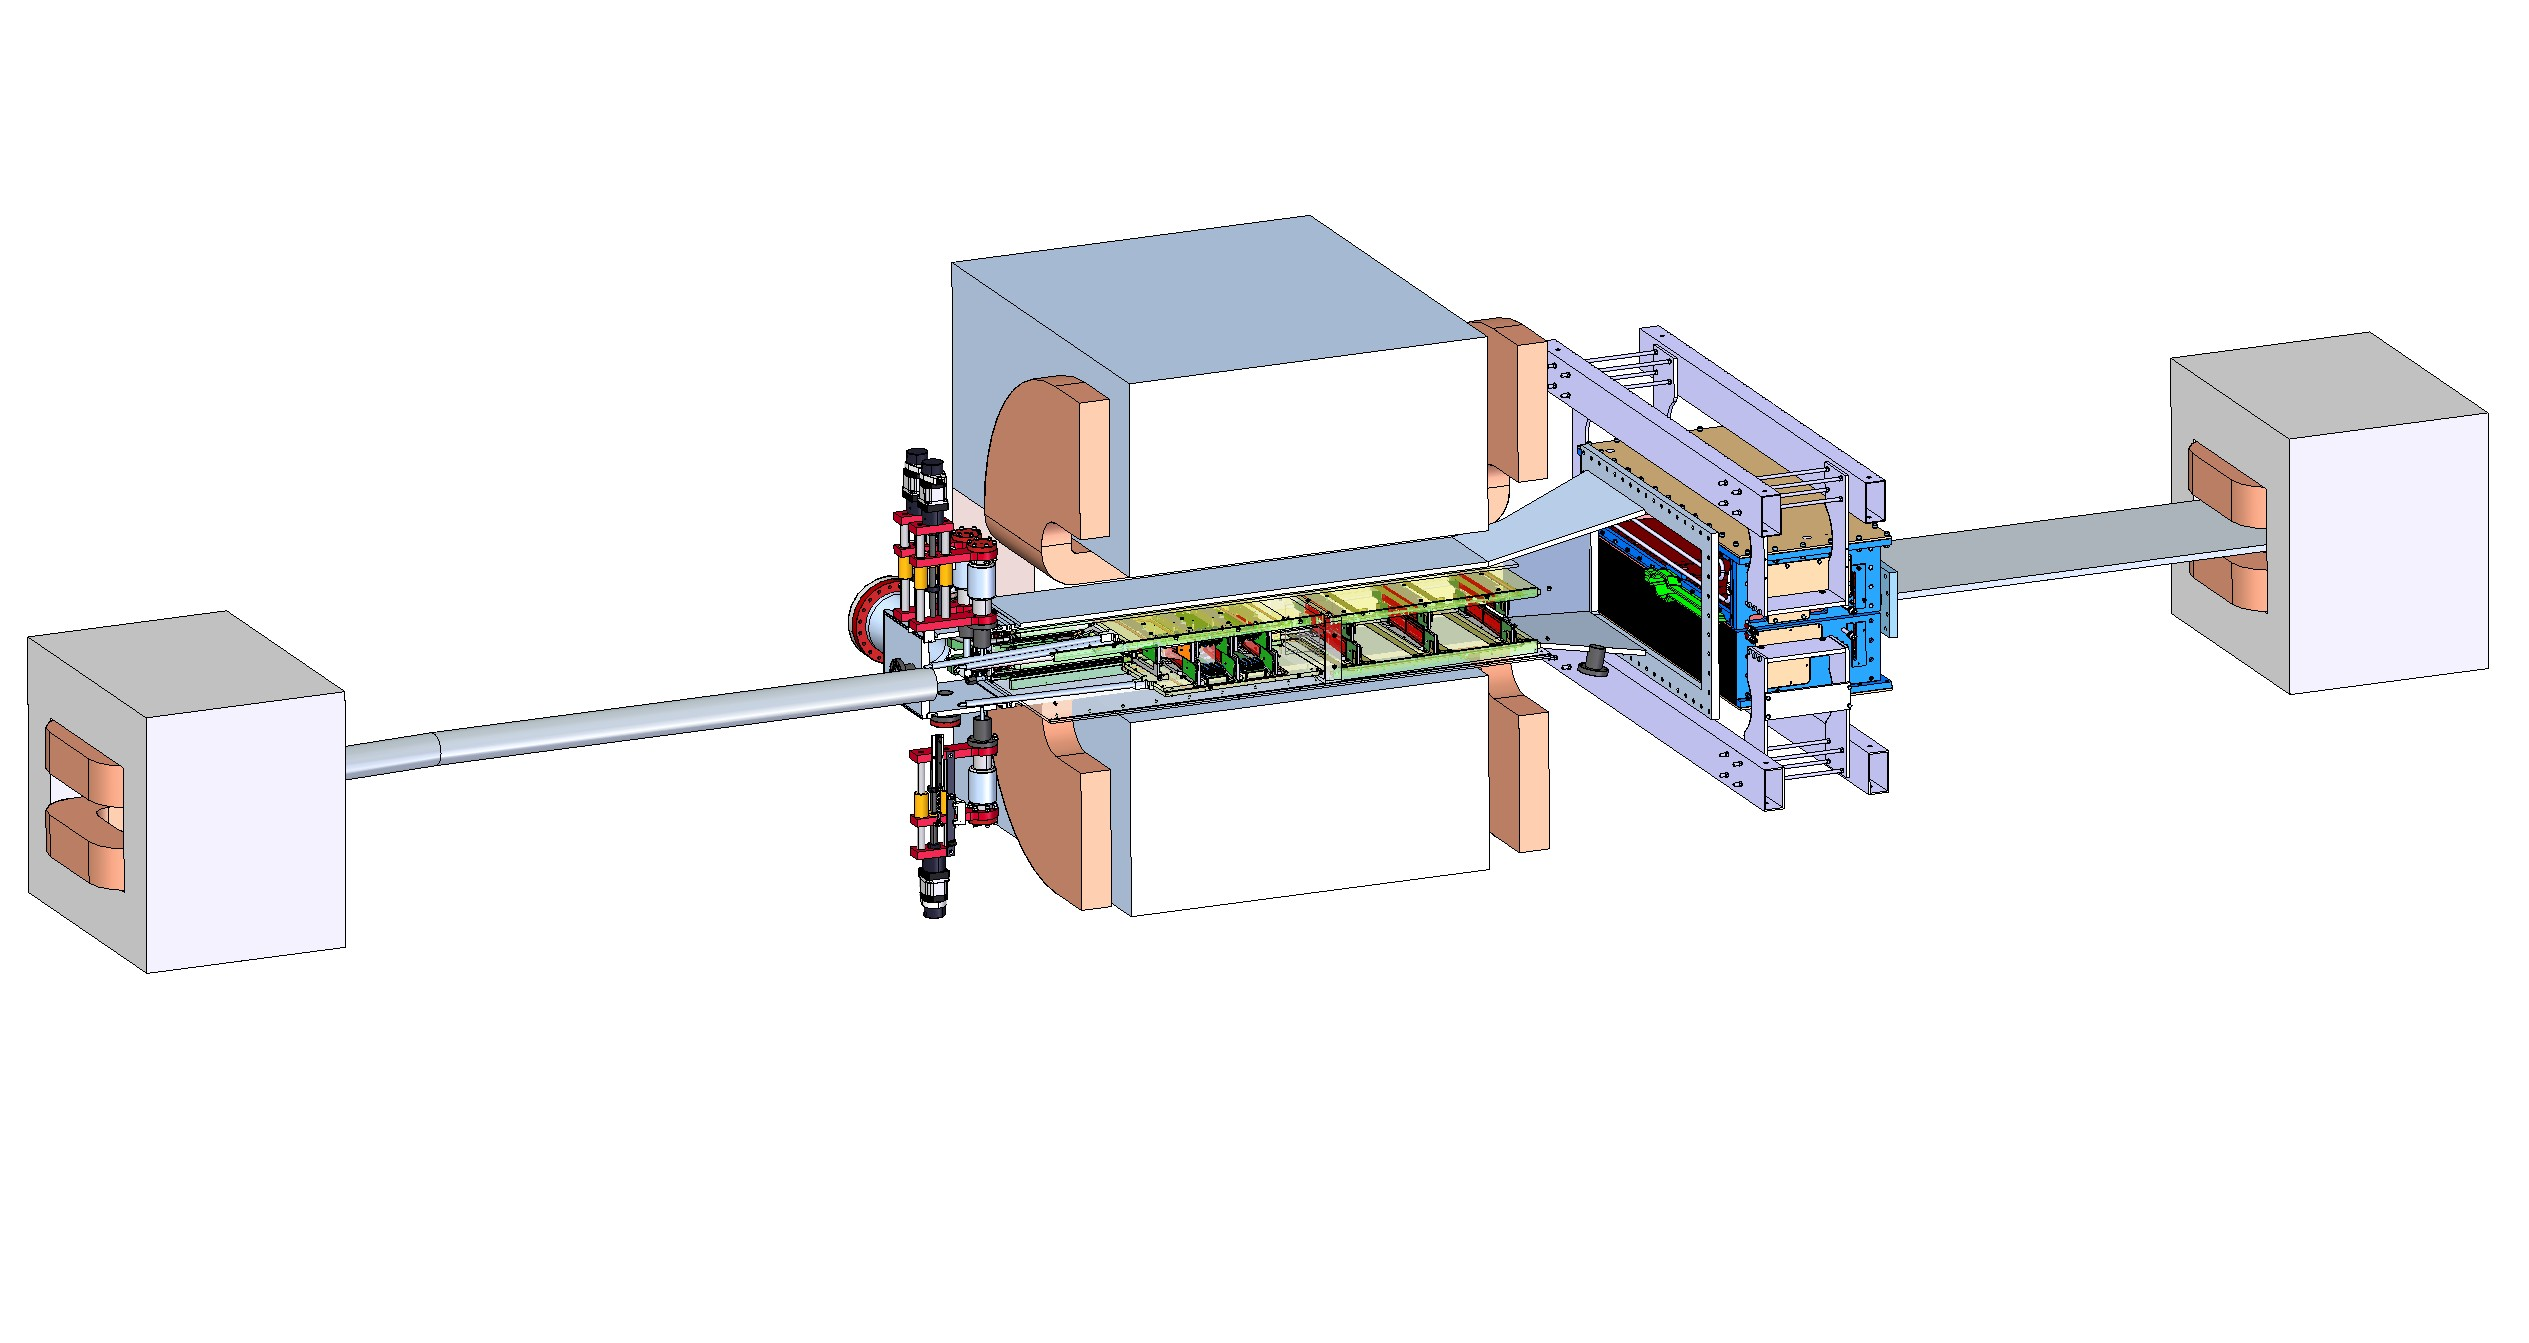
\includegraphics[trim={15cm 10cm 10cm 5cm},clip,width=\textwidth]{figures/hps/experiment/hps_full_render.jpg}
  \caption{
    Full rendering of \ac{hps}.
    Beam would enter the detector from the left and exit to the right if it does not interact.
  }
  \label{fig:hps-full-render}
\end{figure}

\begin{figure}
  \centering
  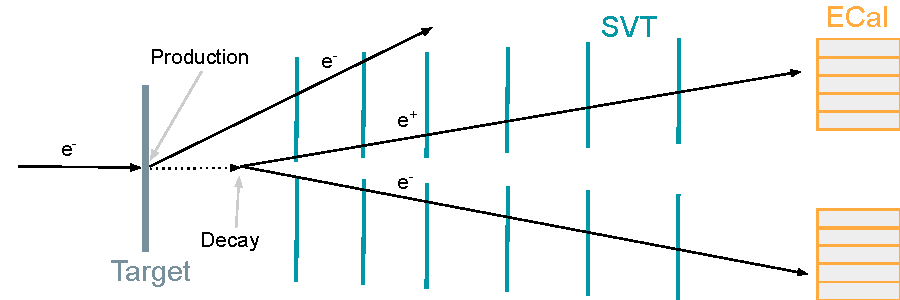
\includegraphics[width=0.9\textwidth]{figures/hps/experiment/hps-diagram.pdf}
  \caption{
    Simplified diagram of \ac{hps} showing an example displaced decay within the named subsystems.
    Not to scale.
    The dotted, unlabeled arrow is some \ac{dm} candidate particle that has a macroscopic lifetime causing
    the decay vertex to be observably displaced from the production within the target.
  }
  \label{fig:hps-diagram}
\end{figure}

The two subsystems included within \ac{hps} are the \ac{svt} focused on reconstruction of the
momentum and charge of charged particles and the \ac{ecal} focused on energy reconstruction and
online triggering of the data.

\subsection{Silicon Vertex Tracker}
The \ac{svt} is made of eighteen modules each of which is a pair of silicon-strip detectors offset
from each other by a small angle to enable three-dimensional position reconstruction. The modules
are arranged in the two halves separated by the center beam line. In each half, the modules are put
into layers with the first three layers consisting of one module while the last three layers
consisting of two modules to increase angular acceptance relative to the target.
\cref{fig:hps-svt-render} shows a rendering of the \ac{svt} with the sensitive detector elements
shown as red rectangles.\footnote{ This diagram and the description within this thesis is focused
  on the \ac{hps} \ac{svt} from its physics run in 2016. Various \ac{hps} components have been
  upgraded for subsequent runs. }

The two halves of the \ac{svt} are positioned to form a \qty{15}{\milli\radian} angular gap
relative to the target in order to avoid the largest amount of radiation from the beam. The first
layer (closest to the target, left size of \cref{fig:hps-svt-render}) is placed \qty{10}{\cm} from
the target and \qty{0.5}{\mm} from the beam line in order to maximize acceptance. The entire
\ac{svt} is enclosed in a vacuum box to limit secondary production of particles and is liquid
cooled to help prevent radiation damage.

The \ac{svt} modules are readout by APV25 chips which report six samples every \qty{24}{\ns}. These
samples are only dumped to disk upon receiving a trigger signal from the calorimter system
(\cref{sec:hps-ecal}).

All together, the \ac{svt} has been observed to have \num{10}~\% momentum resolution,
\qty{2.4}{\ns} time resolution, and \qty{6}{\micro\meter} position resolution. These properties
enable the necessary momentum and vertex reconstruction for \ac{dm} searches via visible decays.

\begin{figure}
  \centering
  \includegraphics*[width=\textwidth]{figures/hps/experiment/smkcarty-thesis-fig-10-svt-render.png}
  \caption{
    Figure 10 of \cite{skmccarty-thesis-2020}. Rendering of the \ac{svt} with the vacuum
    enclosure shown in gray, active silicon components in red, and readout electronics in
    green. Similar to \cref{fig:hps-full-render}, the beam would traverse this rendering
    from left to right.
  }
  \label{fig:hps-svt-render}
\end{figure}

\subsection{Electromagnetic Calorimeter}
\label{sec:hps-ecal}
The \ac{ecal} consists of \num{442} lead-tungstate crystals and is a fully-sensitive calorimeter.
The crystals are arranged in symmetric grids separated by the beamline similar to the \ac{svt}.
\cref{fig:hps-pair-trigger-depiction} shows this grid in addition to example clusters and \ac{ecal}-related
variables. In addition to a horizontal gap separating the halves, a few more crystals in the highest
radiation area are removed to form a ``hole'' to allow the majority of non-interacting (or minimally interacting)
beam electrons to pass through the detector volume. The calorimeter is sized to fit the same
angular acceptance as the \ac{svt} located \qty{139}{\cm} away from the target.

As mentioned above, one of the primary purposes of the \ac{ecal} is to be the triggering mechanism
for data collection. Many different trigger algorithms with different purposes have been used
within \ac{hps} and the specific trigger algorithm designed for collection of data relevant to a
\ac{dm} search is studied and motivated in detail in \cite{skmccarty-thesis-2020}.
\cref{fig:hps-pair-trigger-depiction} diagrams an event that would pass the pair-wise trigger used
for the collection of the data within this study. The trigger requirements include two
spatially-separated clusters of energy which are in separate vertical and horizontal halves of the
detector. These clusters must also have minimum energies of \qty{0.4}{\giga\electronvolt}
individually and total energy together of more than \qty{1}{\giga\electronvolt}. \todo[lookup]{get
  details of pair trigger used for the collected data.}

\begin{figure}
  \centering
  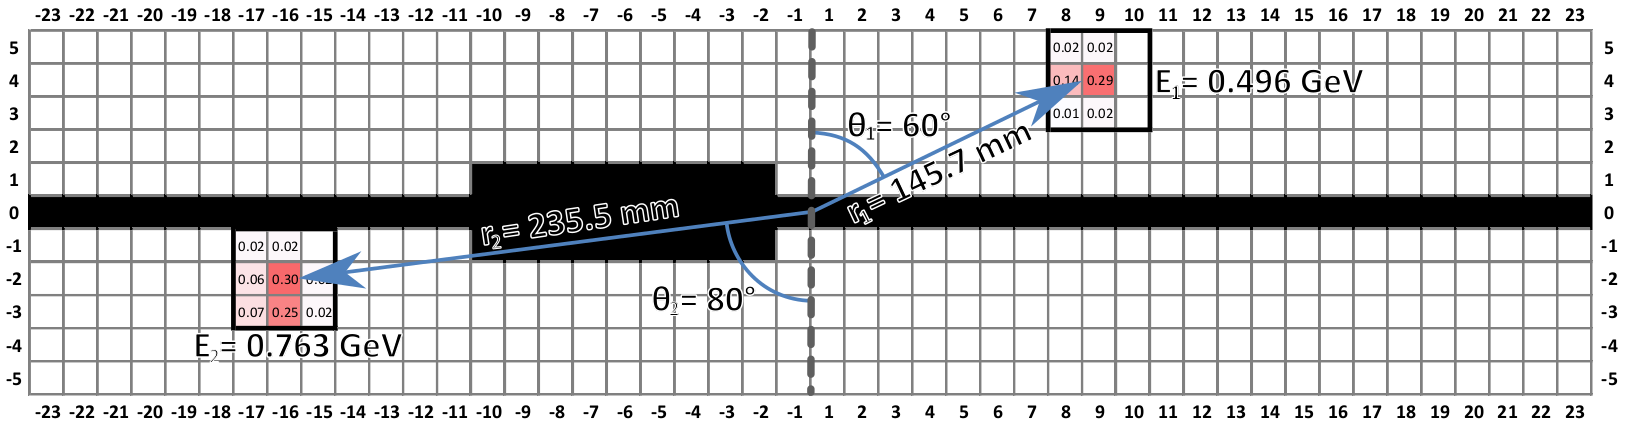
\includegraphics[width=\textwidth]{figures/hps/experiment/smckarty-thesis-fig-27-pair-trigger-depiction.png}
  \caption{
    Figure 27 of \cite{skmccarty-thesis-2020}. Depiction of an event passing the pair trigger
    in the 2016 data collection run. This depiction also displays the variables used in order
    to evaluate events and make the trigger decision.
  }
  \label{fig:hps-pair-trigger-depiction}
\end{figure}
%%%%%%%%%%%%%%%%%%%%%%%%%%%%%%%%%%%%%%%%%%%%%%%%%%%%%%%%%%%%%%%%%%%%%%%%%%%%%%%%
% simulation.tex: Chapter on MC production:
%%%%%%%%%%%%%%%%%%%%%%%%%%%%%%%%%%%%%%%%%%%%%%%%%%%%%%%%%%%%%%%%%%%%%%%%%%%%%%%%
\chapter{Simulation}
\label{chapter:hps:simulation}
%%%%%%%%%%%%%%%%%%%%%%%%%%%%%%%%%%%%%%%%%%%%%%%%%%%%%%%%%%%%%%%%%%%%%%%%%%%%%%%%

Proper study of the iDM signal model necessitates simulating how the HPS detector
would respond if interactions originating from such a process were to occur.

Signal event production flow
\begin{enumerate}
    \item {\sc MadGraph/MadEvent} generation of prompt iDM events
    \item Displacement of decay products in a \emph{uniform} distribution
    \item Simulation of detector response with \textsc{Geant}4 and \texttt{slic}
    \item Emulation of readout
    \item Normal reconstruction pipeline that data retrieved from the detector
          also goes through
\end{enumerate}

Moreover, simulated samples of standard data allows us to study how the detector
responds in the absence of such a signal process. These samples are produced in
a similar way as iDM signal - just with a different original generation step
initializing the event (and inserting the physical displacement distribution
instead of a uniform one).

%%%%%%%%%%%%%%%%%%%%%%%%%%%%%%%%%%%%%%%%%%%%%%%%%%%%%%%%%%%%%%%%%%%%%%%%%%%%%%%%

%%%%%%%%%%%%%%%%%%%%%%%%%%%%%%%%%%%%%%%%%%%%%%%%%%%%%%%%%%%%%%%%%%%%%%%%%%%%%%%%
% reconstruction.tex:
%%%%%%%%%%%%%%%%%%%%%%%%%%%%%%%%%%%%%%%%%%%%%%%%%%%%%%%%%%%%%%%%%%%%%%%%%%%%%%%%
\chapter{Event Reconstruction}
\label{reconstruction_chapter}
%%%%%%%%%%%%%%%%%%%%%%%%%%%%%%%%%%%%%%%%%%%%%%%%%%%%%%%%%%%%%%%%%%%%%%%%%%%%%%%%

%%%%%%%%%%%%%%%%%%%%%%%%%%%%%%%%%%%%%%%%%%%%%%%%%%%%%%%%%%%%%%%%%%%%%%%%%%%%%%%%

\chapter{Data Set}
\label{chapter:hps:dataset}

Proper search for \ac{dm} signals within the \ac{hps} detector includes both collection of data
with the \ac{hps} detector and simulation of how this apparatus responds to the physics of specific
processes. This chapter is focused on detailing the origin of these samples. The collected data can
be characterized by the known inputs from \ac{cebaf} and the run time. The simulation, as one might
expect, is a complicated multi-stage procedure in order to appropriately reflect the intricacies of
the real data.

\section{Collected Data} \label{sec:hps:data}
The data used in this study was collected over a series of 82 data collection runs within 2016
yielding a total of approximately one week of continuous beam.
\todo[detail]{Need to explain luminosity with example from SM, maybe tridents?}
The full luminosity of this data is estimated to be \qty{10.7}{pb^{-1}}.
As alluded to in \cref{sec:hps-ecal}, the collected data was triggered in order to focus the sample on
specific data of interest.

\subsection{Pair 1 Trigger} \label{sec:hps:data:trigger}
The trigger used for this and other physics analyses of the 2016 dataset is the so-called ``Pair 1 Trigger''
designed to select events where evidence for both an electron and positron have been found.
This trigger algorithm combines requirements on the energies of the clusters formed at the trigger
level along with the cluster locations.

After the hits in the \ac{ecal} are clustered, the clusters are selected such that they are of
high enough quality - implemented with energy $E$ and hit multiplicity $N$ cuts.
$$
  E_\mathrm{low} \leq E \leq E_\mathrm{high} \qquad N \geq N_\mathrm{min}
$$
With a beam energy of \qty{2.3}{\GeV}, we set $E_\mathrm{high}=\qty{1.4}{\GeV}$ to help remove
near-full-energy beam electrons from being included within this trigger.
$E_\mathrm{low} = \qty{0.15}{\GeV}$ and $N_\mathrm{min}=2$ are set to these values to suppress
the effect of noise.

All possible pairs of clusters passing these criteria where one of the pair is in the top half of
the \ac{ecal} and the other is in the bottom are then tested with further pair-wise criteria.
Let the top (bottom) cluster have energy $E_\mathrm{top}$ ($E_\mathrm{bot}$) and position
$(x_\mathrm{top},y_\mathrm{top})$ ($(x_\mathrm{bot},y_\mathrm{bot})$) leading to radius
$r_\mathrm{top} = \sqrt{x_\mathrm{top}^2+y_\mathrm{top}^2}$
($r_\mathrm{bot} = \sqrt{x_\mathrm{bot}^2+y_\mathrm{bot}^2}$).

The total energy of both clusters $E_\mathrm{top}+E_\mathrm{bot}$ is bounded below
by $E_\mathrm{sum,low}$ to remove noise and above by $E_\mathrm{sum,high}$ to reduce
the common single-bremsstrahlung background process.
The clusters are required to have an absolute difference $|E_\mathrm{top}-E_\mathrm{bot}| < E_\mathrm{diff}$
to select cluster pairs originating from the same particle.
The energy and position of the lower-energy cluster is required to satisfy
$E + r F \geq E_\mathrm{slope}$ which accounts for the expected bending of
the lower-energy particle's location in the magnetic field (which is failed
by clusters originating from photons which do not bend in the magnetic field).
$F$ is determined from the geometry of the detector and strength of magnetic
field to be $\qty{5.5}{\MeV\mm^{-1}}$.
Finally, the clusters are required to be coplanar within an angle $\phi$ to
again select for clusters originating from the same particle.
$$
  |\tan^{-1}(x_\mathrm{top}/y_\mathrm{top}) - \tan^{-1}(x_\mathrm{bot}/y_\mathrm{bot})| < \phi
$$

These requirements and the values selected for their thresholds are summarized
in \cref{tab:pair-1-trigger}.

\begin{table}[h]
  \centering
  \begin{tabular}{|r|c|c|}
    \hline
    Description & Variable & Value \\ \hline
    Single-Cluster Energy Minimum & $E_\mathrm{low}$ & \qty{0.15}{\GeV} \\
    Single-Cluster Energy Maximum & $E_\mathrm{high}$ & \qty{1.40}{\GeV} \\
    Single-Cluster Hit Count Minimum & $N_\mathrm{min}$ & 2 \\
    \hline
    Cluster Pair Energy Sum Minimum & $E_\mathrm{sum,low}$ & \qty{0.60}{\GeV} \\
    Cluster Pair Energy Sum Maximum & $E_\mathrm{sum,high}$ & \qty{2.00}{\GeV} \\
    Cluster Pair Energy Difference Maximum & $E_\mathrm{diff}$ & \qty{1.14}{\GeV} \\
    Low-Energy Cluster Slope Minimum & $E_\mathrm{slope}$ & \qty{0.70}{\GeV} \\
    Cluster Pair Azimuthal Difference Maximum & $\phi$ & \qty{35}{\degree} \\
    \hline
  \end{tabular}
  \caption{Values for cuts used within the Pair 1 Trigger during data collection of the HPS 2016 dataset.}
  \label{tab:pair-1-trigger}
\end{table}


\section{Simulation} \label{sec:hps:sim}
As mentioned the simulation goes through many steps in order to account for the different physics
processes that are of interest in a realistic fashion. In general, these steps are
\begin{enumerate}
  \item Generation -- using a tool like \textsc{MadGraph/MadEvent}\cite{madgraph4-2007,madgraph5-2014}
        to generate specific events from Feynman diagrams
  \item Displacement -- if the sample expects to have the decay products be displaced (for example in the
        SIMP signal process), displace these decay products with a \emph{uniform} distribution of decay
        lengths to allow for re-weighting.
  \item Simulation -- simulate the detector response with \textsc{Geant4}\cite{geant4}
  \item Emulation -- emulate the readout electronics and triggering mechanism of collected data
\end{enumerate}
After this emulation stage, we can treat the simulation the same as the collected data,
applying the reconstruction and further analysis manipulatiuons and selections.

Both simulated samples of standard processes as well as hypothetical signal processes proceed this way
just with a different original generation step initializing the event. For standard processes, we also
use a physical displacement distribution as understood from prior measurements rather than a uniform
one that is more helpful for reweighting later in analysis.

\section{Reconstruction}
The two subsystems are first reconstructed separately.
The \ac{ecal} produces clusters of nearby hits whose energy
have been corrected by more refined calibration tables.
The \ac{svt} produces tracks using \ac{kf} to find tracks
and \ac{gbl} to fit these tracks to the detector model including
the possibility of in-detector small scatters.
Tracks are then paired with clusters whose position and energy
are close to what the track's position and energy would be at
the \ac{ecal} - such pairs are referred to as reconstructed
particles.
Pairs of reconstructed particles are then used to deduce a
vertex by determing a best-fit location for where the two tracks
intersect one another.
The particle pairs used within this analysis are required to reside
within opposite volumes (i.e. one particle has a track (cluster)
in the top half of the \ac{svt} (\ac{ecal}) and the other has its
constituents in the bottom half); however, vertices from pairs
without this requirement are reconstructed and available for
other analyses.

\section{Analysis Pre-Selection}
The final stage that all events go through is a rudimentary pre-selection which chooses events
that are of higher quality and conform to our expectation of signal topology and simplifies the
resulting shape of the data in the event such that final analysis is not as complicated.
Specifically, the pre-selection for this analysis is requiring exactly one quality vertex to be
reconstructed within the event.
This requirement naturally disposes of events which are cluttered with particles from other beam arrivals
(thus causing more than one vertex to be reconstructed) and
events which do not have a electron-positron pair within acceptance (thus causing no vertices to be
reconstructed).
The requirements for a ``quality'' vertex were developed and optimized by 
prior work\cite{aspellman-thesis-2024} and are standardized within \ac{hps} analyses.
\cref{fig:vertex-pre-selection} shows the relative efficiency of these requirements.
\cref{fig:n-vertex-pre-selection} shows the distribution of number of vertices
that pass these criteria.
\cref{fig:event-pre-selection} shows the summary of this pre-selection requirement including the relative
efficiency of the quality vertex requirements.

The largest drop in signal efficiency is from the requirement that a quality vertex is found
within the event.
With the relatively high efficiency of the vertex pre-selections, this drop in efficiency
can be interpreted as mainly due to the geometric acceptance of the \ac{hps} detector.
Fortunately, the background processes are removed in higher proportion from this requirement.

\begin{figure}
  \centering
  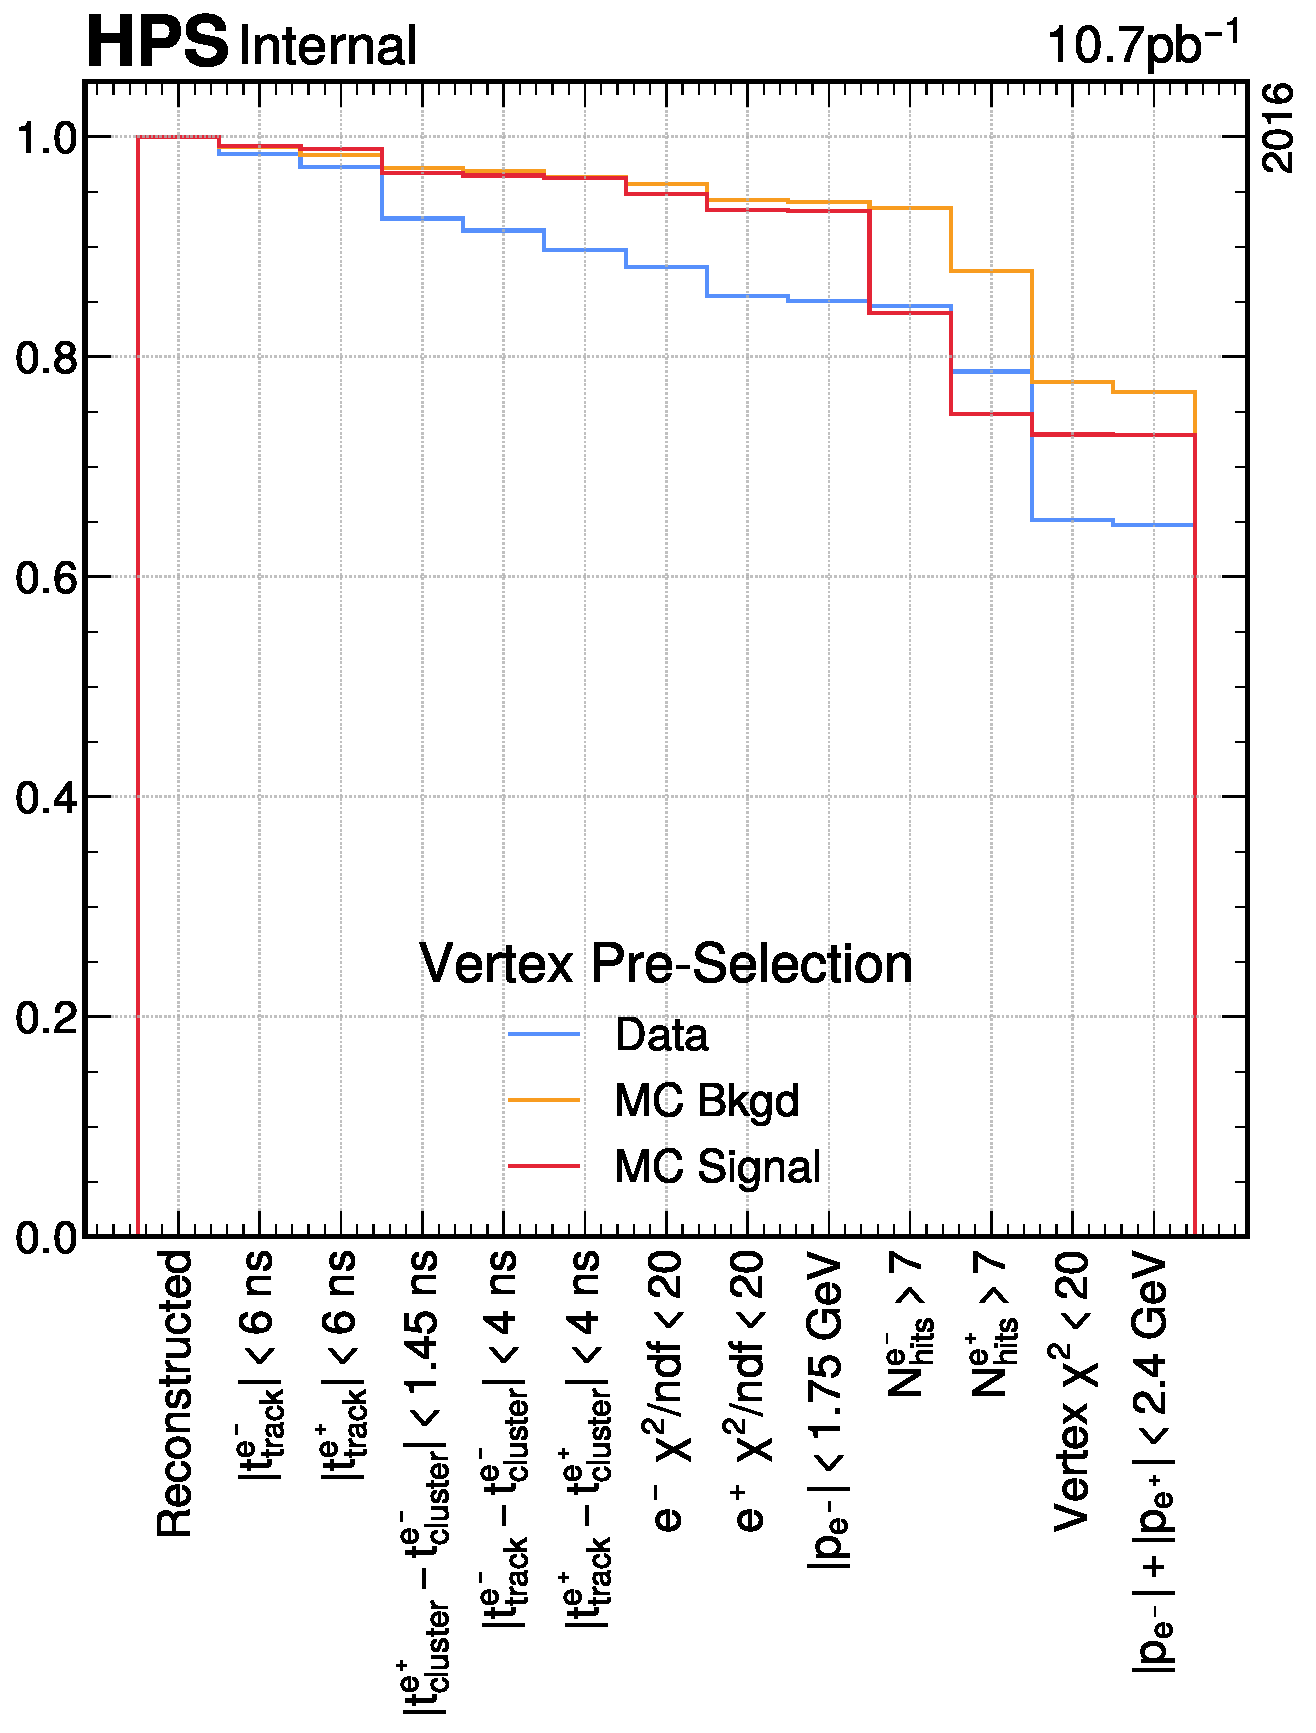
\includegraphics[width=0.5\textwidth]{figures/hps/dataset/vertex-pre-selection-efficiency.pdf}
  \caption{Relative efficiency of vertex quality pre-selection requirements.}
  \label{fig:vertex-pre-selection}
\end{figure}

\begin{figure}
  \centering
  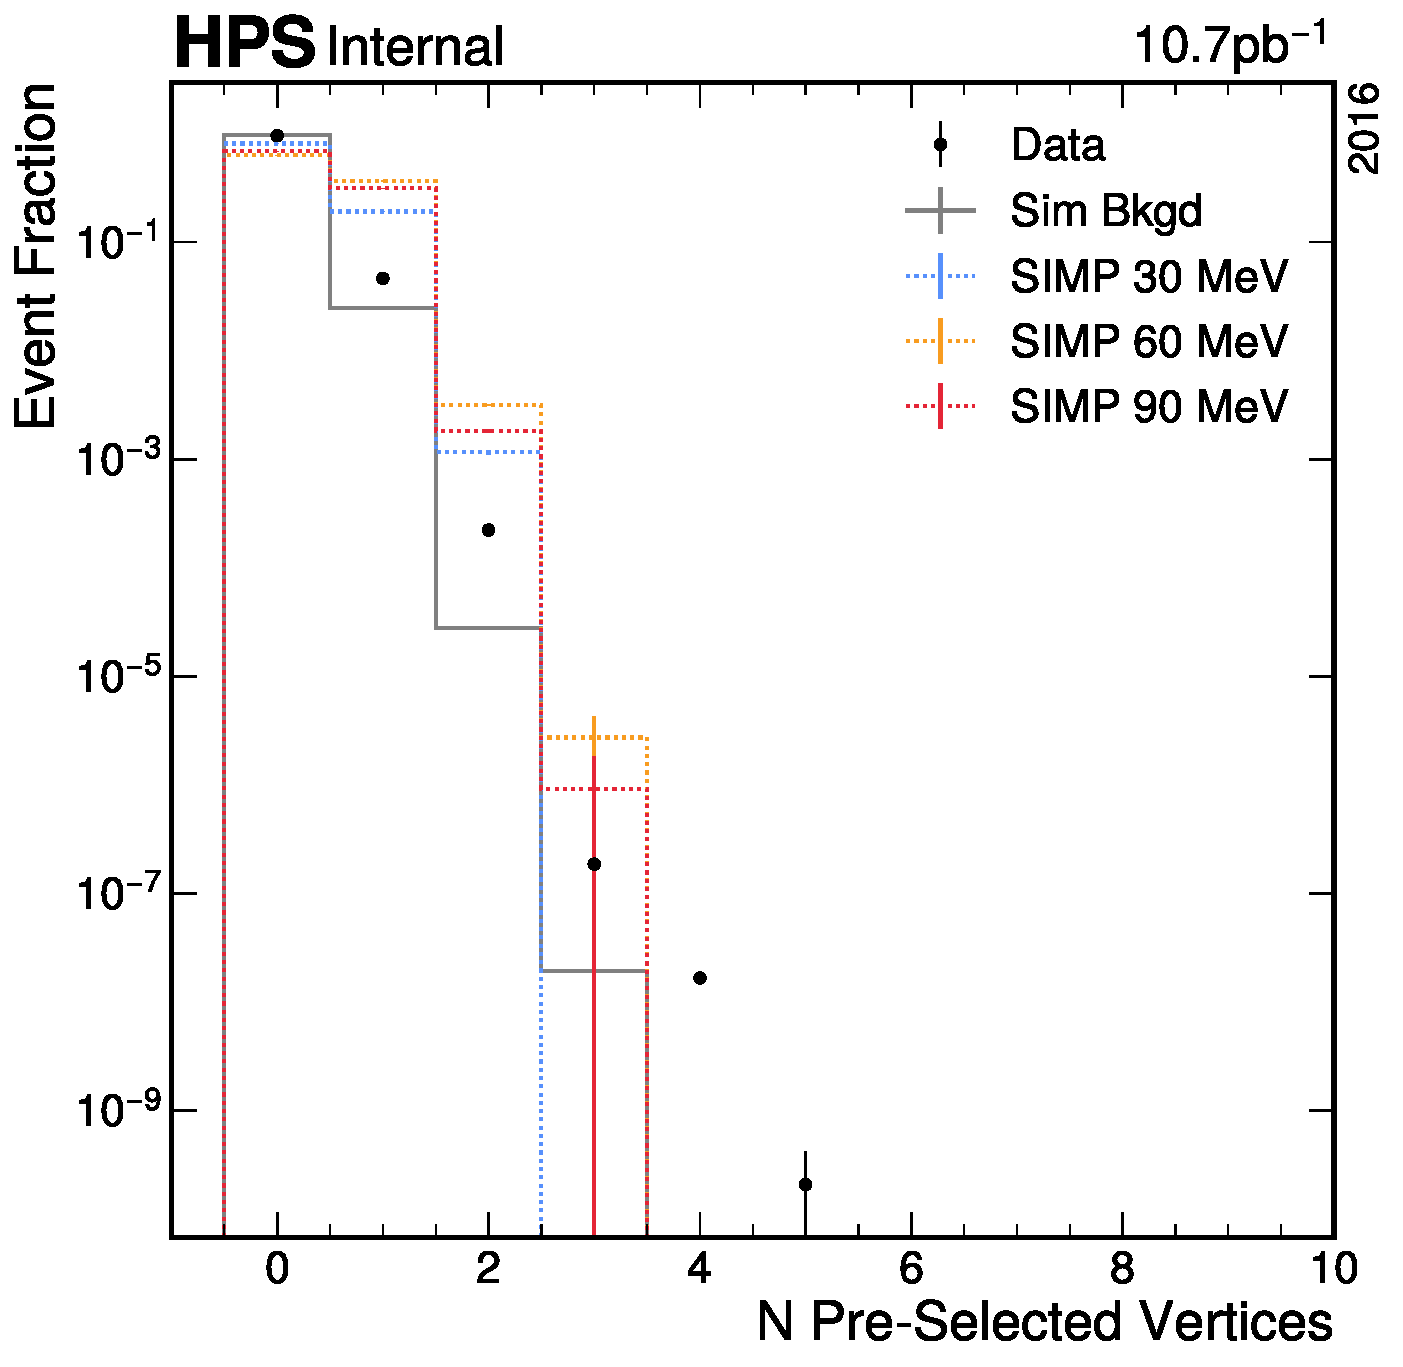
\includegraphics[width=0.5\textwidth]{figures/hps/dataset/n-pre-selected-vertices.pdf}
  \caption{Number of vertices passing the quality pre-selection.}
  \label{fig:n-vertex-pre-selection}
\end{figure}

\begin{figure}
  \centering
  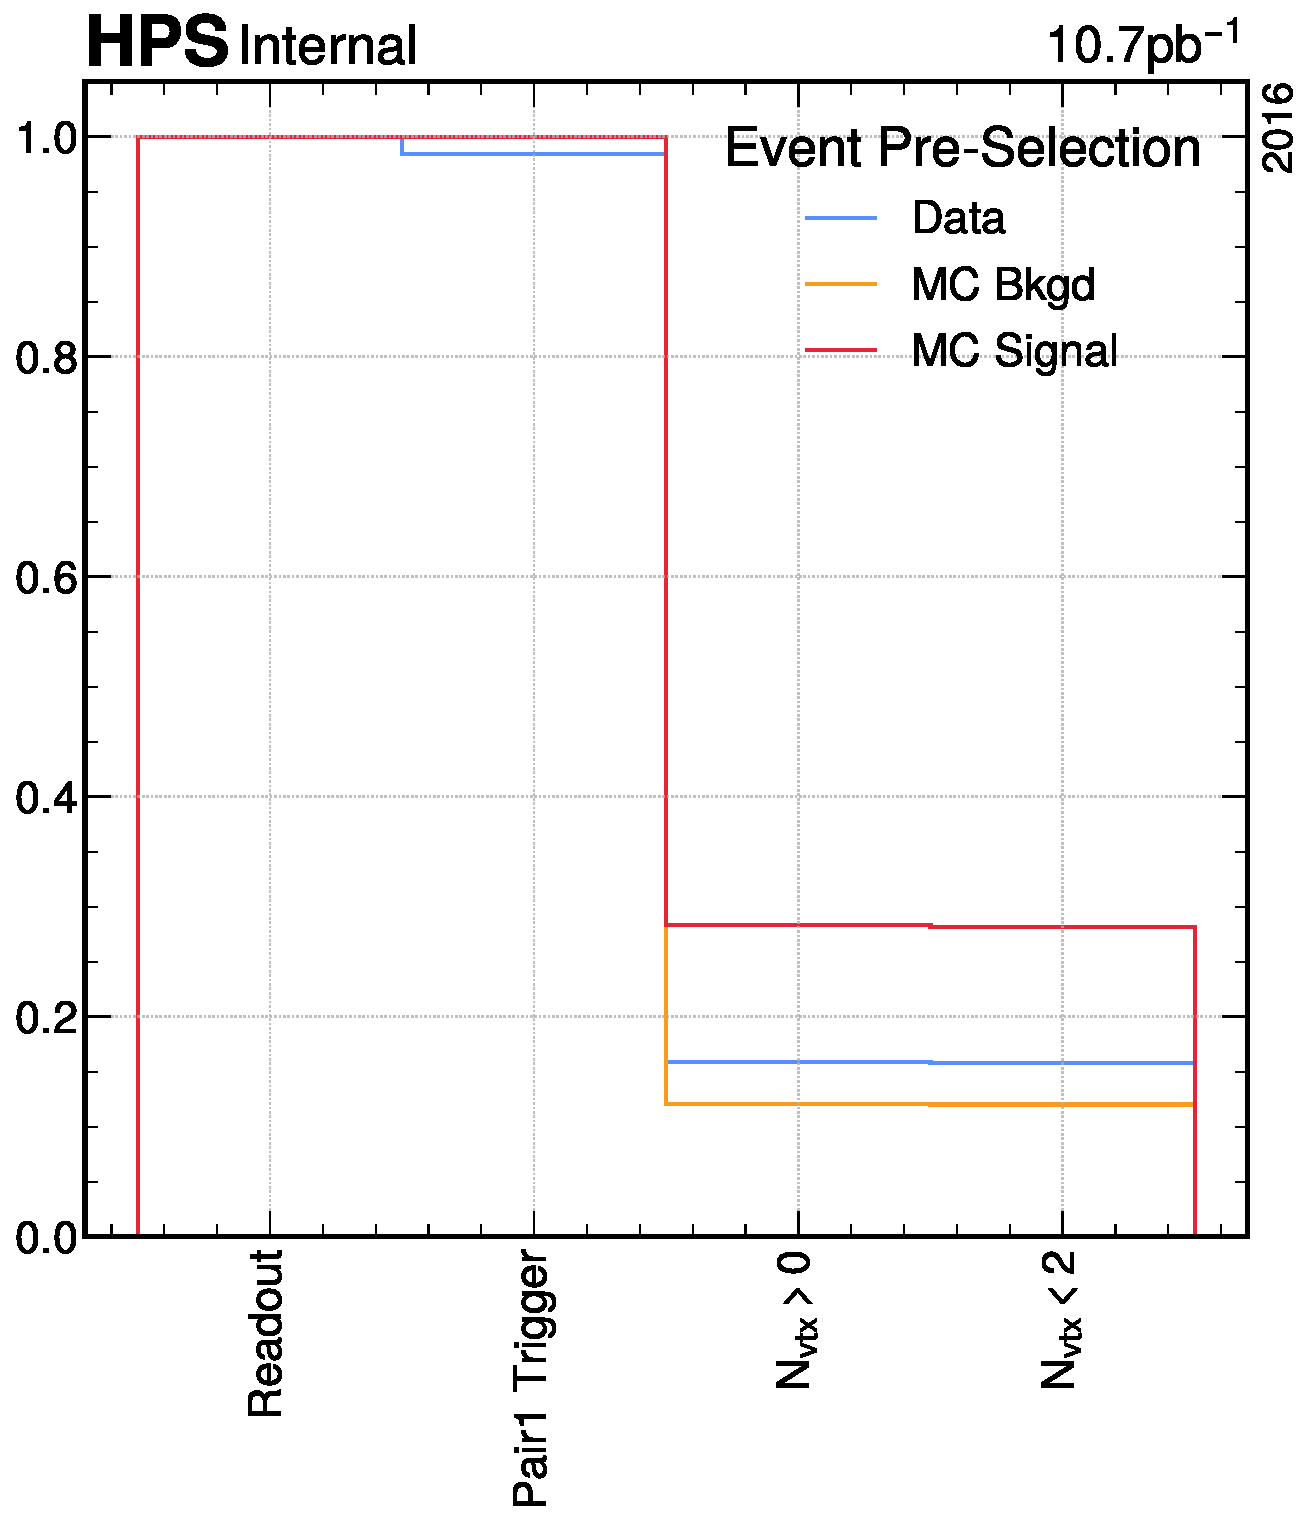
\includegraphics[width=0.5\textwidth]{figures/hps/dataset/event-pre-selection-efficiency.pdf}
  \caption{Relative efficiency of pre-selection of events.
  $N_\mathrm{vtx}$ is the number of vertices passing the vertex pre-selection requirements.
  Since other triggers for different purposes are present in the data, the Pair 1 Trigger
  is applied to data but not to simulation.}
  \label{fig:event-pre-selection}
\end{figure}


%%%%%%%%%%%%%%%%%%%%%%%%%%%%%%%%%%%%%%%%%%%%%%%%%%%%%%%%%%%%%%%%%%%%%%%%%%%%%%%%
% event_selection.tex: Select of showering and tracking events:
%%%%%%%%%%%%%%%%%%%%%%%%%%%%%%%%%%%%%%%%%%%%%%%%%%%%%%%%%%%%%%%%%%%%%%%%%%%%%%%%
\chapter{Event Selection}
\label{chapter:hps:selection}
%%%%%%%%%%%%%%%%%%%%%%%%%%%%%%%%%%%%%%%%%%%%%%%%%%%%%%%%%%%%%%%%%%%%%%%%%%%%%%%%

%%%%%%%%%%%%%%%%%%%%%%%%%%%%%%%%%%%%%%%%%%%%%%%%%%%%%%%%%%%%%%%%%%%%%%%%%%%%%%%%

\chapter{Analysis}
\label{chapter:hps:analysis}

A search for visibly-decaying \ac{dm} is not novel, many experiments have been purposed
built for such a search; however, \ac{hps} is specially focused on \ac{dm} that decays
within shorter distances.
While \ac{hps} has previously searched \cite{hps-2016-displaced-vtx} for simple dark sectors
more similar to the benchmark model used within the \ac{ldmx} missing energy search,
no \ac{dm} was found and the longer decay lengths of this dark sector model greatly
impacted the resulting sensitivity of \ac{hps}.
\cref{sec:hps:simps} introduced the idea of \ac{simp} \ac{dm} which has additional
interest for \ac{hps}.
Specifically, the increase in complexity of the \ac{dm} model slightly decouples the production
rate from the decay rate meaning the number of events were \ac{dm} is produced is not as tightly
connected to how displaced the particles are expected to be within the detector.
The downside of this decoupling is that some energy is lost to the production of the lighter
dark meson $\pi_D$ when the dark photon decays within the dark sector; however,
this also means \ac{hps} has not searched this regime since one of the key selections within
its previous displaced vertex search was requiring the total momentum of the vertex to
near the beam energy instead of significantly below it.

With the samples presented in \cref{chapter:hps:dataset}, a search for \acp{simp} within the collected
data has been performed.
An additional, orthogonal category of data was introduced to be combined with prior work,
enabling higher sensitivity to a range of \ac{simp} parameter space.

\section{Signal Yield}

The expected signal yield is a crucial part of any kind of search analysis
and this one is no exception.
The prior search within \ac{ldmx} benefited from its missing momentum/energy technique
in this regard since the mixing strength $\epsilon$ is only connected to the scale of the signal
yield and not how the signal events would present themselvs in the data.
In a visible search, the mixing strength also effects the decay length and thus a more intricate
signal yield estimate is required to account for the fact that changing $\epsilon$ not only changes
the magnitude but also changes which events are more likely to be observed within data.

In this analysis, we modify the expected signal yield calculation done previously by \ac{hps}
in \cite{hps-2016-displaced-vtx} to accomodate the two viable decay channels within this \ac{simp} model.
Nevertheless, the full signal yield calculation is summarized here for reference.

The magnitude of this estimate is set by the relationship between dark photon production cross section
and the radiative trident differential cross section\cite{bjorken-ap-rate:2009}.
\begin{equation}
  \sigma_{A'} = \epsilon^2\frac{3\pi}{2\alpha} m_{A'} \left.\frac{d\sigma_{\gamma^*}}{dm}\right|_{m=m_{A'}}
\end{equation}
Multiplying both sides by the dataset's luminosity then gives us event yields.
\begin{equation}
  N_{A'} = \epsilon^2\frac{3\pi}{2\alpha} m_{A'} \left.\frac{dN_{\gamma^*}}{dm}\right|_{m=m_{A'}}
\end{equation}
The complexity arises when we remember that specifically radiative tridents are not
directly observable -- they are intertwined with other standard processes that produce
the same outgoing particles (Bethe-Heitler tridents for example).
Thus, we estimate the radiative trident differential yield $dN_{\gamma^*}/dm$ by
modifying the observable trident differential yield $dN_{3e\mathrm{,CR}}/dm_\mathrm{reco}$ by
two simulation-derived factors.
The radiative fraction $f_\mathrm{rad}$ estimates the fraction of trident events
that originate from the radiative process.
\begin{equation}
  f_\mathrm{rad} = \frac{dN_{\gamma^*}}{dm} \bigg/ \frac{dN_{3e}}{dm_\mathrm{reco}}
\end{equation}
And the radiative acceptance times efficiency $A_\mathrm{rad}$ estimates the
fraction of trident events that are within the geometric acceptance of the detector
and pass the trigger and preselection requirements.
\begin{equation}
  A_\mathrm{rad} = \frac{dN_{3e,CR}}{dm_\mathrm{reco}} \bigg/ \frac{dN_{3e,\mathrm{gen}}}{dm_\mathrm{reco}}
\end{equation}
where CR stands for the Control Region in \Psum
(see \cref{sec:hps:analysis:variables} for the definition of this variable).
Thus, the expected yield of dark photons created within the detector
but not necessarily within its acceptance or passing selection requirements is
\begin{equation}
  N_{A'} = \epsilon^2\frac{3\pi}{2\alpha} m_{A'} 
    \frac{f_\mathrm{rad}}{A_\mathrm{rad}}
    \left.\frac{dN_{3e\mathrm{,CR}}}{dm_\mathrm{reco}}\right|_{m=m_{A'}}
\end{equation}
Both $f_\mathrm{rad}$ and $A_\mathrm{rad}$ use the event and vertex pre-selection before
any downstream analysis selections.
They parameters for these polynomials are given in \cref{tab:rad-poly-coeff}
and these ingredients along with the resulting $N_{A'}$ is given in \cref{fig:dark-photon-yield-calc}.

\begin{table}
  \centering
  \begin{tabular}{c|cc}
    Coefficient     & $f_\mathrm{rad}$ & $A_\mathrm{rad}$ \\ \hline
    $c_0$           & 0.10541434 & -0.48922505 \\
    $c_1$ / MeV     & -0.0011737697 & 0.073733061 \\
    $c_2$ / MeV$^2$ & \num{7.4487930e-06} & \num{-0.0043873158} \\
    $c_3$ / MeV$^3$ & \num{-1.6766332e-08} & 0.00013455495 \\
    $c_4$ / MeV$^4$ & 0.0 & \num{-2.3630535e-06} \\
    $c_5$ / MeV$^5$ & 0.0 & \num{2.5402516e-08} \\
    $c_6$ / MeV$^6$ & 0.0 & \num{-1.7090900e-10} \\
    $c_7$ / MeV$^7$ & 0.0 & \num{7.0355585e-13} \\
    $c_8$ / MeV$^8$ & 0.0 & \num{-1.6215982e-15} \\
    $c_9$ / MeV$^9$ & 0.0 & \num{1.6032317e-18} \\
  \end{tabular}
  \caption{%
    Polynomial coefficients for radiative fraction and acceptance functions.
    All decimal points are given for reproducibility; however, not all
    of them are significant.
  }
  \label{tab:rad-poly-coeff}
\end{table}

\begin{figure}
  \centering
  \begin{subfigure}[T]{0.48\textwidth}
    \centering
    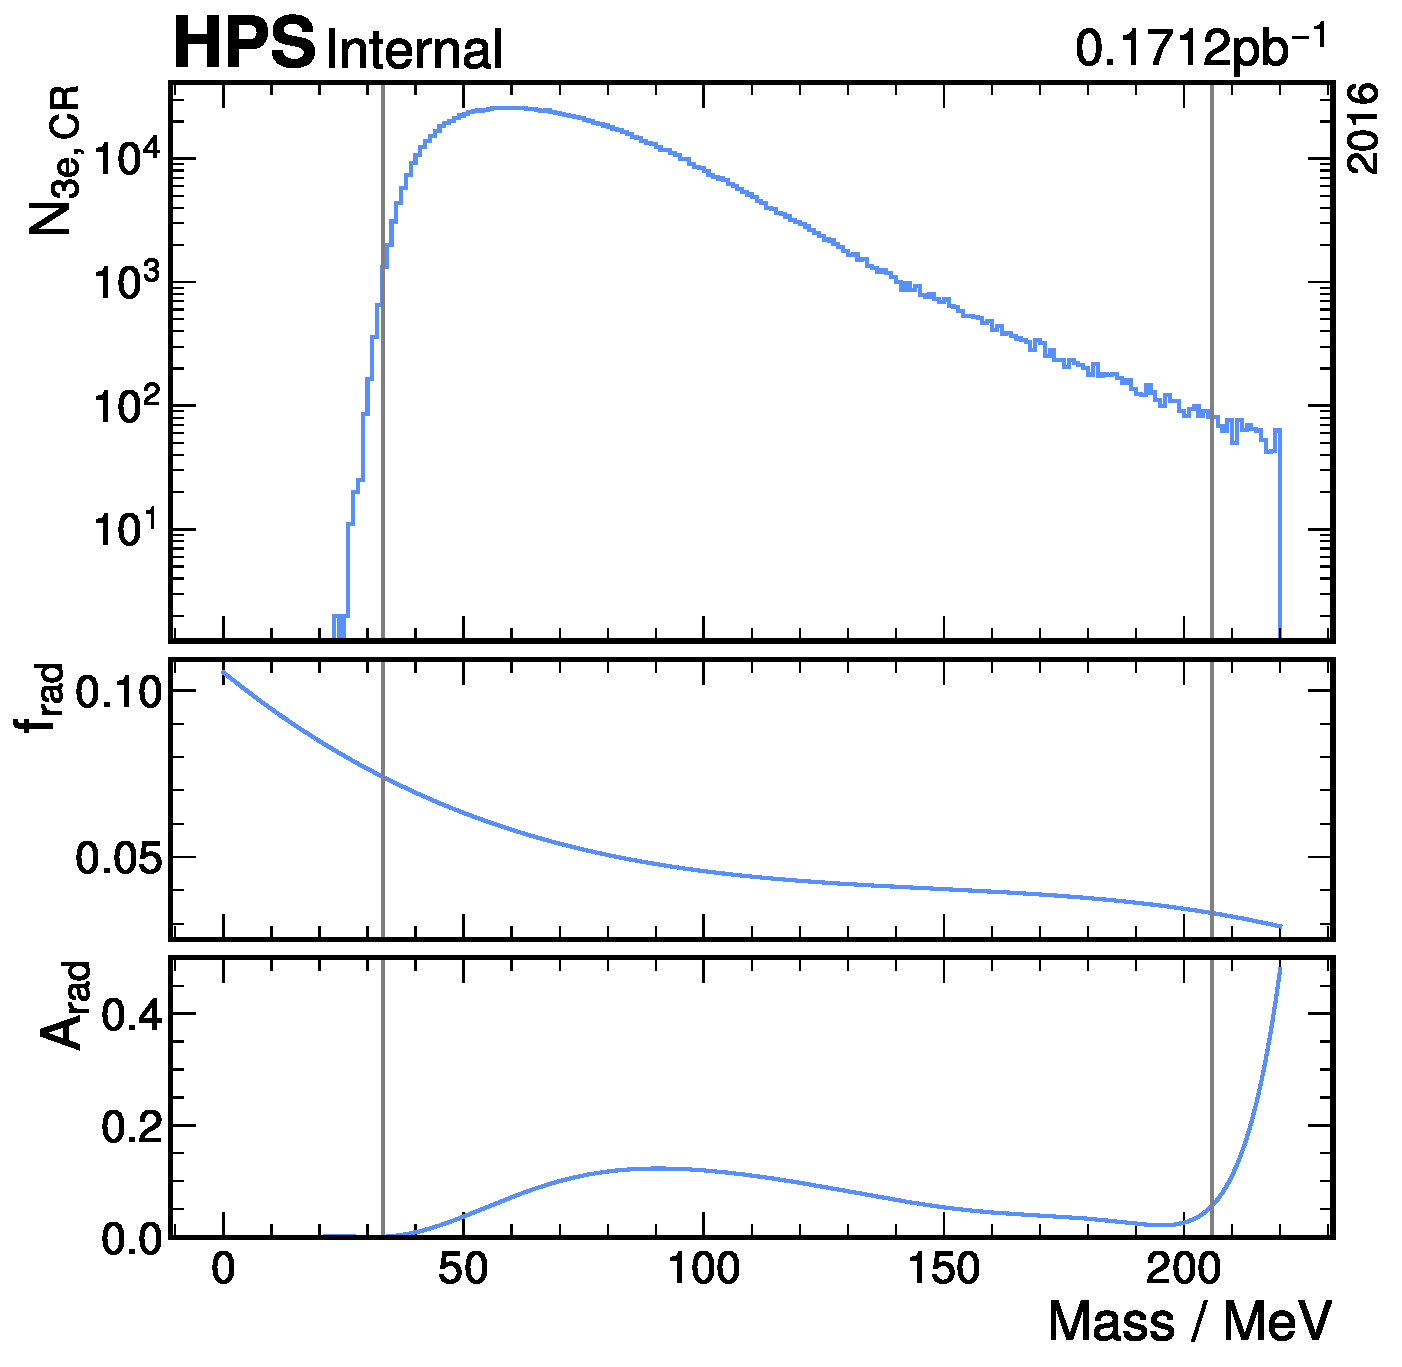
\includegraphics[width=\textwidth]{figures/hps/analysis/signal-yield/dark-photon-yield-calc-ingredients.pdf}
    \caption{Ingredients to the total dark photon yield calculation including
    the observed trident yield (top), radiative fraction (middle), and
    radiative acceptance (bottom).}
    \label{fig:dark-photon-yield-calc:ingredients}
  \end{subfigure}
  \begin{subfigure}[T]{0.48\textwidth}
    \centering
    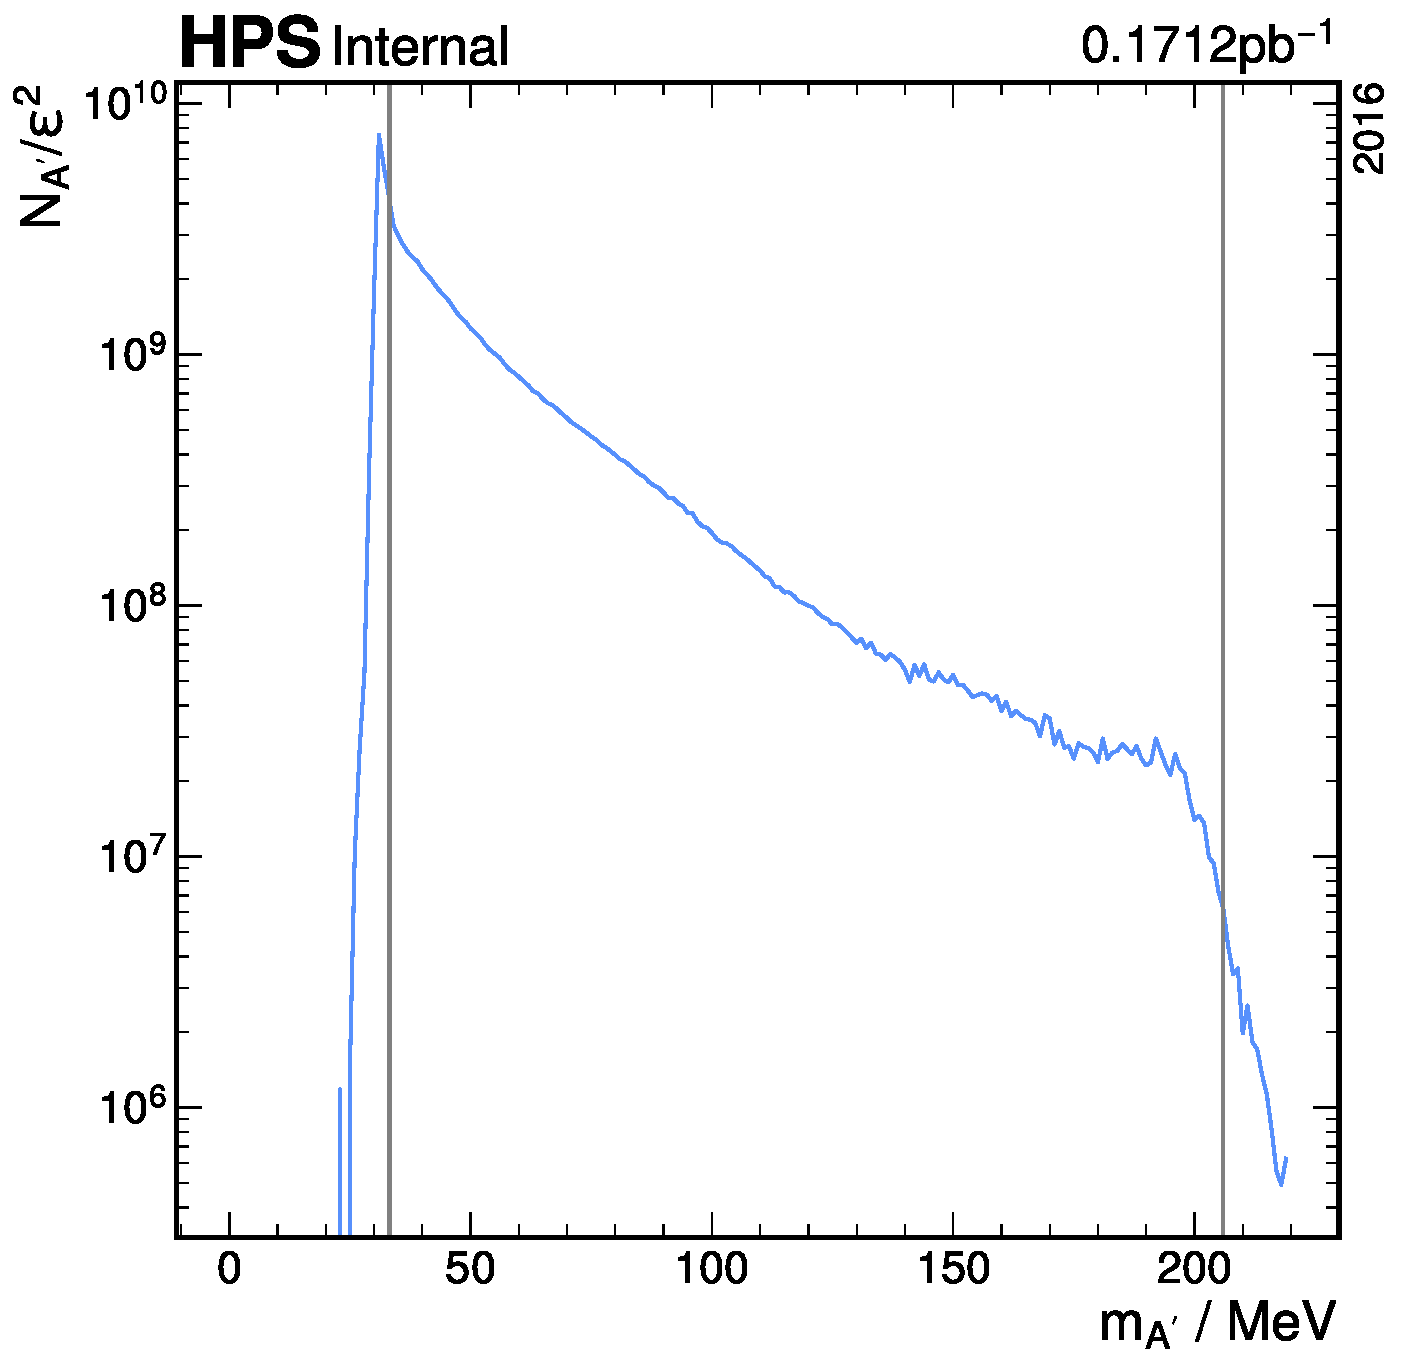
\includegraphics[width=\textwidth]{figures/hps/analysis/signal-yield/dark-photon-yield-calc-result.pdf}
    \caption{Resulting total dark photon yield.}
    \label{fig:dark-photon-yield-calc:result}
  \end{subfigure}
  \caption{Depiction of dark photon yield calculation using a single run
  of the data ($\sim\qty{1.6}{\%}$).
  The gray vertical lines show the bounds of the search using the
  nominal ratio $m_{A'}/m_{V_D} = 1.66$.}
  \label{fig:dark-photon-yield-calc}
\end{figure}

In this signal hypothesis, we do not observe the dark photon's production or decay,
instead, the dark photon decays to an unobservable dark pion and the neutral dark
vector meson $V_D$ which in turn is what decays back into a standard model electron-positron pair.
The above calculation of $N_{A'}$ accounts for the dark photon's production, but
we need to account for the dark photon's decay and the dark vector meson's decay.
The first decay has a branching ratio $BR(A'\to\pi_D V_D)$ which is complicated
by the fact that there are actually two different dark neutral vector mesons that
fit our requirements.
The second process is embedded in the decay rate of the dark vector meson to
electron-positron pairs $\Gamma(V_D\to e^+e^-)$.\footnote{
  There are other decay processes of the $V_D$!
  Namely, the so-called ``three-prong'' decay $V_D\to\pi_De^+e^-$ would
  greatly increase the potential rate at the cost of preventing the $e^+e^-$
  from reconstructing the $m_{V_D}$ mass resonance.
}
Let $E(z)$ be the signal efficiency of the analysis as a function of the $z$ where the
$V_D$ decayed into the electron-positron pair.
Then we can sum over the possible $V_D$ and estimate the fraction of $N_{A'}$
that produce a $V_D$ which decays and passes the analysis requirements.
\begin{equation}
  N_\mathrm{sig} = N_{A'}\int_{z_\mathrm{target}}^\infty \sum_{V_D} D_{V_D}(z)E(z) dz
\end{equation}
where
\begin{equation}
  D_{V_D}(z) = BR(A'\to\pi_D V_D)
  \frac{e^{-(z-z_\mathrm{target})/(\gamma c \tau_{V_D})}}{\gamma c \tau_{V_D}}
\end{equation}
The branching ratio $BR(A'\to\pi_D V_D)$ and lifetime $\tau_{V_D}$ are taken
from \cite{simp-pheno-2018} (along with the general procedure of this estimate).
What is important to remember is that the lifetime is dependent on $\epsilon^2$,
so while increasing $\epsilon^2$ increases $N_{A'}$ it also makes the lifetime shorter
and thus the $V_D$ decay ``looks'' more like standard un-displaced background.

The $V_D$ energy (and thus the relativisitic $\gamma$) used in $D_{V_D}(z)$
is only distributed over a small range (within $\mathcal{O}(\qty{100}{\MeV})$)
so we replace it with the mean $\langle\gamma\rangle$ in order to make the
calculation more practical.
Additionally, we impose an upper limit on the decay $z$ to be \qty{25}{\cm} after
the target since the efficiency of the reconstruction past $\sim\qty{20}{\cm}$ drops to zero.
\begin{equation}
  N_\mathrm{sig} = N_{A'}
    \int_{0}^{\qty{25}{\cm}} dz'
    \sum_{V_D} \mathrm{BR}(A'\to\pi_D V_D)
    \frac{e^{-z'/(\langle\gamma\rangle c \tau_{V_D})}}{\langle\gamma\rangle c \tau_{V_D}}
    E(z'+z_\mathrm{target})
\end{equation}
where $z' = z-z_\mathrm{target}$.
\cref{fig:n-sig-eg:uniform} shows $N_\mathrm{sig}$ with a uniformly perfect signal efficiency
$E(z) = 1$ to give a sense of scale, but a slightly more realistic example is using a
step-wise signal efficiency $E(z) = 0.1$ if $\qty{20}{\mm} < z < \qty{100}{\mm}$ and $0$ otherwise
\cref{fig:n-sig-eg:step}.

\begin{figure}
  \centering
  \begin{subfigure}{0.48\textwidth}
    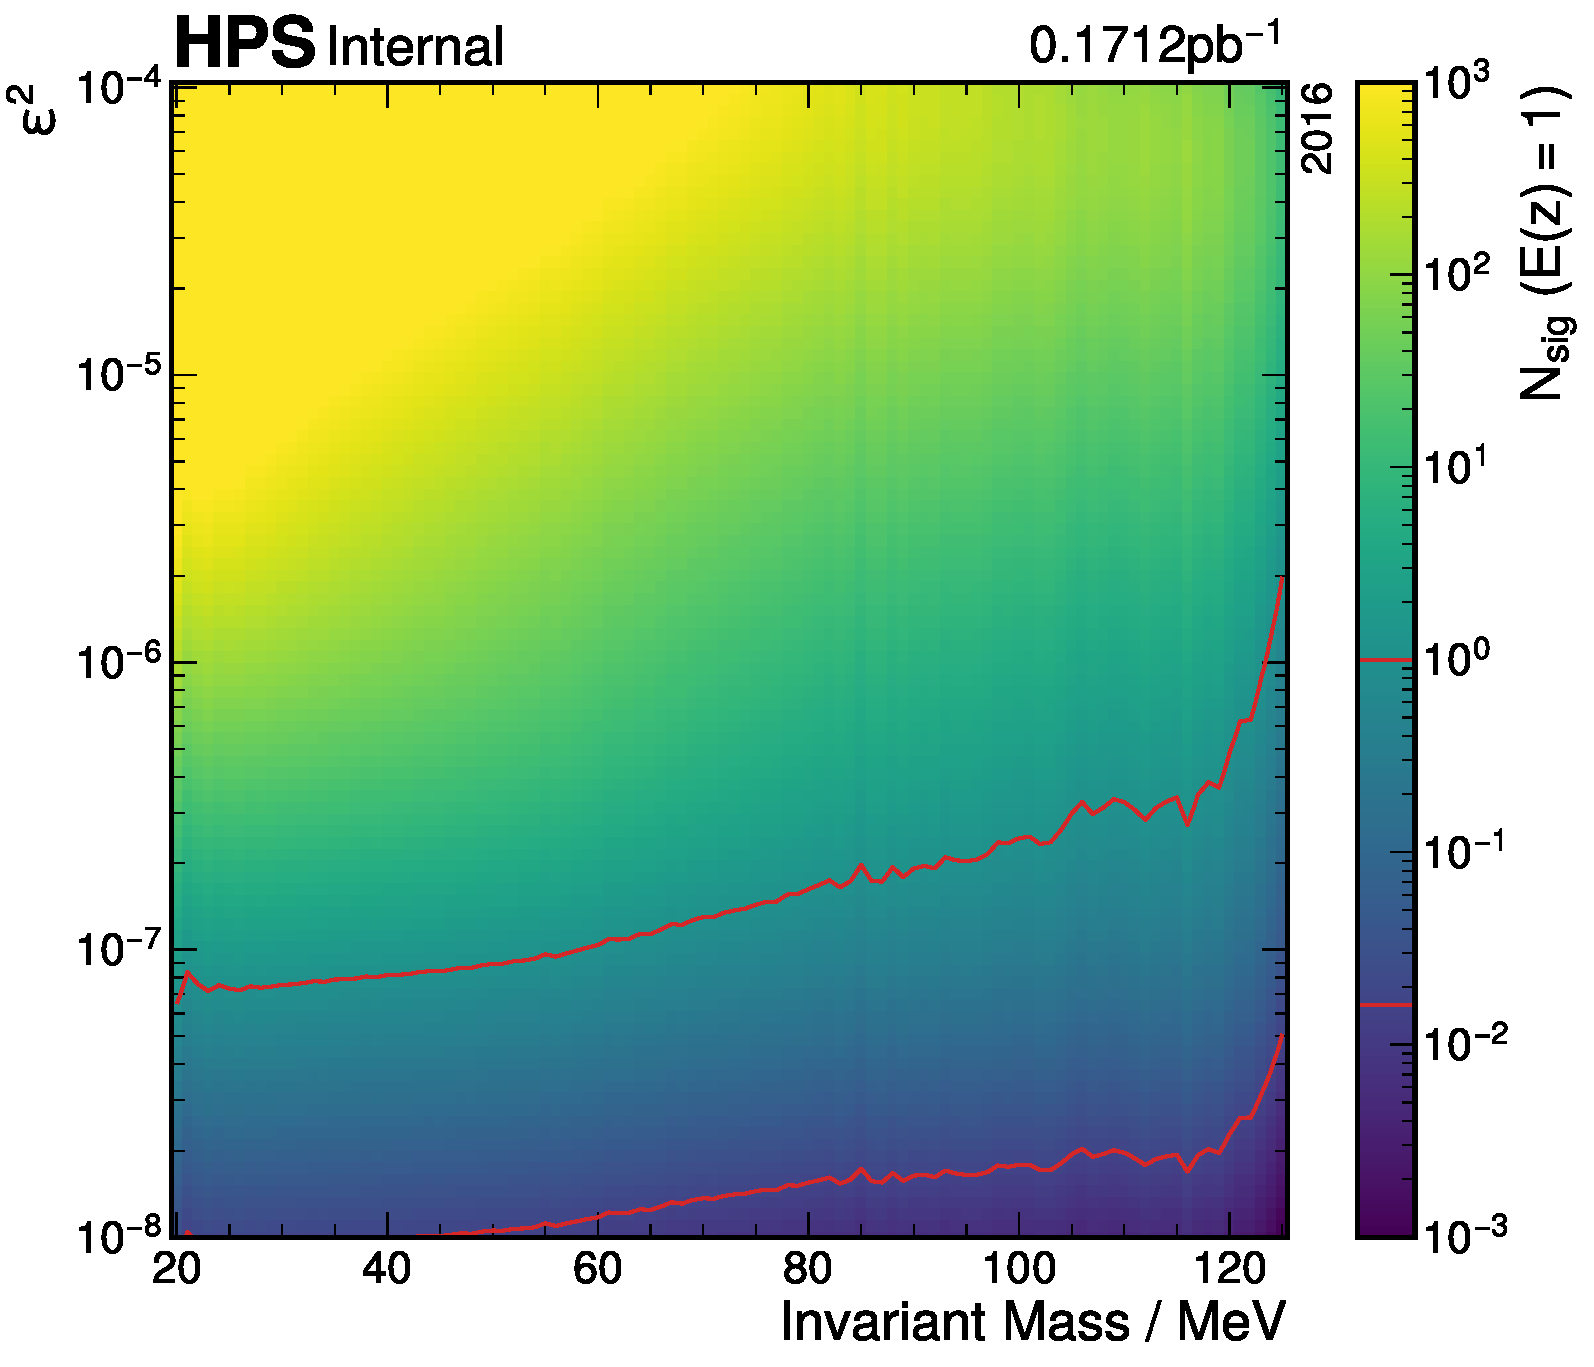
\includegraphics[width=\textwidth]{figures/hps/analysis/signal-yield/n-sig-uniform-eff-1.0.pdf}
    \caption{Uniformly perfect signal efficiency with yield dominated by prompt decays.}
    \label{fig:n-sig-eg:uniform}
  \end{subfigure}
  ~
  \begin{subfigure}{0.48\textwidth}
    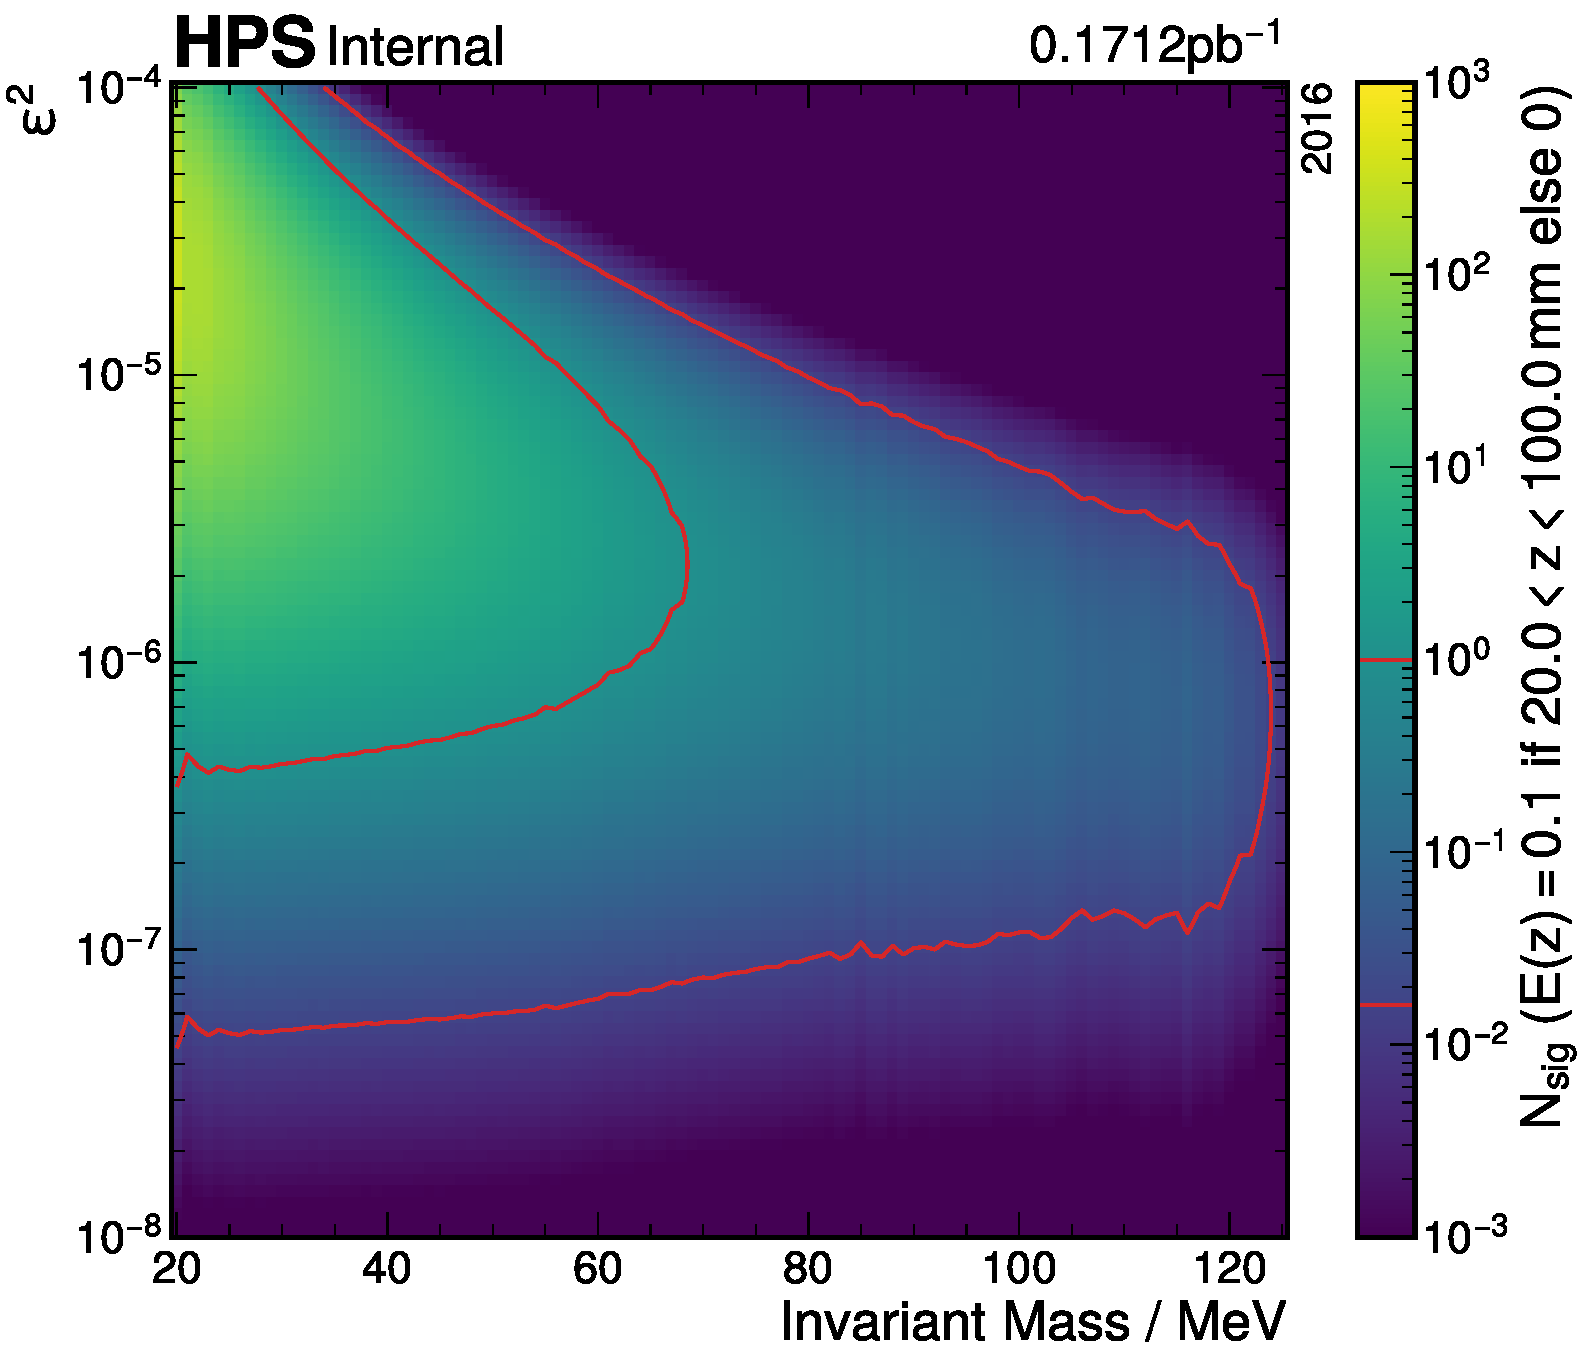
\includegraphics[width=\textwidth]{figures/hps/analysis/signal-yield/n-sig-step-eff-0.1-after-20.0.pdf}
    \caption{A step signal efficiency mocking a perfect analysis cut in displaced vertex $z$.}
    \label{fig:n-sig-eg:step}
  \end{subfigure}
  \caption{Expected signal yield $N_\mathrm{sig}$ for some rudimentary example efficiencies.
  Red contour lines are given at 1 and 1.6\% (the approximate fraction of this data subsample)
  to give a sense of scale.
  Values are ``clipped'' to the color bar (for example, a signal yield of \num{2e4} is colored
  yellow which is marked as \num{1e3}) so we can focus on the important orders of magnitude.}
  \label{fig:n-sig-eg}
\end{figure}

In summary, the key point to make here is that the signal efficiency as a function of true
decay length $E(z)$ is the single analysis-dependent ingredient that effects the resulting
signal yield.
The rest of the ingredients are either fixed by the dataset being searched (e.g. trident
differential production, $f_\mathrm{rad}$, $A_\mathrm{rad}$) or are parameters that we
vary for the search ($\epsilon^2$, $m_{V_D}$).
A moderately realistic signal efficiency shows the range of $\epsilon^2$ and $m_{V_D}$
this dataset has potential sensitivity (\cref{fig:n-sig-eg:step}) which informs the
ranges these values will take below.


\section{Reconstruction Categories}
The design of \ac{hps} separates reconstructed tracks into categories that are
not necessarily associated with the underlying physics for which we are searching.
Specifically, the number of layers (and which layers) that are included within a track
has a large effect on the resulting precision of the reconstructed physics variables
of that track; thus, we categorize vertices on whether one or both of their tracks contain
both sensors in the first layer.
\cref{fig:hps-reco-category-diagram} shows examples of the two categories considered
within this work.
The L1L1 category whose verticies have both tracks with good precision was first studied
for this signal search \todo[citation]{need Alic's thesis} when optimizing the pre-selection
requirements described earlier.

Extending this search to the L1L2 category has a rather simple motivation.
While the vertices may degrade in precision, the additional increase of data both in terms
of total volume and the potential to observe higher-displaced vertices is expected to improve
the sensitivity of the \ac{hps} \ac{simp} search.

\begin{figure}
  \centering
  \begin{subfigure}{0.48\textwidth}
    \centering
    \resizebox{\textwidth}{!}{\begin{tikzpicture}
  \drawhpsfirsttwolayers
  \node at (\targetx,+2) {L1L1};
  \node at (\targetx+1,0.1) [circle,fill,inner sep=1.5pt] {};
  \draw[black,->] (\targetx+1,0.1) -- (2.5,2) node[anchor=north west] {\(e^-\)};
  \draw[black,->] (\targetx+1,0.1) -- (2.5,-1.9) node[anchor=south west] {\(e^+\)};
\end{tikzpicture}
}
  \end{subfigure}
  ~
  \begin{subfigure}{0.48\textwidth}
    \centering
    \resizebox{\textwidth}{!}{\begin{tikzpicture}
  \drawhpsfirsttwolayers
  \node at (\targetx,+2) {L1L2};
  \node at (\targetx+2.0,0.1) [circle,fill,inner sep=1.5pt] {};
  \draw[black,->] (\targetx+2.0,0.1) -- (2.5,2) node[anchor=north west] {\(e^-\)};
  \draw[black,->] (\targetx+2.0,0.1) -- (2.5,-1.8) node[anchor=south west] {\(e^+\)};
\end{tikzpicture}
}
  \end{subfigure}
  \caption{Diagrams showing L1L1 (left) and L1L2 (right) vertex examples.}
  \label{fig:hps-reco-category-diagram}
\end{figure}

\section{Physics Variables}
\label{sec:hps:analysis:variables}
There are many possible variables that could be used to separate candidate signal
vertices from the standard process backgrounds.
While this section is not an exhaustive list of all possible variables,
it does explain the ones used within this analysis as well as motivation for
their use.

The \ac{simp} signal vertex will have significantly less energy than the amount
delivered by the beam because of the production of a light dark meson when the heavier
vector meson $V_D$ is produced.
Thus, a selection on the sum of the momentum magnitudes is applied.
\begin{equation}
  P_\mathrm{sum} = |\vec{p}_{e^-}|+|\vec{p}_{e^+}|
\end{equation}
Specifically, the Signal Region (SR) used for the actual search requires
$\qty{1.0}{\GeV} < $\Psum$ < \qty{1.9}{\GeV}$ and the Control Region (CR)
used for determining the trident differential production rate is
$\qty{1.9}{\GeV} < $\Psum$ < \qty{2.4}{\GeV}$.

Since we are searching for the dark vector boson $V_D$ via its
2-body decay into an electron and a positron, we expect the invariant mass of the vertex $m_\text{reco}$
to be within the resolution of the detector $\sigma_m$ of the mass we are searching for $m_{V_D}$.
\begin{equation}
  p_m = \frac{|m_\text{reco}-m_{V_D}|}{\sigma_m}
\end{equation}
Applying an upper limit on $p_m$ is often refered to as a ``mass window''
since it results in $m_\text{reco}$ residing within a small range around $m_{V_D}$.

Each vertex can be projected back to the target using its position and total momentum,
and the location of the vertex at the target can be compared to the beam
position extracted from a sub-sample of the data\todo[citation]{reference how beamspot extraction is done}.
The separation between the projected position $\vec{x} = (x,y)$ and the beam position
$\vec{\mu} = (\mu_{x'}, \mu_{y'})$ is then measured
and normalized by the width of the beam in that direction $(\sigma_{x'},\sigma_{y'})$.
The distribution of the beamspot is allowed to be rotated relative to our
chosen axes by the angle $\theta_\mathrm{beam}$, meaning we need to rotate $\vec{x}$
before comparing it to the beam spot.
The total ``elliptical'' separation between the reconstructed vertex
projected back to the target and the beam spot can be quantified by
\begin{equation}
  N_\sigma = \sqrt{
    \left(
      \frac{x\cos\theta_\mathrm{beam} - y\sin\theta_\mathrm{beam} - \mu_{x'}}{\sigma_{x'}}
    \right)^2
    +\left(
      \frac{x\sin\theta_\mathrm{beam} + y\cos\theta_\mathrm{beam} - \mu_{y'}}{\sigma_{y'}}
    \right)^2
  }
\end{equation}
I refer to this as \ac{vps} since it represents how significantly
a vertex deviates from originating at the beam spot.

Since the detector's tracking modules are oriented to be most senstive in the
vertical direction, the vertical impact parameter $y_0$ has higher precision compared
to the horizontal impact parameter.
For truly-displaced signal vertices, both tracks making the vertex would have
$y_0$ far from zero while background vertices would have at least one track
with $y_0$ near zero (undisplaced vertices would have both, but mis-reconstructed
fake-displaced vertices could have one far from zero).
\todo[diagram]{Diagram of y0 for truly displaced, undisplaced, and fake-displaced.}
This motivates selecting vertices based on requiring the minimum of the two
absolute value $y_0$ to be above a certain threshold.
\begin{equation}
  y_{0,\min} = \min(|y_{0,e^-}|,|y_{0,e^+}|)
\end{equation}
which more sharply distinguishes truly displaced vertices compared to the
vertex $z$ often muddled by fake-displaced vertices where one track is
mis-reconstructed at high $|y_0|$.

The track fit uncertainty of the vertical impact parameter $\sigma_{y_0}$
is a helpful quality parameter measuring how confident the track fit is
in the $y_0$ value.
Placing an upper limit on this value for both tracks within a vertex
effectively requires both tracks to have good vertical resolution,
helping remove some highly-displaced vertices presumably arising
from mis-reconstructed tracks.
\begin{equation}
  \sigma_{y_0,\max} = \max(\sigma_{y_0,e^-},\sigma_{y_0,e^+})
\end{equation}

\cref{fig:data-signal-comp} displays the distributions of these last three
variables for a few example mass points after the other, solidified selections
(L1L2 vertex, the momentum sum is in the Signal Region, and the invariant mass
falls within the chosen mass window).

\begin{figure}
  \centering
  \begin{subfigure}{0.30\textwidth}
    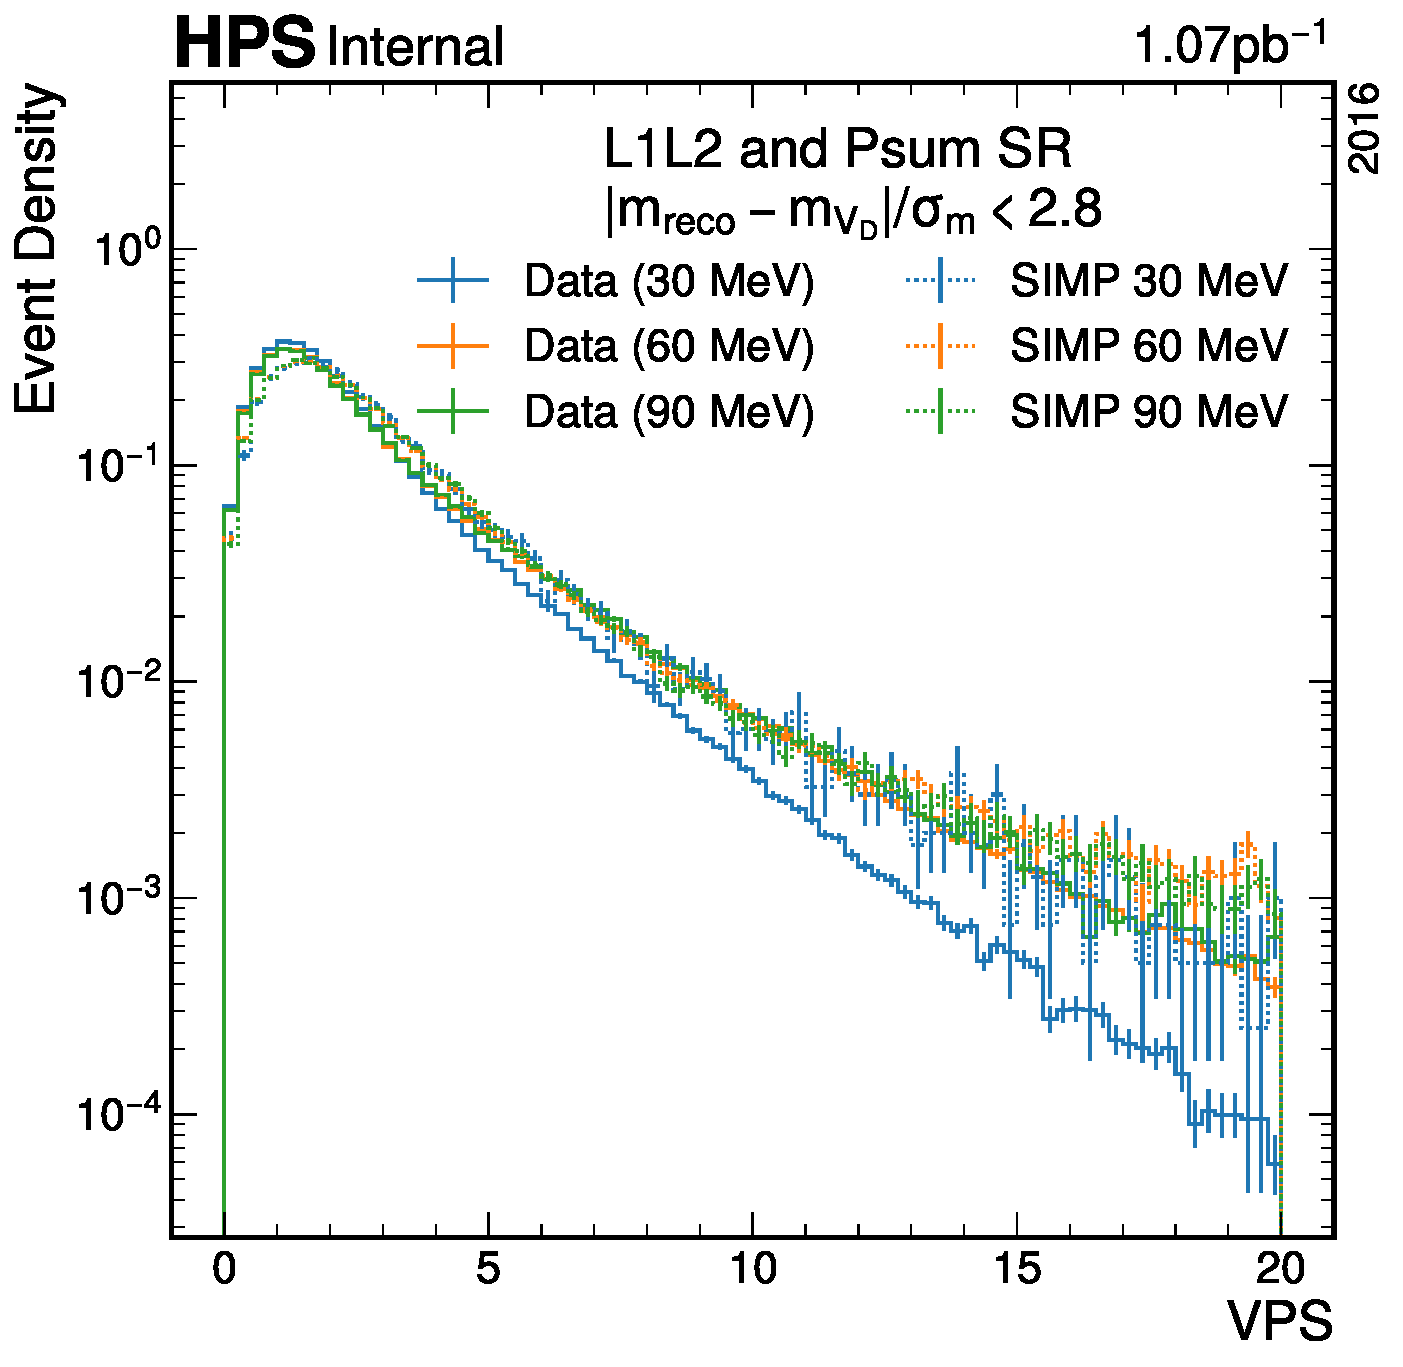
\includegraphics[width=\textwidth]{figures/hps/analysis/vtx_proj_sig-distribution.pdf}
    \caption{\ac{vps}}
    \label{fig:data-signal-comp:vps}
  \end{subfigure}
  ~
  \begin{subfigure}{0.30\textwidth}
    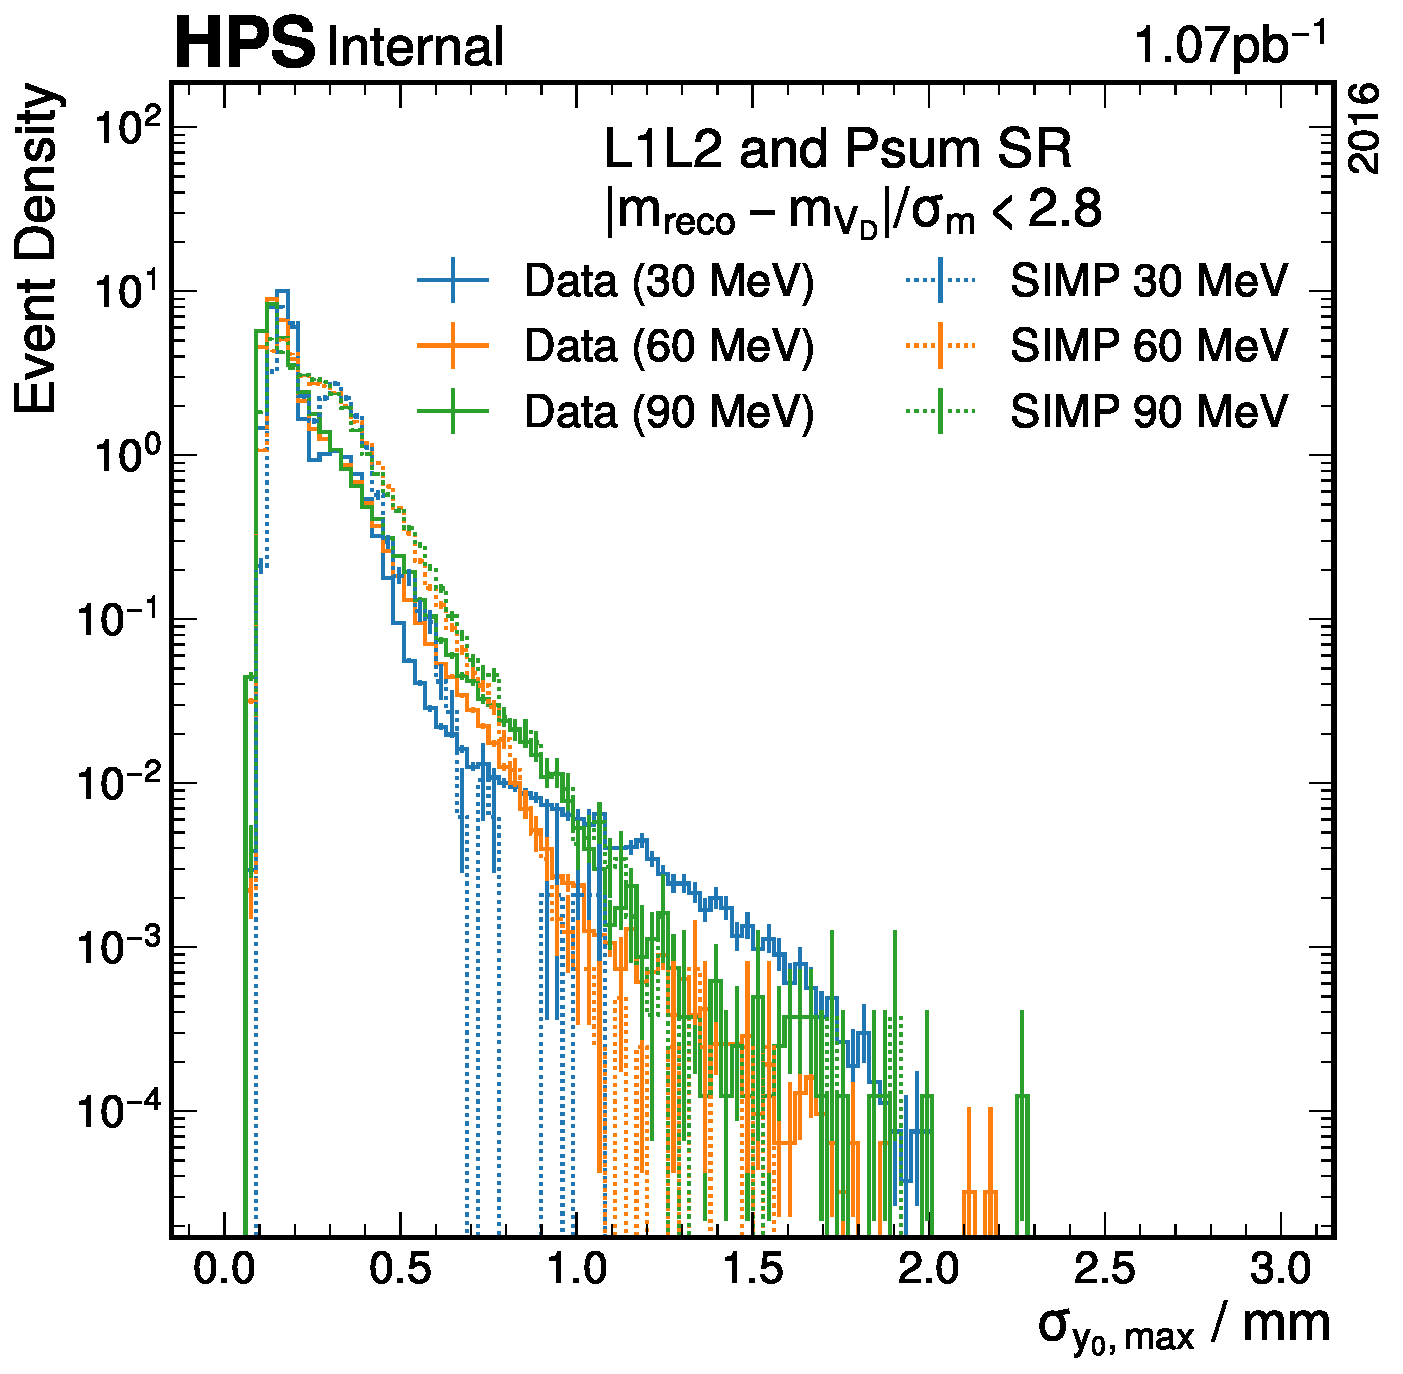
\includegraphics[width=\textwidth]{figures/hps/analysis/max_y0_err-distribution.pdf}
    \caption{\maxyzeroerr}
    \label{fig:data-signal-comp:max-y0-err}
  \end{subfigure}
  ~
  \begin{subfigure}{0.30\textwidth}
    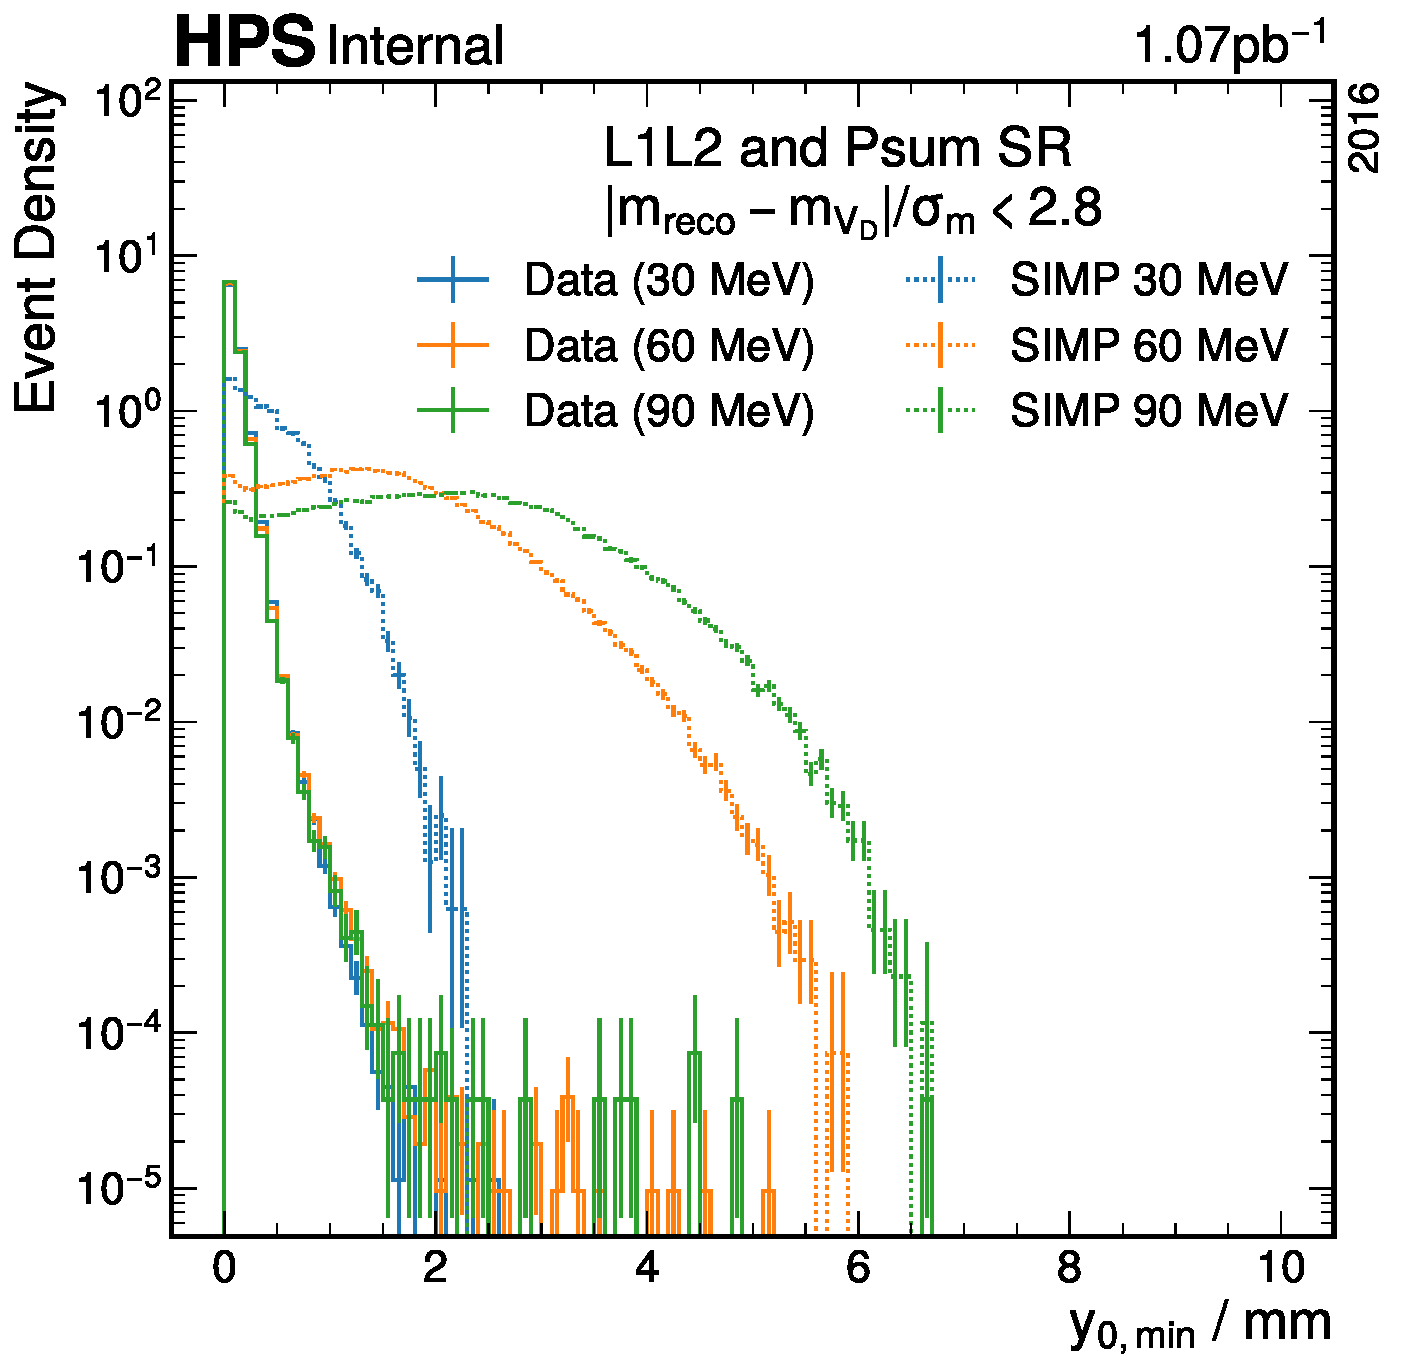
\includegraphics[width=\textwidth]{figures/hps/analysis/min_y0-distribution.pdf}
    \caption{\minyzero}
    \label{fig:data-signal-comp:min-y0}
  \end{subfigure}
  \caption{%
    Distributions of cut variables for a few example mass points.
    The vertices are required to be L1L2, have their momentum sum be within
    the signal region, and their invariant mass within the specified mass window.
  }
  \label{fig:data-signal-comp}
\end{figure}

Vertex $z$ is left for late-stage statistical analysis of the results
and -- being highly correlated with \minyzero -- is redundant with this variable.


\part{Conclusion} \label{part:conclusion}
\chapter{Conclusion}
\label{chapter:conclusion}

Both \ac{ldmx} and \ac{hps} are important and required experiments in our search
for the particle nature of \ac{dm}.
While neither has progressed far enough to exclude new parameter space
(or potentially discover \ac{dm} that was previously out of reach),
both experiments take novel approaches towards this search.
These approaches are required because the traditional tactics have not
yielded discovery and are unable to reach into these specific regions
of parameter space.

The \ac{ldmx} \ac{eat} analysis presented here is novel for \ac{ldmx}
not only due to the missing-energy search style, but also because we
took care to estimate the magnitude of potential systematic errors,
form a quantitative non-zero background prediction with its own
statistical uncertainty, and performed the statistical analysis
over several bins.
Previous \ac{ldmx} analyses focusing on zero-background searches,
while important and interesting in their own right, do not have the
flexibility necessary to be an analysis used with data collected
form a newly built apparatus.
The \ac{eat} analysis channel is such an analysis and it is well
prepared to be the first analysis of \ac{ldmx} data making new
physics conclusions about our universe.

The \ac{hps} \ac{simp} L1L2 analysis extended the \ac{simp} search
to a previously-unexplored reconstruction category, enabling us to
use a larger fraction of the data already collected by \ac{hps}.
This \ac{simp} search, while not excluding new phase space with the
current data set, shows promise.
We have been able to show that a displaced-vertex search with
the possibility of missing energy is possible.
Extending such a search to unexplored phase space, an area where no
other experiments have access, is simply awaiting the necessary
reconstruction studies in order to analyze later and larger data
sets already collected by the detector.

As newer and smaller experiments compared to other \ac{hep} experiments,
different excitements and difficulties arise.
While participating in the full breadth of a particle physics experiment
has taught me a lot and given me opportunity to carve my own path of learning,
the lack of larger support structures has revealed some specifically intricate
problems that \ac{ldmx} and \ac{hps} share.

\section{Simulation Validity}
The design and initial studies of any experiment requires some simulation
of the measurements it could perform.
After the experiment has been constructed and collects data, the simulation
is still incredibly useful for studying how \emph{known} processes present
themselves within the observations.
The collected data \emph{could} have a previously-unknown and rare process
within it, so we must be careful to avoid biasing our analysis in such a
way that would ruin the validity of our results.
A reasonable strategy is simply to avoid studying all of the data at once
and instead design and optimize the analysis on a particular subset of the
data.
This process is called ``blinding'' and was used in \cref{part:hps};
however, this also naturally means the analysis can easily be optimized
only for the special events within the subset and the events outside of
this subset are unaccounted for.

A valid simulation, one which correctly predicts the scale and shape
of the observable distributions, is a valuable tool that could partially
or completely replace this blinding procedure.
In this case, the simulated observations could be used to help design
and optimize the analysis; avoiding bias while also allowing the analysis
to explore the full breadth of potential events that could be seen.

While the ``valid simulation'' I describe here is not necessarily possible,
we can move forward towards it in order to make future analyses better.
One of the first studies that will be done with new \ac{ldmx} data will
be comparing how our simulated events compare to the events actually being
collected by the real detector.
Returning to these comparisons for \ac{hps} and its subsequent, larger
sets of data is being done and will be beneficial for those analyses as well
especially given the separation between data and simulation already being
observed within the pre-selection (for example, in \cref{fig:vertex-pre-selection}).

\section{Tracking Reconstruction}
Most of my work on tracking and the alignment of a tracking detector
was done within the context of \ac{hps}.
This particular tracking detector is somewhat of a ``trial by fire'' due
to its delicate, two-sided nature required by the specific physics for
which we are searching.
Nevertheless, this experience has given me a solid introduction to charged
particle tracking.

As discussed in \cref{chapter:hps:alignment}, charged particle tracking is
very complicated and it almost certainly requires familiarity with the
equally-complicated process of alignment.
Going forward, both \ac{ldmx} and \ac{hps} require robust and solid tracking
software in order to make the interpretations of such intricate algorithms simpler.
Without the backing of a larger collaboration to more completely test
and validate this complicated software, using a shared tracking framework
like ACTS\cite{acts} is necessary, a strategy starting to be employed in both
experiments.

\section{Reflection}
This dissertation work has shown me the full breadth of a particle physics experiment.
From initial design and simulation, to extensions and validations of said simulation,
to intricate considerations of potential systematic errors in the experiment,
to optimization of selections using various figures of merit,
to intentional analysis blinding to avoid statistical bias when developing an analysis,
to final unblinding after proposals and evaluations,
to post-mortem analysis of the leftover bits of data.

While I have not documented all of these steps within this document,
they all brought with them lessons for which I am grateful.

%%%%%%%%%%%%%%%%%%%%%%%%%%%%%%%%%%%%%%%%%%%%%%%%%%%%%%%%%%%%%%%%%%%%%%%%%%%%%%%%

%%%%%%%%%%%%%%%%%%%%%%%%%%%%%%%%%%%%%%%%%%%%%%%%%%%%%%%%%%%%%%%%%%%%%%%%%%%%%%%%
% Bibliography
%%%%%%%%%%%%%%%%%%%%%%%%%%%%%%%%%%%%%%%%%%%%%%%%%%%%%%%%%%%%%%%%%%%%%%%%%%%%%%%%
\bibliography{thesis}
%%%%%%%%%%%%%%%%%%%%%%%%%%%%%%%%%%%%%%%%%%%%%%%%%%%%%%%%%%%%%%%%%%%%%%%%%%%%%%%%

%%%%%%%%%%%%%%%%%%%%%%%%%%%%%%%%%%%%%%%%%%%%%%%%%%%%%%%%%%%%%%%%%%%%%%%%%%%%%%%%
% Appendices
%%%%%%%%%%%%%%%%%%%%%%%%%%%%%%%%%%%%%%%%%%%%%%%%%%%%%%%%%%%%%%%%%%%%%%%%%%%%%%%%
\part{Appendices}
\appendix
%%%%%%%%%%%%%%%%%%%%%%%%%%%%%%%%%%%%%%%%%%%%%%%%%%%%%%%%%%%%%%%%%%%%%%%%%%%%%%%%
\todos

%%%%%%%%%%%%%%%%%%%%%%%%%%%%%%%%%%%%%%%%%%%%%%%%%%%%%%%%%%%%%%%%%%%%%%%%%%%%%%%%
% End the Document
%%%%%%%%%%%%%%%%%%%%%%%%%%%%%%%%%%%%%%%%%%%%%%%%%%%%%%%%%%%%%%%%%%%%%%%%%%%%%%%%
\end{document}
%%%%%%%%%%%%%%%%%%%%%%%%%%%%%%%%%%%%%%%%%%%%%%%%%%%%%%%%%%%%%%%%%%%%%%%%%%%%%%%%
